%\section{Systematics Uncertainties on the Background Prediction}
%\label{sec:systematics}

In this Section we discuss the systematic uncertainty on the BG
prediction.  This prediction is assembled from the event
counts in the peak region of the transverse mass distribution as
well as Monte Carlo 
with a number of correction factors, as described previously.
The
final uncertainty on the prediction is built up from the uncertainties in these
individual 
components. 
The calculation is done for each signal
region,
for electrons and muons separately.

The choice to normalize to the peak region of $M_T$ has the
advantage that some uncertainties, e.g., luminosity, cancel.
It does however introduce complications because it couples
some of the uncertainties in non-trivial ways.  For example, 
the primary effect of an uncertainty on the rare MC cross-section
is to introduce an uncertainty in the rare MC background estimate
which comes entirely from MC.   But this uncertainty also affects,
for example,
the $t\bar{t} \to$ dilepton BG estimate because it changes the 
$t\bar{t}$ normalization to the peak region (because some of the 
events in the peak region are from rare processes).  These effects
are carefully accounted for. The contribution to the overall
uncertainty from each background source is tabulated in
Section~\ref{sec:bgunc-bottomline}.
Here we discuss the uncertainties one-by-one and comment 
on their impact on the overall result, at least to first order.
Second order effects, such as the one described, are also included.

\subsection{Statistical uncertainties on the event counts in the $M_T$
peak regions}
These vary between 2\% and 20\%, depending on the signal region
(different
signal regions have different \met\ requirements, thus they also have
different $M_T$ regions used as control).
Since 
the major backgrounds, eg, $t\bar{t}$ are normalized to the peak regions, this 
fractional uncertainty is pretty much carried through all the way to
the end.  There is also an uncertainty from the finite MC event counts
in the $M_T$ peak regions.  This is also included, but it is smaller.

Normalizing to the $M_T$ peak has the distinct advantages that 
uncertainties on luminosity, cross-sections, trigger efficiency,
lepton ID, cancel out.
For the low statistics regions with high \met\ requirements, the
price to pay in terms of event count is that statistical uncertainties start
to become significant.  In the future we may consider a different
normalization startegy in the low statistics regions.

\subsection{Uncertainty from the choice of $M_T$ peak region}

This choice affects the scale factors of Table~\ref{tab:mtpeaksf}.  
If the $M_T$ peak region is not well modelled, this would introduce an
uncertainty.

We have tested this possibility by recalculating the post-veto scale factors for a different
choice
of $M_T$ peak region ($40 < M_T < 100$ GeV instead of the default
$50 < M_T < 80$ GeV).  This is shown in Table~\ref{tab:mtpeaksf2}.  
The two results for the scale factors are very compatible. 
We do not take any systematic uncertainty for this possible effect.

\begin{table}[!h]
\begin{center}
{\footnotesize
\begin{tabular}{l||c|c|c|c|c|c|c}
\hline
Sample              & SRA & SRB & SRC & SRD & SRE & SRF & SRG\\
\hline
\hline
\multicolumn{8}{c}{$50 \leq \mt \leq 80$} \\
\hline
$\mu$ pre-veto \mt-SF      & $1.02 \pm 0.02$ & $0.95 \pm 0.03$ & $0.90 \pm 0.05$ & $0.98 \pm 0.08$ & $0.97 \pm 0.13$ & $0.85 \pm 0.18$ & $0.92 \pm 0.31$ \\
$\mu$ post-veto \mt-SF     & $1.00 \pm 0.02$ & $0.95 \pm 0.03$ & $0.91 \pm 0.05$ & $1.00 \pm 0.09$ & $0.99 \pm 0.13$ & $0.85 \pm 0.18$ & $0.96 \pm 0.31$ \\
\hline
$\mu$ veto \mt-SF          & $0.98 \pm 0.01$ & $0.99 \pm 0.01$ & $1.01 \pm 0.02$ & $1.02 \pm 0.04$ & $1.02 \pm 0.06$ & $1.00 \pm 0.09$ & $1.04 \pm 0.11$ \\
\hline
\hline
e pre-veto \mt-SF          & $0.95 \pm 0.02$ & $0.95 \pm 0.03$ & $0.94 \pm 0.06$ & $0.85 \pm 0.09$ & $0.84 \pm 0.13$ & $1.05 \pm 0.23$ & $1.04 \pm 0.33$ \\
e post-veto \mt-SF         & $0.92 \pm 0.02$ & $0.91 \pm 0.03$ & $0.91 \pm 0.06$ & $0.74 \pm 0.08$ & $0.75 \pm 0.13$ & $0.91 \pm 0.22$ & $1.01 \pm 0.33$ \\
\hline
e veto \mt-SF      & $0.97 \pm 0.01$ & $0.96 \pm 0.02$ & $0.97 \pm 0.03$ & $0.87 \pm 0.05$ & $0.89 \pm 0.08$ & $0.86 \pm 0.11$ & $0.97 \pm 0.14$ \\
\hline
\hline
\multicolumn{8}{c}{$40 \leq \mt \leq 100$} \\
\hline
$\mu$ pre-veto \mt-SF      & $1.02 \pm 0.01$ & $0.97 \pm 0.02$ & $0.91 \pm 0.05$ & $0.95 \pm 0.06$ & $0.97 \pm 0.10$ & $0.80 \pm 0.14$ & $0.74 \pm 0.22$ \\
$\mu$ post-veto \mt-SF     & $1.00 \pm 0.01$ & $0.96 \pm 0.02$ & $0.90 \pm 0.04$ & $0.98 \pm 0.07$ & $1.00 \pm 0.11$ & $0.80 \pm 0.15$ & $0.81 \pm 0.24$ \\
\hline
$\mu$ veto \mt-SF          & $0.98 \pm 0.01$ & $0.99 \pm 0.01$ & $0.99 \pm 0.02$ & $1.03 \pm 0.03$ & $1.03 \pm 0.05$ & $1.01 \pm 0.08$ & $1.09 \pm 0.09$ \\
\hline
\hline
e pre-veto \mt-SF          & $0.97 \pm 0.01$ & $0.93 \pm 0.02$ & $0.94 \pm 0.04$ & $0.81 \pm 0.06$ & $0.86 \pm 0.10$ & $0.95 \pm 0.17$ & $1.06 \pm 0.26$ \\
e post-veto \mt-SF         & $0.94 \pm 0.01$ & $0.91 \pm 0.02$ & $0.91 \pm 0.04$ & $0.71 \pm 0.06$ & $0.82 \pm 0.10$ & $0.93 \pm 0.17$ & $1.09 \pm 0.27$ \\
\hline
e veto \mt-SF      & $0.97 \pm 0.01$ & $0.98 \pm 0.01$ & $0.97 \pm 0.02$ & $0.88 \pm 0.04$ & $0.95 \pm 0.06$ & $0.98 \pm 0.08$ & $1.03 \pm 0.09$ \\
\hline
\end{tabular}}
\caption{ \mt\ peak Data/MC scale factors. The pre-veto SFs are applied to the
  \ttdl\ sample, while the post-veto SFs are applied to the single
  lepton samples. The veto SF is shown for comparison across channels.
  The raw MC is used for backgrounds from rare processes.
  The uncertainties are statistical only.
\label{tab:mtpeaksf2}}
\end{center}
\end{table}


\subsection{Uncertainty on the \wjets\ cross-section and the rare MC cross-sections}
These are taken as 50\%, uncorrelated.  
The primary effect is to introduce a 50\%
uncertainty
on the $W +$ jets and rare BG 
background predictions, respectively.  However they also
have an effect on the other BGs via the $M_T$ peak normalization
in a way that tends to reduce the uncertainty.  This is easy
to understand: if the $W$ cross-section is increased by 50\%, then
the $W$ background goes up.  But the number of $M_T$ peak events 
attributed to $t\bar{t}$ goes down, and since the $t\bar{t}$ BG is
scaled to the number of $t\bar{t}$ events in the peak, the $t\bar{t}$ 
BG goes down.  

\subsection{Tail-to-peak ratios for lepton +
  jets top and W events}
The tail-to-peak ratios $R_{top}$ and $R_{wjet}$ are described in Section~\ref{sec:ttp}.
The data/MC scale factors are studied in CR1 and CR2 (Sections~\ref{sec:cr1} and~\ref{sec:cr2}).
Only the scale factor for \wjets, $SFR_{wjet}$, is used, and its
uncertainty is given in Table~\ref{tab:cr1yields}. 
This uncertainty affects both $R_{wjet}$ and $R_{top}$.
The additional systematic uncertainty on $R_{top}$ from the variation between optimistic and pessimistic scenarios is given in Section~\ref{sec:ttp}. 


\subsection{Uncertainty on extra jet radiation for dilepton
  background}
As discussed in Section~\ref{sec:jetmultiplicity}, the 
jet distribution in
$t\bar{t} \to$
dilepton MC is rescaled by the factors $K_3$ and $K_4$ to make 
it agree with the data.  The 3\% uncertainties on $K_3$ and $K_4$
comes from data/MC statistics.  This  
results directly in a 3\% uncertainty on the dilepton background, which is by far 
the most important one.

\subsection{Uncertainty from MC statistics}
This affects mostly the \ttll\ background estimate, which is taken
from
Monte Carlo with appropriate correction factors.  This uncertainty
is negligible in the low \met\ signal regions, and grows to about
15\% in SRG.


\subsection{Uncertainty on the \ttll\ Background}
\label{sec:ttdilbkgunc}
The \ttbar\ background prediction is obtained from MC, with corrections
derived from control samples in data. The uncertainty associated with
the \ttbar\ background is derived from the level of closure of the
background prediction in CR4 (Table~\ref{tab:cr4yields}) and 
CR5 (Table~\ref{tab:cr5yields}). The results from these control region
checks are shown in Figure~\ref{fig:ttdlunc}. The uncertainties assigned
to the \ttdl\ background prediction based on these tests are 
5\% (SRA), 10\% (SRB), 15\% (SRC), 25\% (SRD), 40\% (SRE-G).

\begin{figure}[hbt]
  \begin{center}
        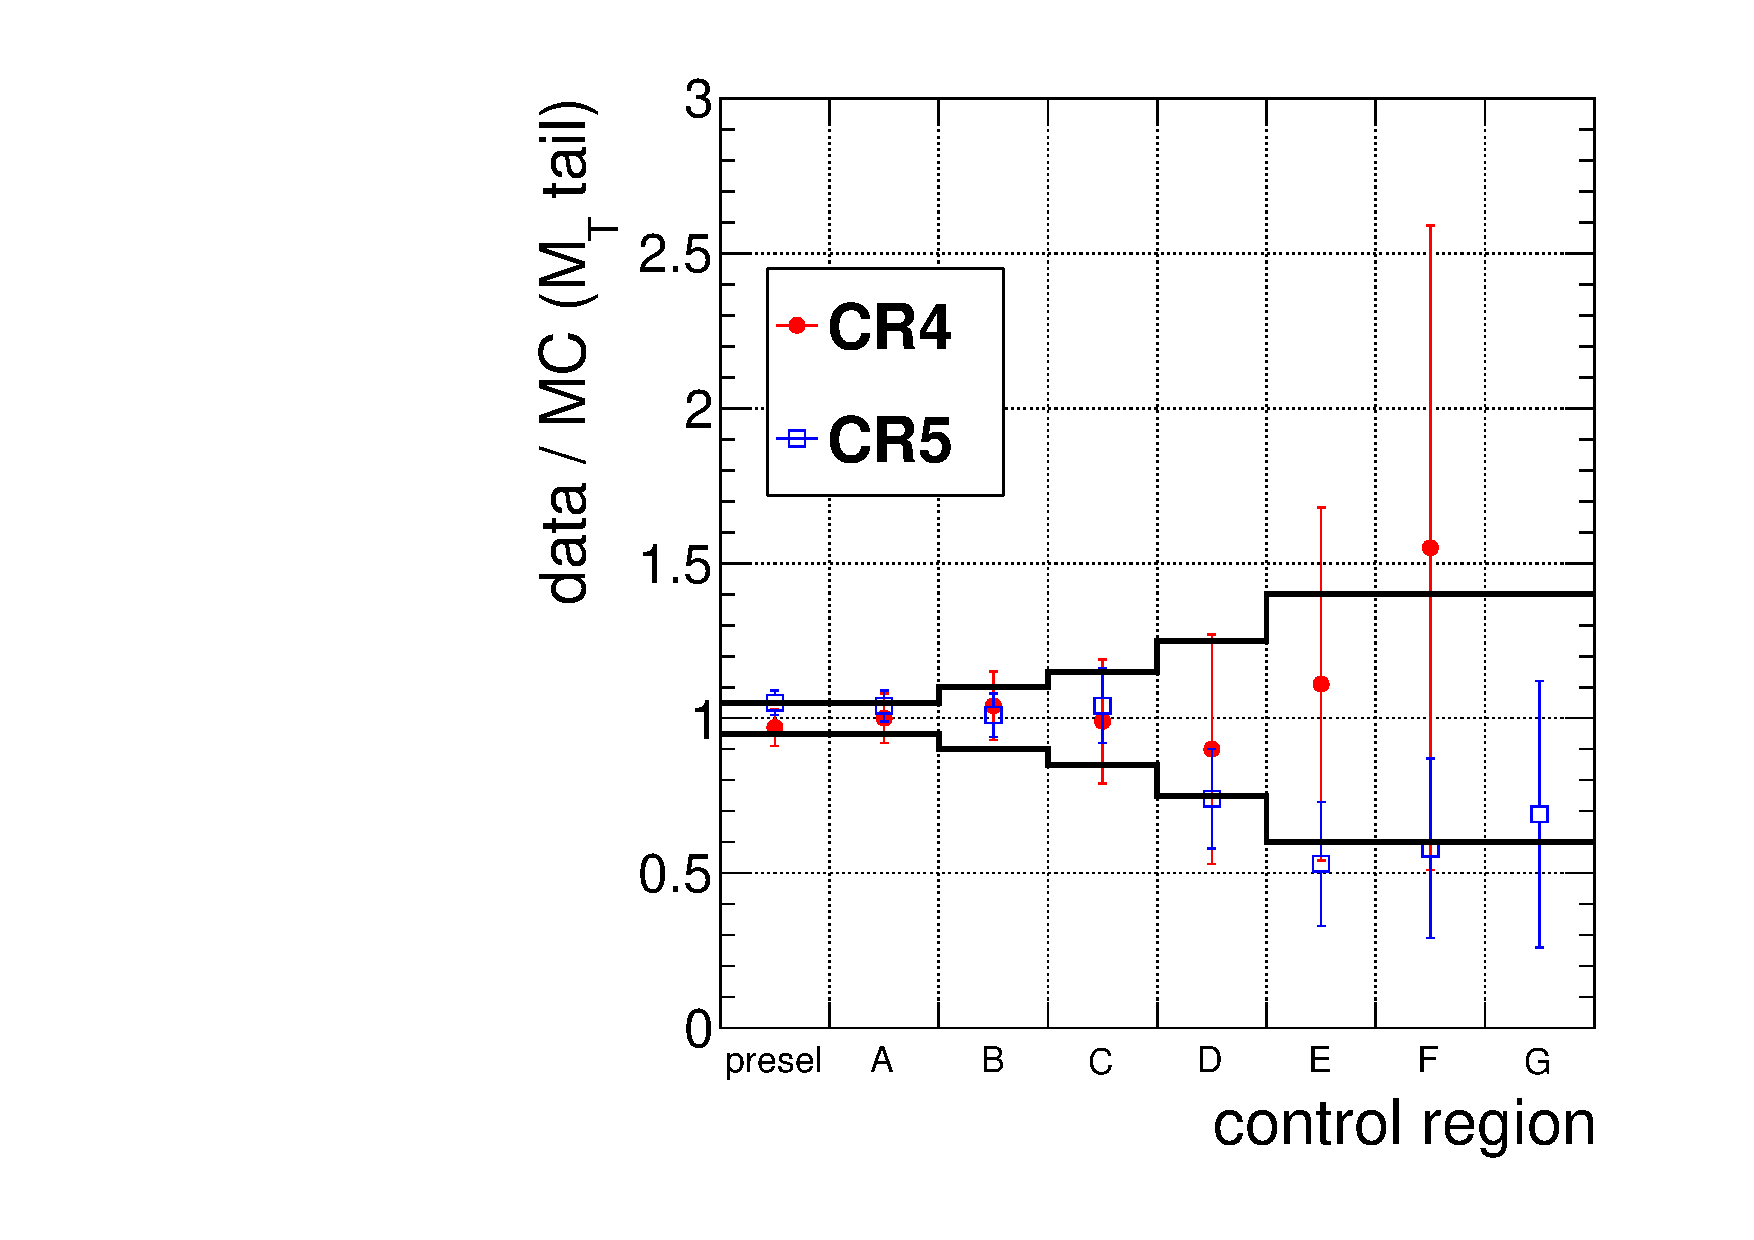
\includegraphics[width=0.6\linewidth]{plots/ttdilepton_uncertainty.pdf}
        \caption{
          \label{fig:ttdlunc}%\protect 
          Results of the comparison of yields in the \mt\ tail comparing the MC prediction (after
          applying SFs) to data for CR4 and CR5 for all the signal
          region requirements considered (A-G). The bands indicate the
          systematic uncertainties assigned based on these tests,
          ranging from $5\%$ for SRA to $40\%$ for SRE-G.}
      \end{center}
\end{figure}

\clearpage
\subsubsection{Check of the impact of Signal Contamination}

We examine the contribution of possible signal events in the \ttll\
control regions (CR4 and CR5). It should be emphasized that these 
regions are not used to apply data/MC SFs. They are used to quantify 
the level of data/MC agreement and assign a corresponding uncertainty.

To illustrate how much signal is expected to populate these control
regions, we examine signal points near the edge of the analysis'
sensitivity (m(stop) = 450 m($\chi^0$) = 0 for T2tt, m(stop) = 450 
m($\chi^0$) = 0 for T2bw with x=0.75 and m(stop) = 350 
m($\chi^0$) = 0 for T2bw with x=0.5). 
Table~\ref{tab:signalcontamination} compares the expected signal
yields and the raw total MC background prediction in the control
regions with the \met\ and \mt\ requirements corresponding to SRB, SRC
and SRD (these are the signal regions that dominate the
sensitivity). The signal contamination is smaller than the uncertainty
on the dilepton background and smaller than the signal/background in
the signal regions, with the exception of the T2bw scenario with x=0.5.
However, based on the fact that the CR4 and CR5 are not used to extract
data/MC SFs and that CR4 shows a slight deficit of data compared to
the MC prediction, indicating that we do not observe evidence of
signal contamination, we do not assign an additional uncertainty.

\begin{table}[!h]
\begin{center}
{\small
\begin{tabular}{l l||c|c|c}
\hline
\multicolumn{2}{c||}{Sample}              & CR B & CR C & CR D \\
\hline
\hline
\multirow{4}{*}{CR4} & Raw MC            & $168.2 \pm 4.5$& $51.5 \pm 2.5$& $19.6 \pm 1.5$ \\
%\hline
& T2tt m(stop) = 450 m($\chi^0$) = 0  & $2.6 \pm 0.3$ $(2\%)$ & $2.0 \pm 0.2$ $(4\%)$ & $1.4 \pm 0.2$ $(7\%)$ \\
& T2bw x=0.75 m(stop) = 450 m($\chi^0$) = 0 & $10.5 \pm 0.4$ $(6\%)$ &$6.1 \pm 0.3$ $(12\%)$ & $3.1 \pm 0.2$ $(16\%)$ \\
& T2bw x=0.5  m(stop) = 350 m($\chi^0$) = 0 	& $32.1 \pm 1.5$ $(19\%)$ & $14.7 \pm 1.0$ $(29\%)$ & $5.5 \pm 0.6$ $(28\%)$ \\
\hline
\hline
\multirow{4}{*}{CR5} & Raw MC            & $306.5 \pm 6.2$& $101.8 \pm 3.6$& $38.0 \pm 2.2$ \\
%\hline
& T2tt m(stop) = 450 m($\chi^0$) = 0  & $10.6 \pm 0.6$ $(3\%)$ & $7.8 \pm 0.5$ $(8\%)$ & $5.4 \pm 0.4$ $(14\%)$ \\
& T2bw x=0.75 m(stop) = 450 m($\chi^0$) = 0 & $17.3 \pm 0.5$ $(6\%)$ &$11.3 \pm 0.4$ $(11\%)$ & $6.2 \pm 0.3$ $(16\%)$\\
& T2bw x=0.5  m(stop) = 350 m($\chi^0$) = 0 	& $33.0 \pm 1.5$ $(11\%)$& $14.4 \pm 1.0$ $(14\%)$& $5.7 \pm 0.6$ $(15\%)$ \\
\hline
\hline
\hline
\multirow{4}{*}{SIGNAL} & Raw MC 		 & $486.3 \pm 7.8$& $164.3 \pm 4.5$& $61.5 \pm 2.8$ \\
& T2tt m(stop) = 450 m($\chi^0$) = 0 	& $65.3 \pm 1.4$ $(13\%)$& $48.8 \pm 1.2$ $(30\%)$& $32.9 \pm 1.0$ $(53\%)$ \\
& T2bw x=0.75 m(stop) = 450 m($\chi^0$) = 0 	& $69.3 \pm 1.0$ $(14\%)$& $47.3 \pm 0.8$ $(29\%)$& $27.3 \pm 0.6$ $(44\%)$ \\
& T2bw x=0.5  m(stop) = 350 m($\chi^0$) = 0 	& $105.5 \pm 2.8$ $(22\%)$& $44.6 \pm 1.8$ $(27\%)$& $15.9 \pm 1.1$ $(26\%)$ \\
\hline
\end{tabular}}
\caption{ Yields in \mt\ tail comparing the raw SM MC prediction to the
  yields for a few signal points on the edge of our sensitivity in the \ttll\
  control regions CR4, CR5 and in the corresponding signal region.
  The numbers in parenthesis are the expected signal yield divided by
  the total background. The uncertainties are statistical only.
\label{tab:signalcontamination}}
\end{center}
\end{table}

%CR5 DUMP
%Total 		 & $880.3 \pm 10.4$& $560.0 \pm 8.3$& $306.5 \pm 6.2$& $101.8 \pm 3.6$& $38.0 \pm 2.2$& $16.4 \pm 1.4$& $8.2 \pm 1.0$& $4.6 \pm 0.8$ \\
%\hline
%\hline
%Data 		 & $941$& $559$& $287$& $95$& $26$& $8$& $5$& $3$ \\
%\hline
%T2tt m(stop) = 250 m($\chi^0$) = 0 	& $84.3 \pm 9.2$& $61.9 \pm 7.9$& $35.7 \pm 6.0$& $5.9 \pm 2.4$& $1.0 \pm 1.0$& $1.0 \pm 1.0$& $0.0 \pm 0.0$& $0.0 \pm 0.0$ \\
%\hline
%T2tt m(stop) = 300 m($\chi^0$) = 50 	& $61.4 \pm 4.7$& $53.6 \pm 4.4$& $42.0 \pm 3.9$& $14.3 \pm 2.3$& $7.2 \pm 1.6$& $1.8 \pm 0.8$& $0.7 \pm 0.5$& $0.0 \pm 0.0$ \\
%\hline
%T2tt m(stop) = 300 m($\chi^0$) = 100 	& $33.3 \pm 3.5$& $28.6 \pm 3.2$& $19.2 \pm 2.6$& $6.1 \pm 1.5$& $1.8 \pm 0.8$& $0.4 \pm 0.4$& $0.4 \pm 0.4$& $0.4 \pm 0.4$ \\
%\hline
%T2tt m(stop) = 350 m($\chi^0$) = 0 	& $33.4 \pm 2.2$& $29.8 \pm 2.1$& $27.3 \pm 2.0$& $15.3 \pm 1.5$& $5.6 \pm 0.9$& $1.9 \pm 0.5$& $0.3 \pm 0.2$& $0.0 \pm 0.0$ \\
%\hline
%T2tt m(stop) = 450 m($\chi^0$) = 0 	& $12.0 \pm 0.6$& $11.3 \pm 0.6$& $10.6 \pm 0.6$& $7.8 \pm 0.5$& $5.4 \pm 0.4$& $3.1 \pm 0.3$& $1.8 \pm 0.2$& $0.6 \pm 0.1$ \\
%\hline
%T2bw m(stop) = 350 x=0.5 m($\chi^0$) = 0 	& $48.5 \pm 1.9$& $40.2 \pm 1.7$& $33.0 \pm 1.5$& $14.4 \pm 1.0$& $5.7 \pm 0.6$& $2.7 \pm 0.4$& $1.3 \pm 0.3$& $0.5 \pm 0.2$ \\
%\hline
%T2bw m(stop) = 450 x=0.75 m($\chi^0$) = 0 	& $22.3 \pm 0.6$& $20.2 \pm 0.6$& $17.3 \pm 0.5$& $11.3 \pm 0.4$& $6.2 \pm 0.3$& $3.1 \pm 0.2$& $1.3 \pm 0.1$& $0.7 \pm 0.1$ \\
%\hline

%CR4 DUMP
%\hline
%Total 		 & $510.1 \pm 8.0$& $324.2 \pm 6.3$& $168.2 \pm 4.5$& $51.5 \pm 2.5$& $19.6 \pm 1.5$& $7.8 \pm 1.0$& $2.6 \pm 0.6$& $1.1 \pm 0.3$ \\
%\hline
%\hline
%Data 		 & $462$& $289$& $169$& $45$& $10$& $7$& $5$& $3$ \\
%\hline
%T2tt m(stop) = 250 m($\chi^0$) = 0 	& $37.7 \pm 6.1$& $30.9 \pm 5.5$& $18.0 \pm 4.2$& $6.0 \pm 2.5$& $2.0 \pm 1.4$& $0.0 \pm 0.0$& $0.0 \pm 0.0$& $0.0 \pm 0.0$ \\
%\hline
%T2tt m(stop) = 300 m($\chi^0$) = 50 	& $16.6 \pm 2.4$& $14.4 \pm 2.3$& $11.3 \pm 2.0$& $5.6 \pm 1.4$& $3.2 \pm 1.1$& $1.8 \pm 0.8$& $0.0 \pm 0.0$& $0.0 \pm 0.0$ \\
%\hline
%T2tt m(stop) = 300 m($\chi^0$) = 100 	& $9.6 \pm 1.8$& $6.4 \pm 1.5$& $4.6 \pm 1.3$& $0.7 \pm 0.5$& $0.4 \pm 0.4$& $0.0 \pm 0.0$& $0.0 \pm 0.0$& $0.0 \pm 0.0$ \\
%\hline
%T2tt m(stop) = 350 m($\chi^0$) = 0 	& $8.2 \pm 1.1$& $7.6 \pm 1.0$& $5.7 \pm 0.9$& $3.4 \pm 0.7$& $1.9 \pm 0.5$& $0.6 \pm 0.3$& $0.3 \pm 0.2$& $0.1 \pm 0.1$ \\
%\hline
%T2tt m(stop) = 450 m($\chi^0$) = 0 	& $3.1 \pm 0.3$& $2.9 \pm 0.3$& $2.6 \pm 0.3$& $2.0 \pm 0.2$& $1.4 \pm 0.2$& $1.0 \pm 0.2$& $0.4 \pm 0.1$& $0.2 \pm 0.1$ \\
%\hline
%T2bw m(stop) = 350 x=0.5 m($\chi^0$) = 0 	& $52.6 \pm 1.9$& $42.6 \pm 1.7$& $32.1 \pm 1.5$& $14.7 \pm 1.0$& $5.5 \pm 0.6$& $1.9 \pm 0.4$& $0.6 \pm 0.2$& $0.3 \pm 0.1$ \\
%\hline
%T2bw m(stop) = 450 x=0.75 m($\chi^0$) = 0 	& $16.9 \pm 0.5$& $14.9 \pm 0.5$& $10.5 \pm 0.4$& $6.1 \pm 0.3$& $3.1 \pm 0.2$& $1.5 \pm 0.1$& $0.6 \pm 0.1$& $0.3 \pm 0.1$ \\
%\hline


\subsubsection{Check of the uncertainty on the \ttll\ Background}

We check that the systematic uncertainty assigned to the \ttll\ background prediction
covers the uncertainty associated with
the theoretical modeling of the \ttbar\ production and decay
by comparing the background predictions obtained using 
alternative MC samples. It should be noted that the full analysis is
performed with the alternative samples under consideration, 
including the derivation of the various data-to-MC scale factors. 
The variations considered are

\begin{itemize}
\item Top mass: The alternative values for the top mass differ
  from the central value by $6~\GeV$: $m_{\mathrm{top}} = 178.5~\GeV$ and $m_{\mathrm{top}}
  = 166.5~\GeV$.
\item Jet-parton matching scale: This corresponds to variations in the
  scale at which the Matrix Element partons from Madgraph are matched
  to Parton Shower partons from Pythia. The nominal value is
  $x_q>20~\GeV$. The alternative values used are $x_q>10~\GeV$ and
  $x_q>40~\GeV$.
\item Renormalization and factorization scale: The alternative samples
  correspond to variations in the scale $\times 2$ and $\times 0.5$. The nominal
  value for the scale used is $Q^2 = m_{\mathrm{top}}^2 +
  \sum_{\mathrm{jets}} \pt^2$.
\item Alternative generators: Samples produced with different
  generators, Powheg (our default) and Madgraph.
\item Modeling of taus: The alternative sample does not include
  Tauola and is otherwise identical to the Powheg sample.
  This effect was studied earlier using 7~TeV samples and found to be negligible.
\item The PDF uncertainty is estimated following the PDF4LHC
  recommendations. The events are reweighted using alternative
  PDF sets for CT10 and MSTW2008 and the uncertainties for each are derived using the
  alternative eigenvector variations and the ``master equation''.
  The NNPDF2.1 set with 100 replicas is also used. The central value is
  determined from the mean and the uncertainty is derived from the
  $1\sigma$ range. The overall uncertainty is derived from the envelope of the
  alternative predictions and their uncertainties.
  This effect was studied earlier using 7~TeV samples and found to be negligible.
  \end{itemize}

\begin{figure}[hbt]
  \begin{center}
	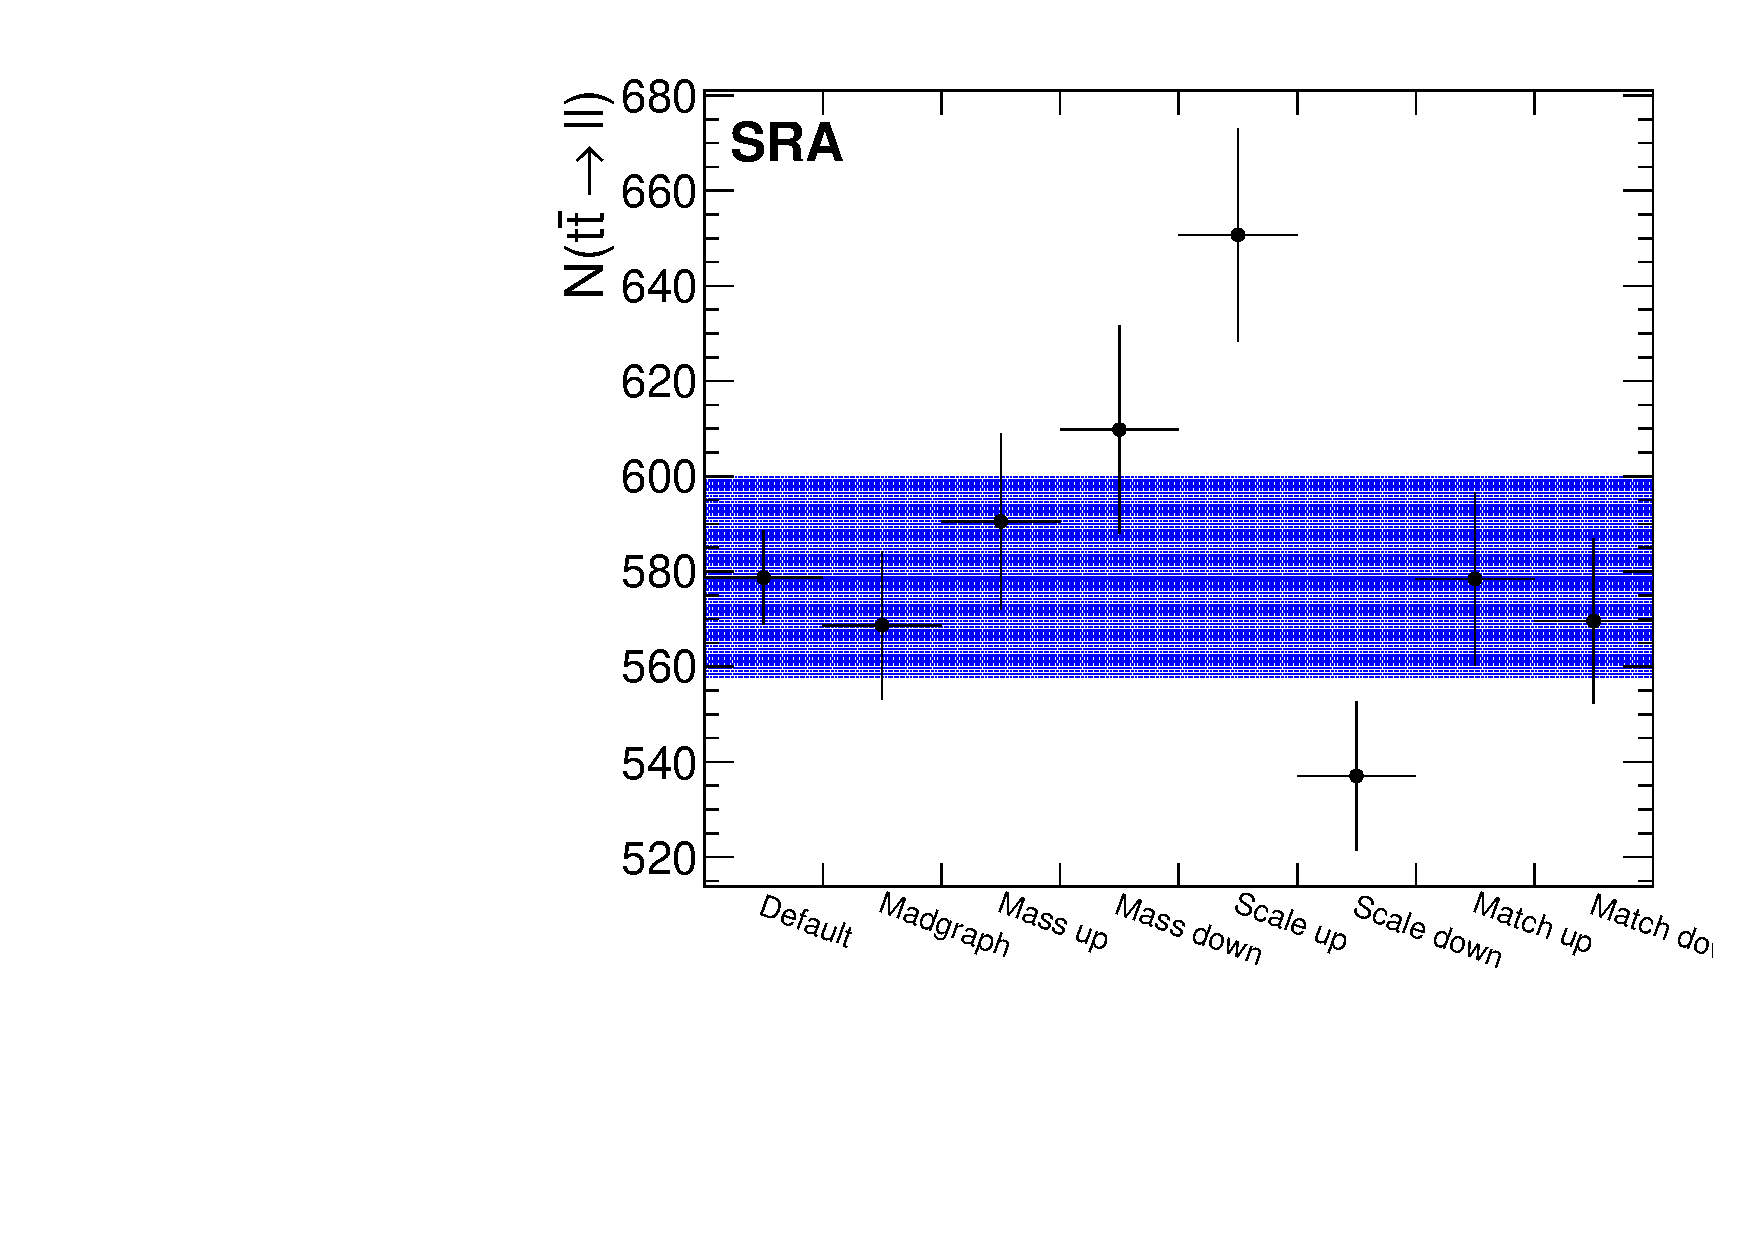
\includegraphics[width=0.5\linewidth]{plots/n_dl_comp_SRA.pdf}%
	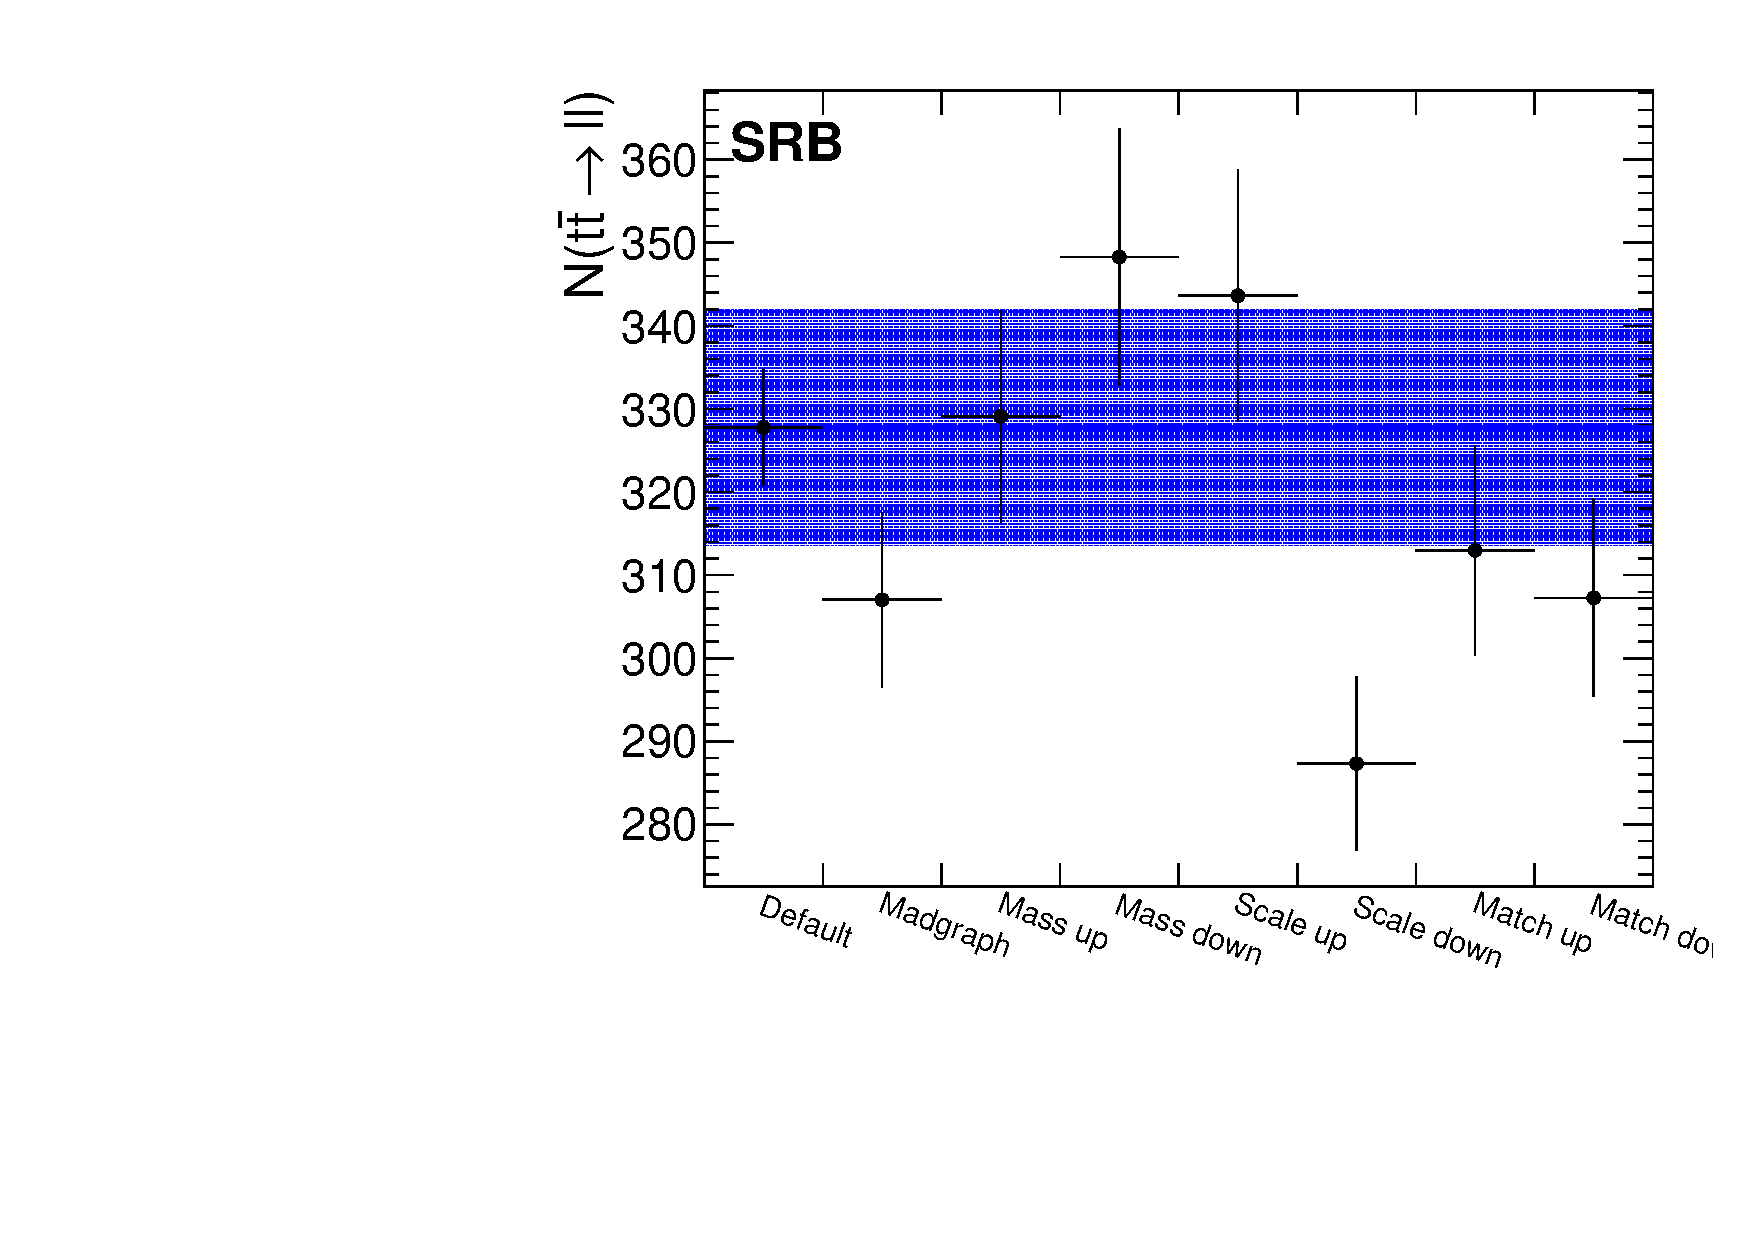
\includegraphics[width=0.5\linewidth]{plots/n_dl_comp_SRB.pdf}
	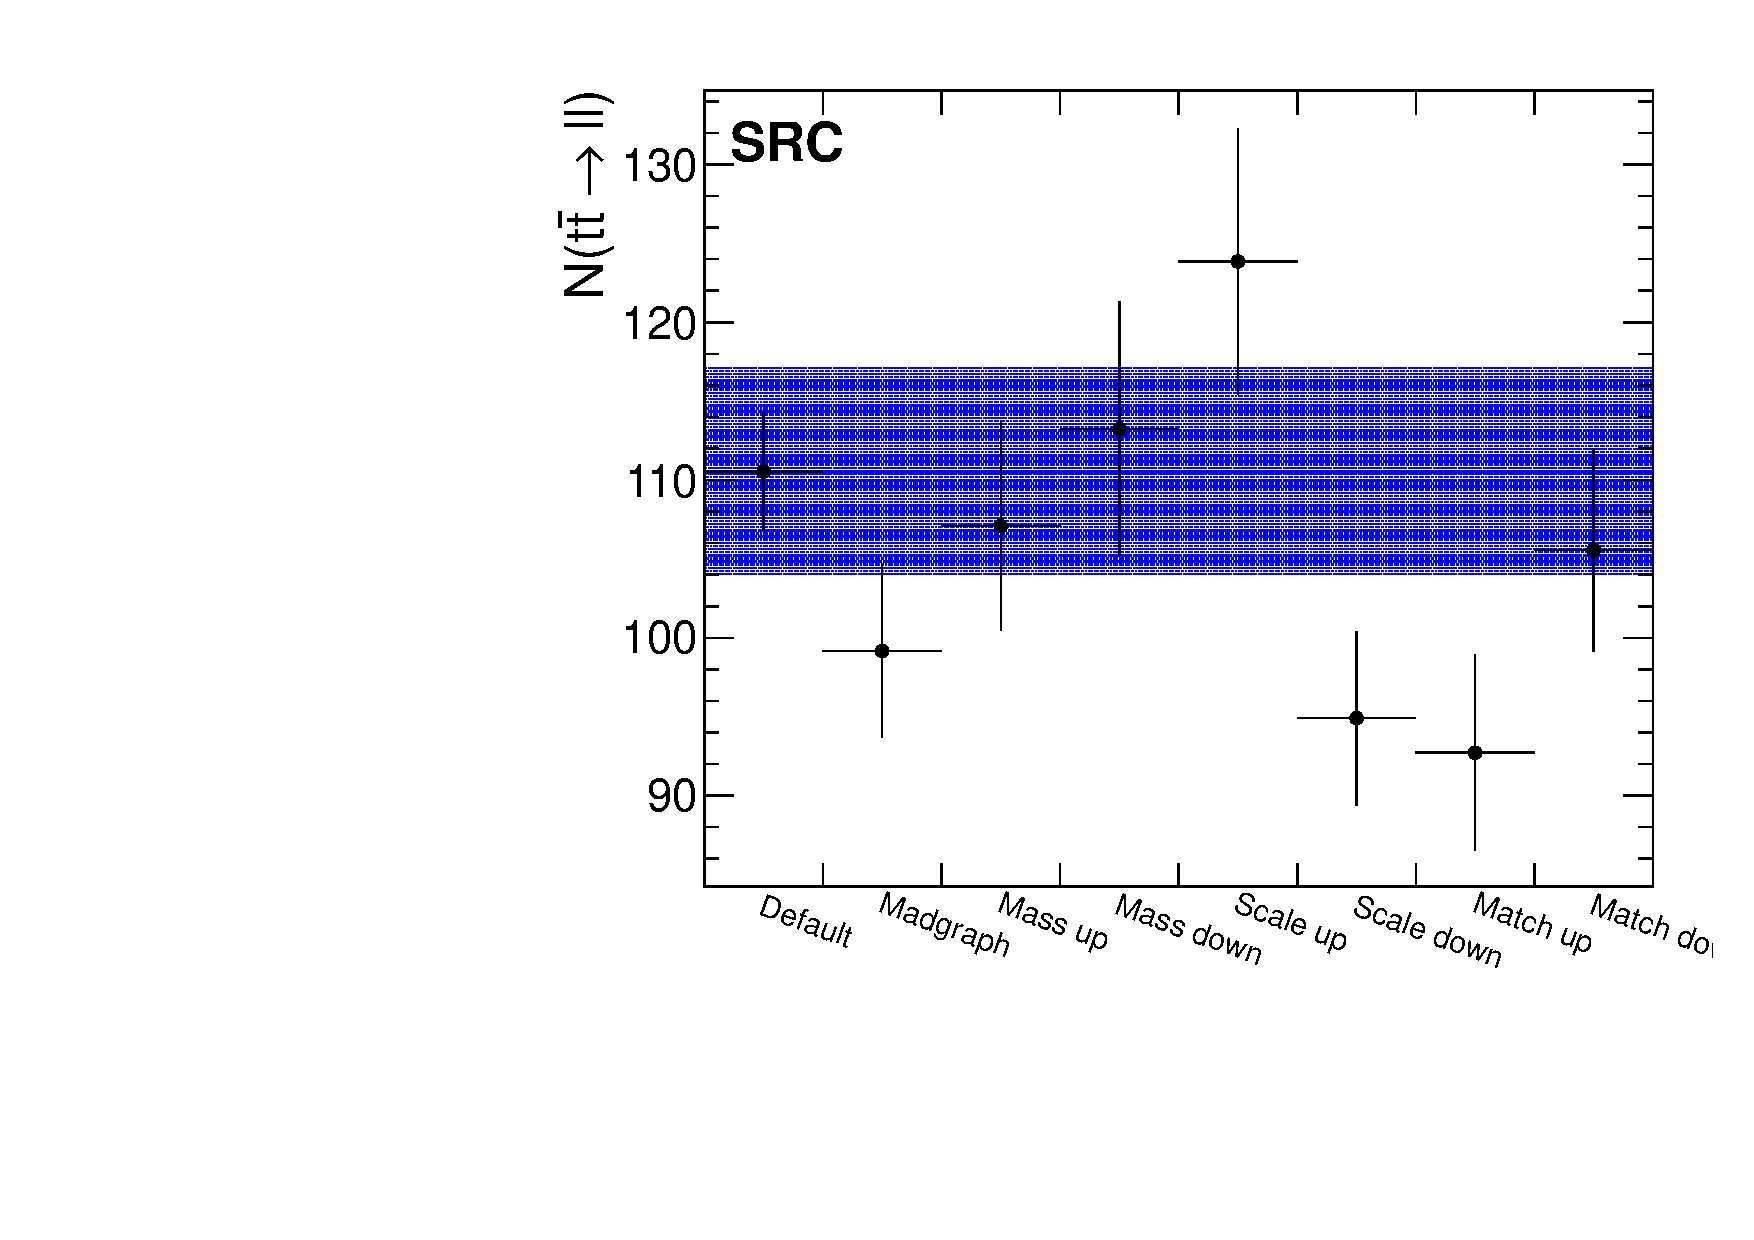
\includegraphics[width=0.5\linewidth]{plots/n_dl_comp_SRC.pdf}%
	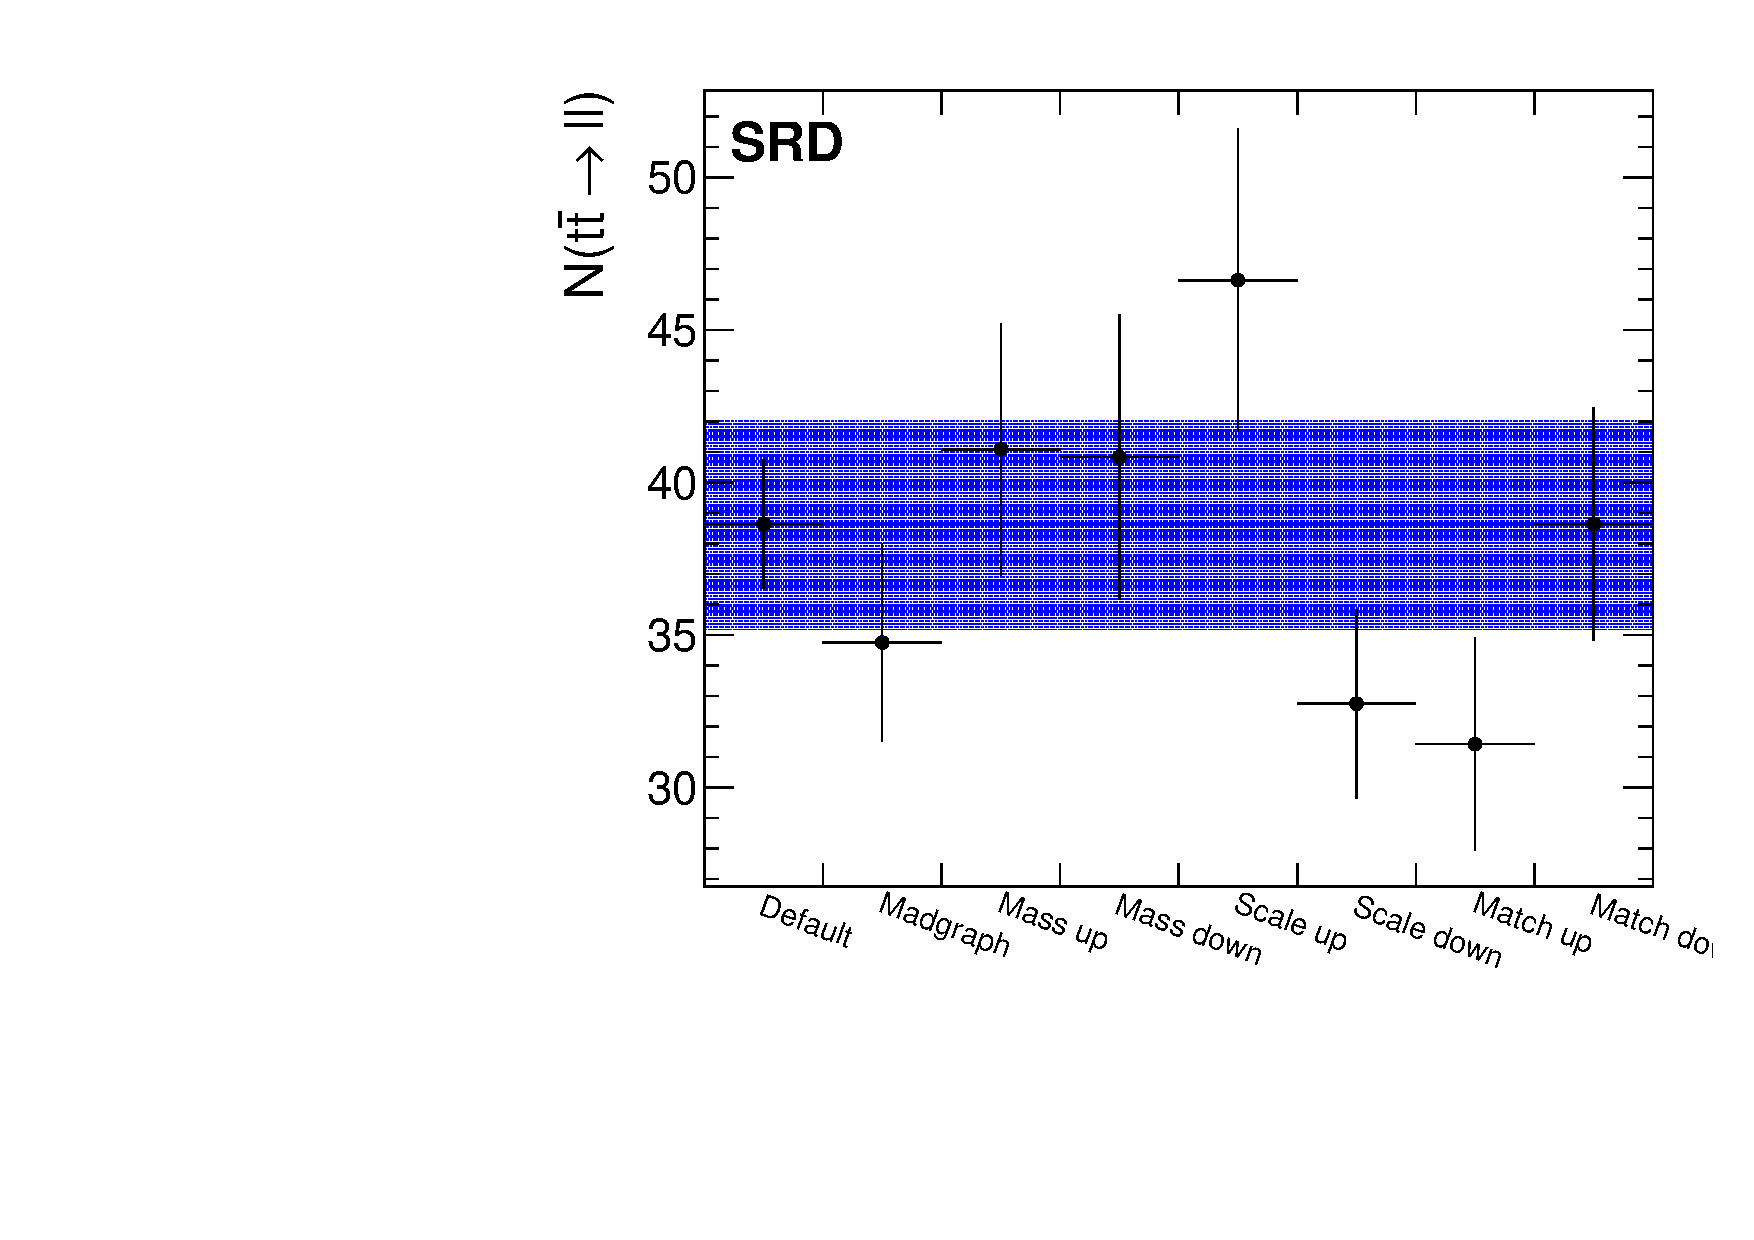
\includegraphics[width=0.5\linewidth]{plots/n_dl_comp_SRD.pdf}
	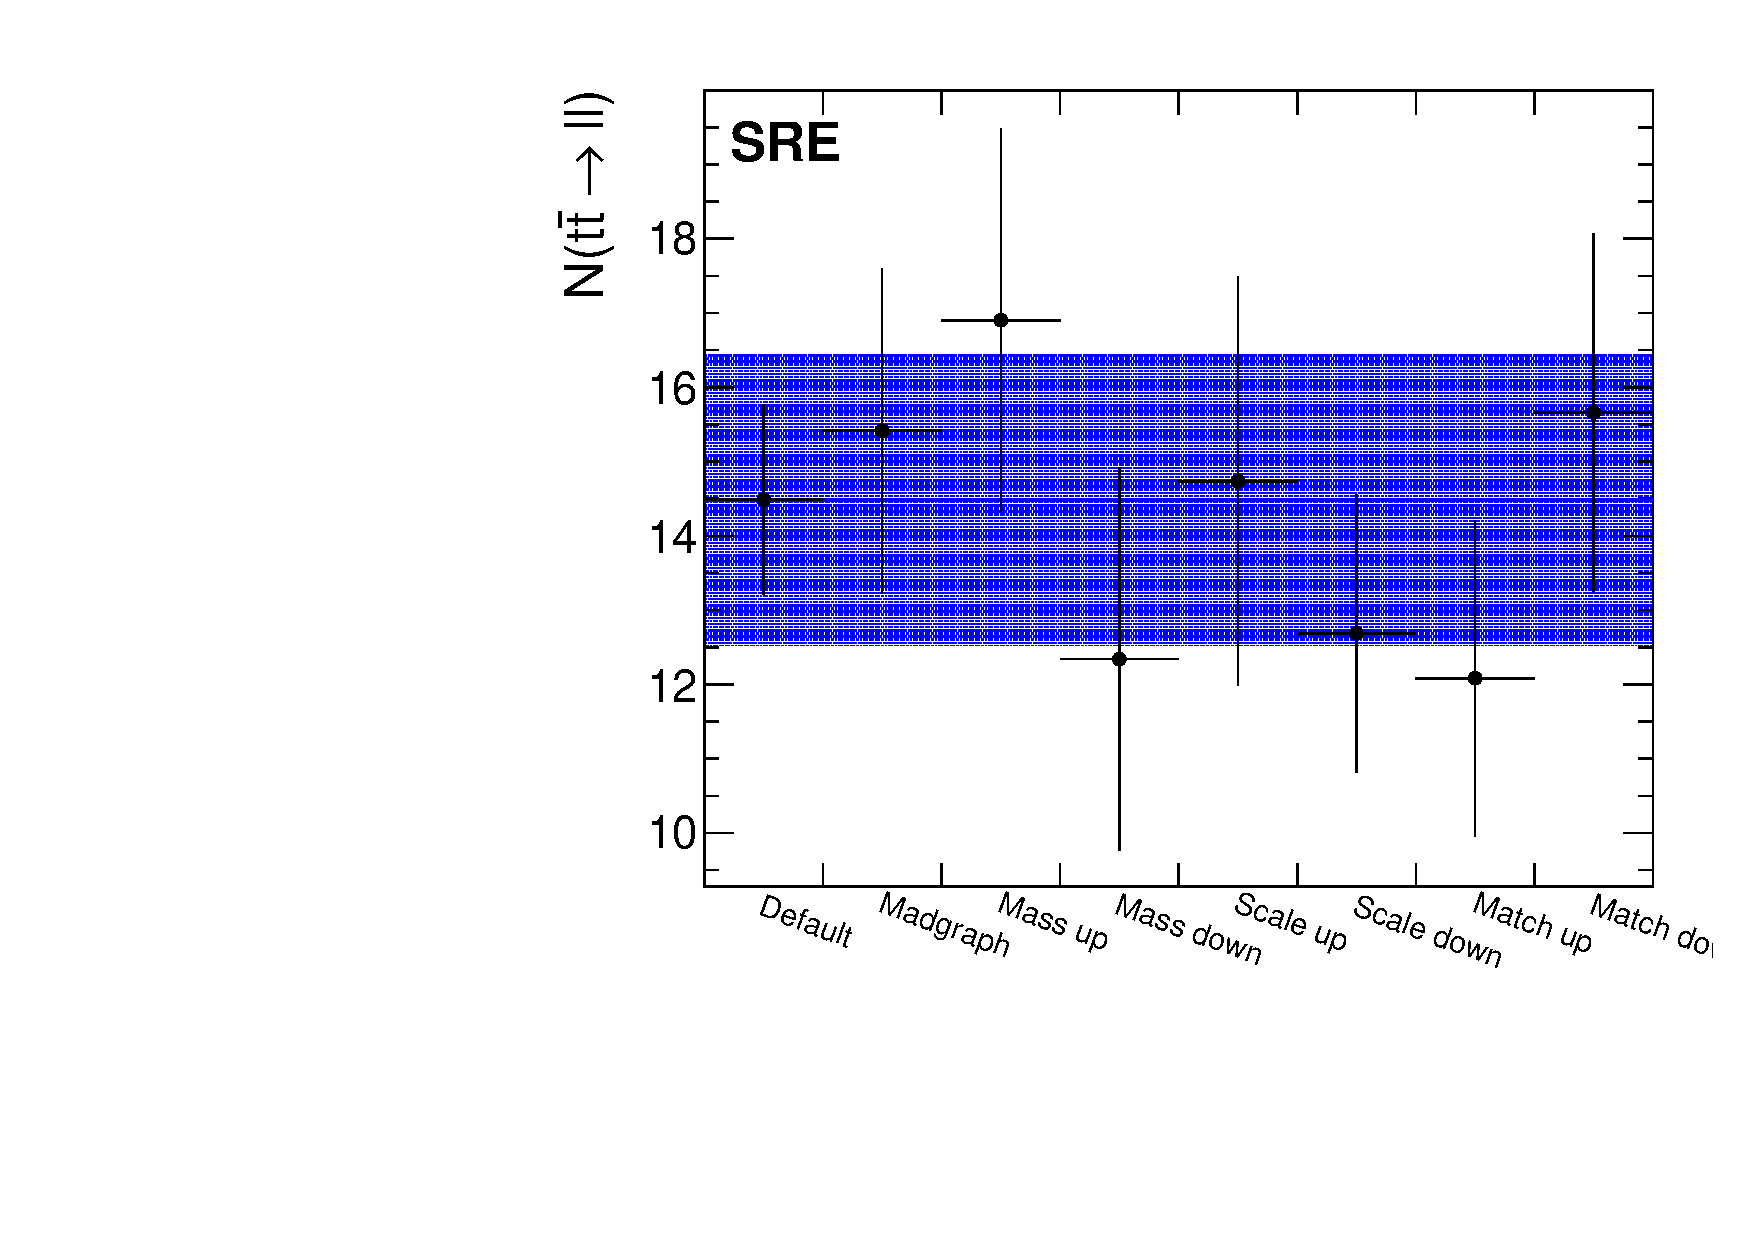
\includegraphics[width=0.5\linewidth]{plots/n_dl_comp_SRE.pdf}
	\caption{
	  \label{fig:ttllsyst}\protect 
          Comparison of the \ttll\ central prediction with those using
          alternative MC samples. The blue band corresponds to the
          total statistical error for all data and MC samples. The
          alternative sample predictions are indicated by the
          datapoints. The uncertainties on the alternative predictions
          correspond to the uncorrelated statistical uncertainty from
          the size of the alternative sample only.  Note the
          suppressed vertical scales.}
      \end{center}
    \end{figure}


\begin{table}[!h]
\begin{center}
{\footnotesize
\begin{tabular}{l||c|c|c|c|c|c|c}
\hline
$\Delta/N$  [\%] & Madgraph & Mass Up & Mass Down & Scale Up & Scale Down &
Match Up & Match Down \\
\hline
\hline
SRA 	 & $2$ & $2$ & $5$ & $12$ & $7$ & $0$ & $2$  \\
\hline
SRB 	 & $6$ & $0$ & $6$ & $5$ & $12$ & $5$ & $6$  \\
\hline
% SRC 	 & $10$ & $3$ & $2$ & $12$ & $14$ & $16$ & $4$  \\
% \hline
% SRD 	 & $10$ & $6$ & $6$ & $21$ & $15$ & $19$ & $0$  \\
% \hline
% SRE 	 & $6$ & $17$ & $15$ & $2$ & $12$ & $17$ & $8$  \\
\hline
\end{tabular}}
\caption{ Relative difference in \ttdl\ predictions for alternative MC
  samples in
the higher statistics regions SRA and SRB.  These differences 
are based on the central values of the predictions.  For a fuller
picture
of the situation, including statistical uncertainites, see Fig.~\ref{fig:ttllsyst}. 
\label{tab:fracdiff}}
\end{center}
\end{table}


In Fig.~\ref{fig:ttllsyst} we compare the alternate MC \ttll\ background predictions 
for regions A through E.  We can make the following observations based
on this Figure.

\begin{itemize}
\item In the tighter signal regions we are running out of
  statistics.    
\item Within the limited statistics, there is no evidence that the
  situation changes as we go from signal region A to signal region E.
%Therefore, we assess a systematic based on the relatively high
%statistics
%test in signal region A, and apply the same systematic uncertainty
%to all other regions.
\item In signal regions B and above, the uncertainties assigned in Section~\ref{sec:ttdilbkgunc}
fully cover the alternative MC variations.
\item In order to fully (as opposed as 1$\sigma$) cover the 
alternative MC variations in region A we would have to take a
systematic
uncertainty of $\approx 10\%$ instead of $5\%$.  This would be driven by the 
scale up/scale down variations, see Table~\ref{tab:fracdiff}.
\end{itemize}

\begin{table}[!ht]
\begin{center}
\begin{tabular}{l|c|c}
\hline
            Sample
            &                K3   & K4\\
\hline
\hline
Powheg     & $1.01 \pm 0.03$ & $0.93 \pm 0.04$ \\
Madgraph  & $1.01 \pm 0.04$ & $0.92 \pm 0.04$ \\
Mass Up    & $1.00 \pm 0.04$ & $0.92 \pm 0.04$ \\
Mass Down    & $1.06 \pm 0.04$ & $0.99 \pm 0.05$ \\
Scale Up    & $1.14 \pm 0.04$ & $1.23 \pm 0.06$ \\
Scale Down    & $0.89 \pm 0.03$ & $0.74 \pm 0.03$ \\
Match Up    & $1.02 \pm 0.04$ & $0.97 \pm 0.04$ \\
Match Down    & $1.02 \pm 0.04$ & $0.91 \pm 0.04$ \\
\hline
\end{tabular}
\caption{$\met>100$ GeV: Data/MC scale factors used to account for differences in the
  fraction of events with additional hard jets from radiation in
  \ttll\ events. \label{tab:njetskfactors_met100}}
\end{center}
\end{table}


However, we have two pieces of information indicating that the 
scale up/scale down variations are inconsistent with the data.
These are described below.

The first piece of information is that the jet multiplicity in the scale
up/scale down sample is the most inconsistent with the data.  This is shown
in Table~\ref{tab:njetskfactors_met100}, where we tabulate the
$K_3$ and $K_4$ factors of Section~\ref{sec:jetmultiplicity} for
different \ttbar\ MC samples.  The data/MC disagreement in the $N_{jets}$
distribution
for the scale up/scale down samples is also shown in Fig.~\ref{fig:dileptonnjets_scaleup}
and~\ref{fig:dileptonnjets_scaledw}.  This should be compared with the
equivalent $N_{jets}$ plots for the default Powheg MC, see 
Fig.~\ref{fig:dileptonnjets}, which agrees much better with data.

\begin{figure}[hbt]
  \begin{center}
        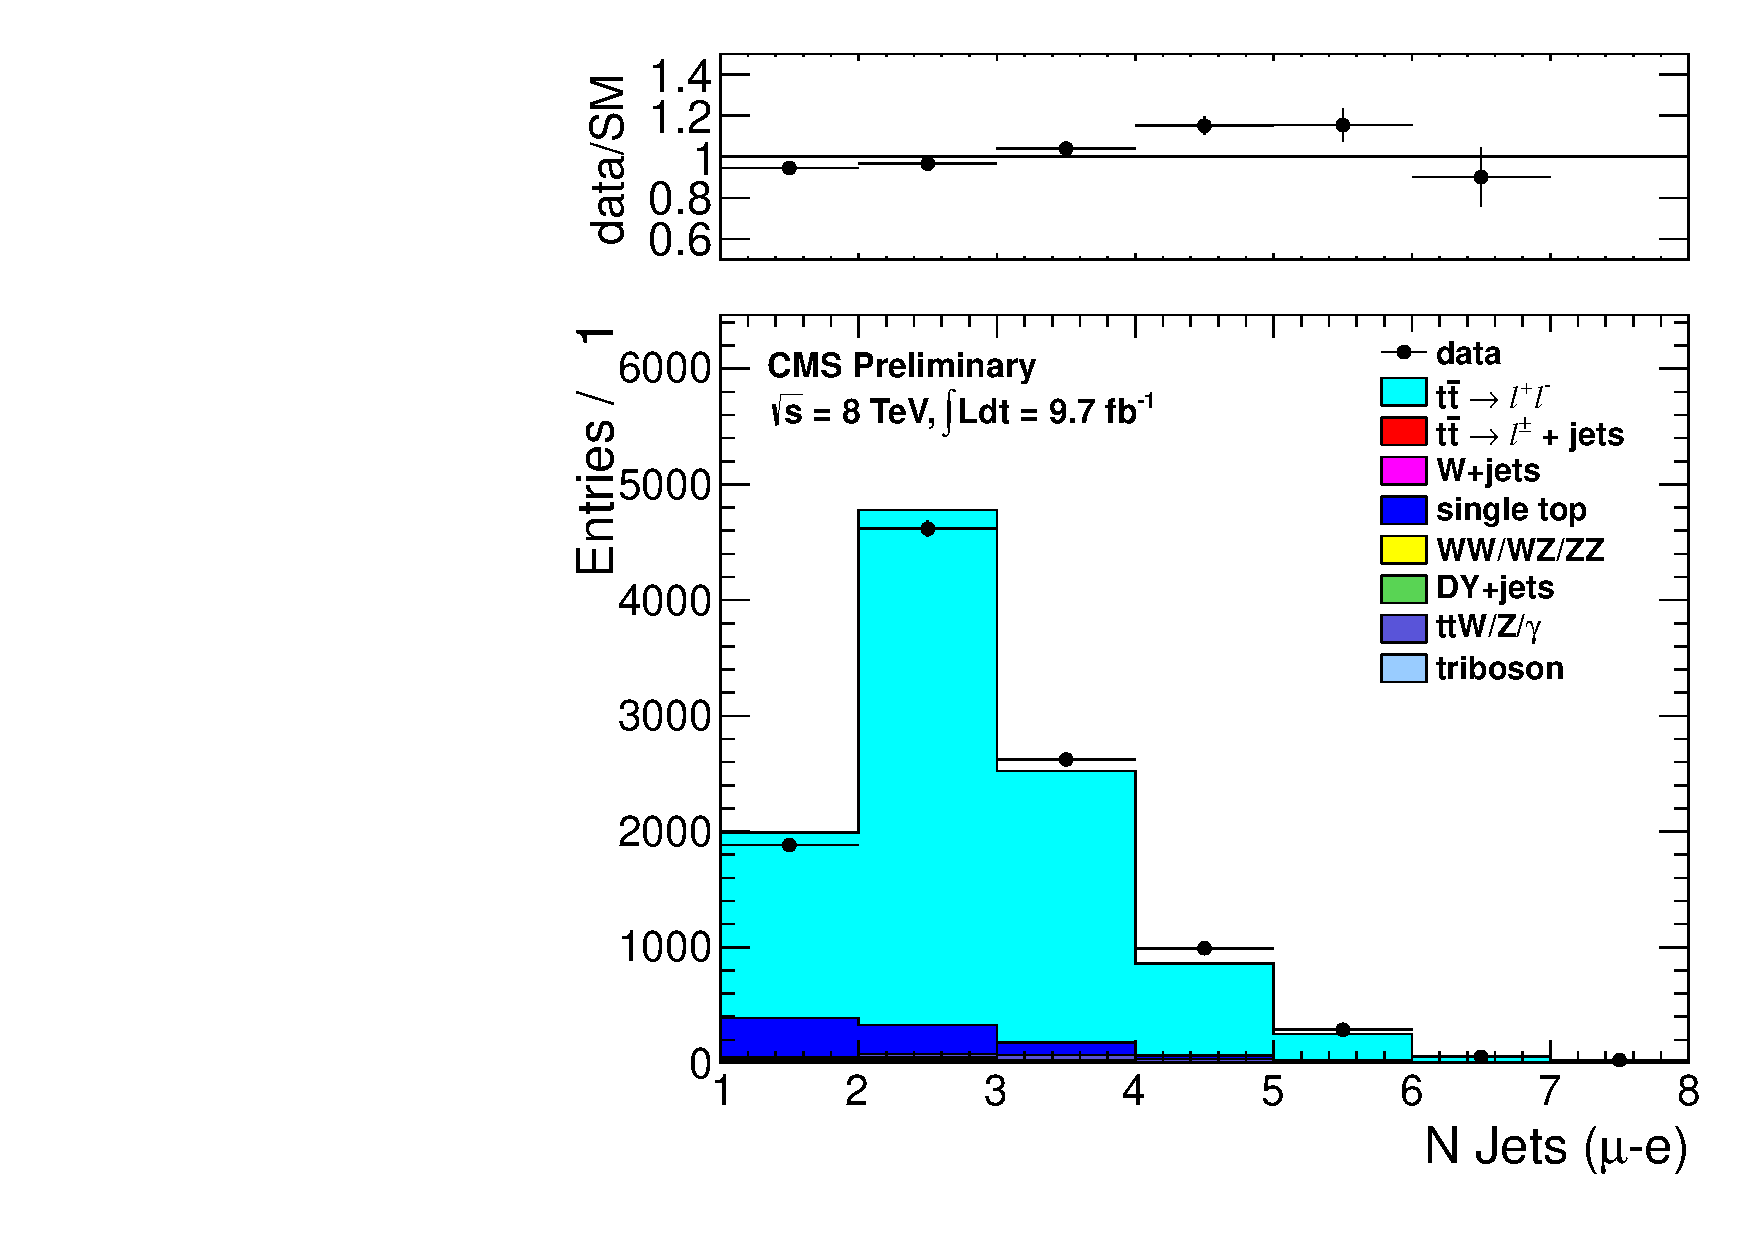
\includegraphics[width=0.5\linewidth]{plots/njets_all_met50_mueg_scaleup.pdf}
        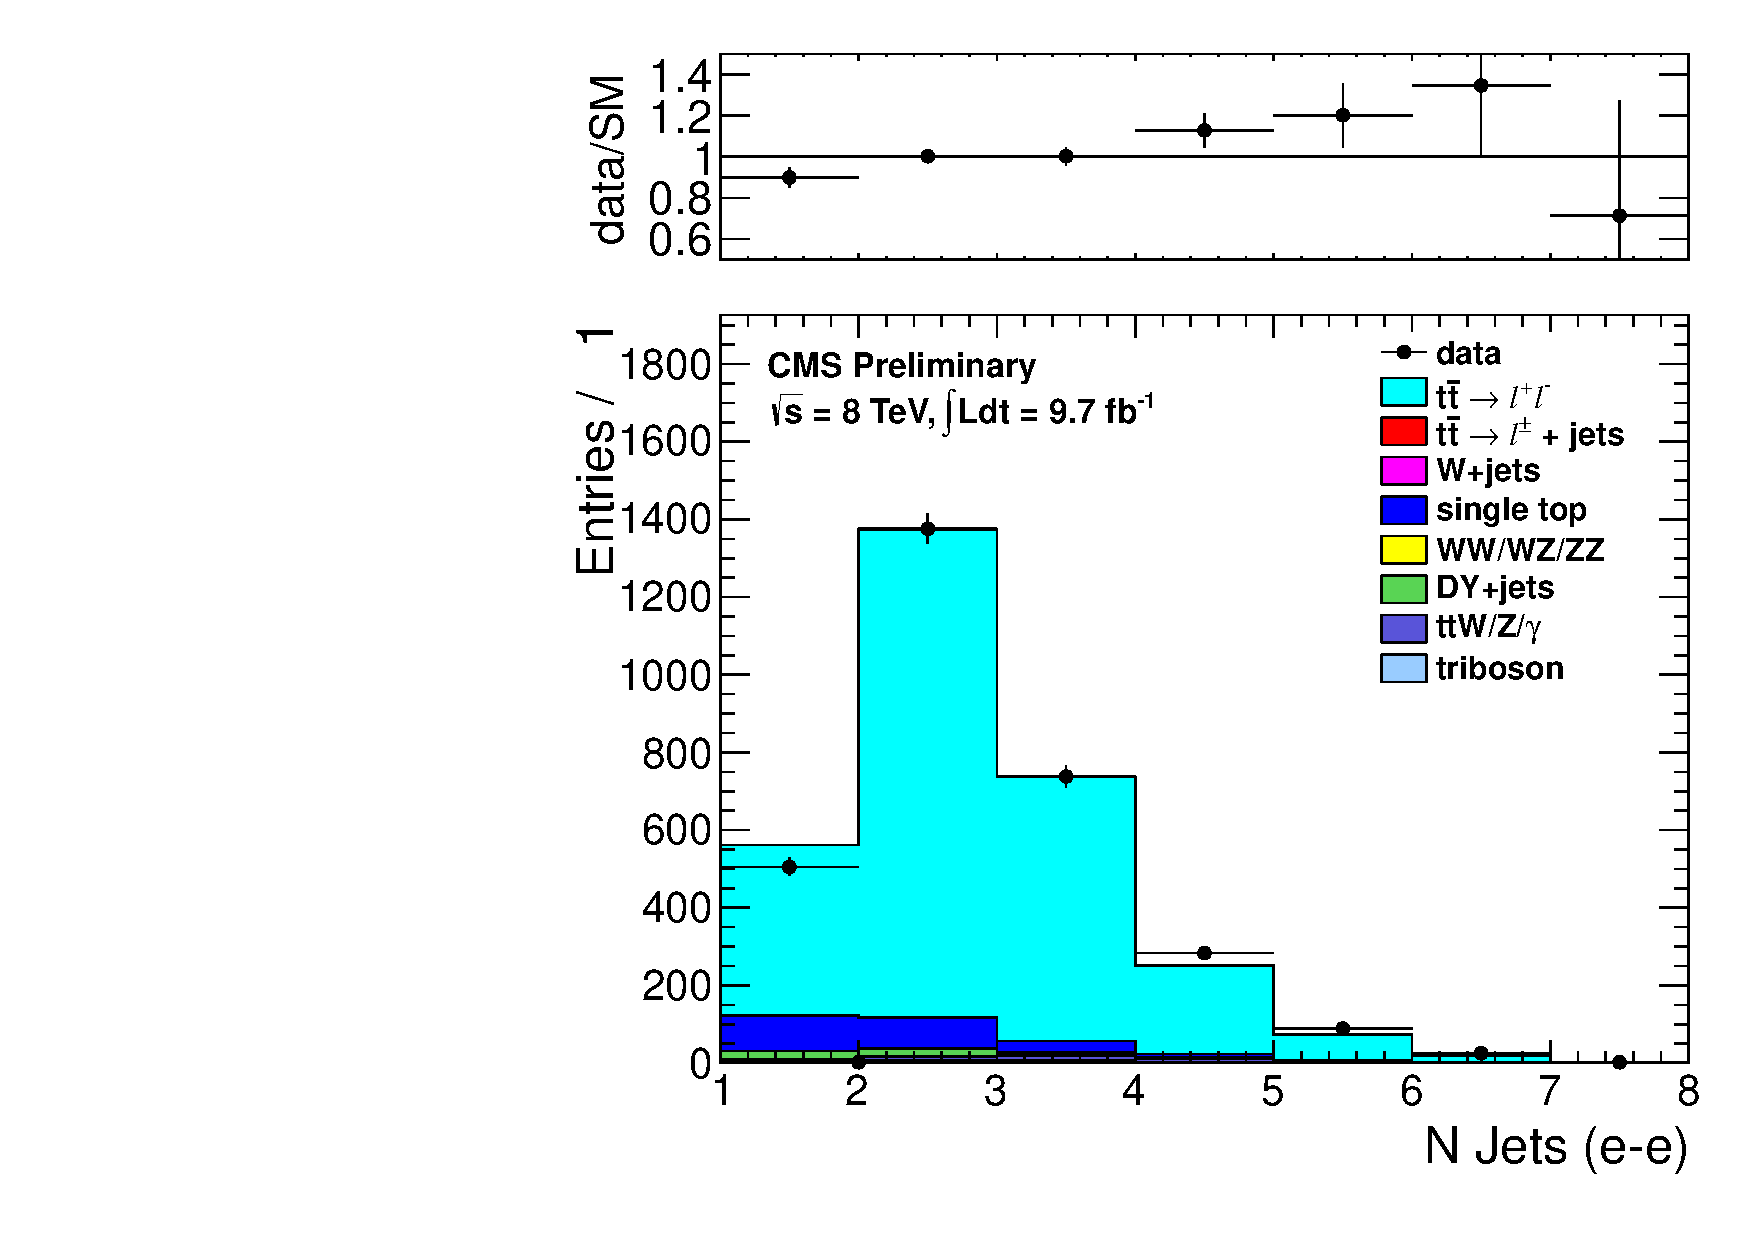
\includegraphics[width=0.5\linewidth]{plots/njets_all_met50_diel_scaleup.pdf}%
        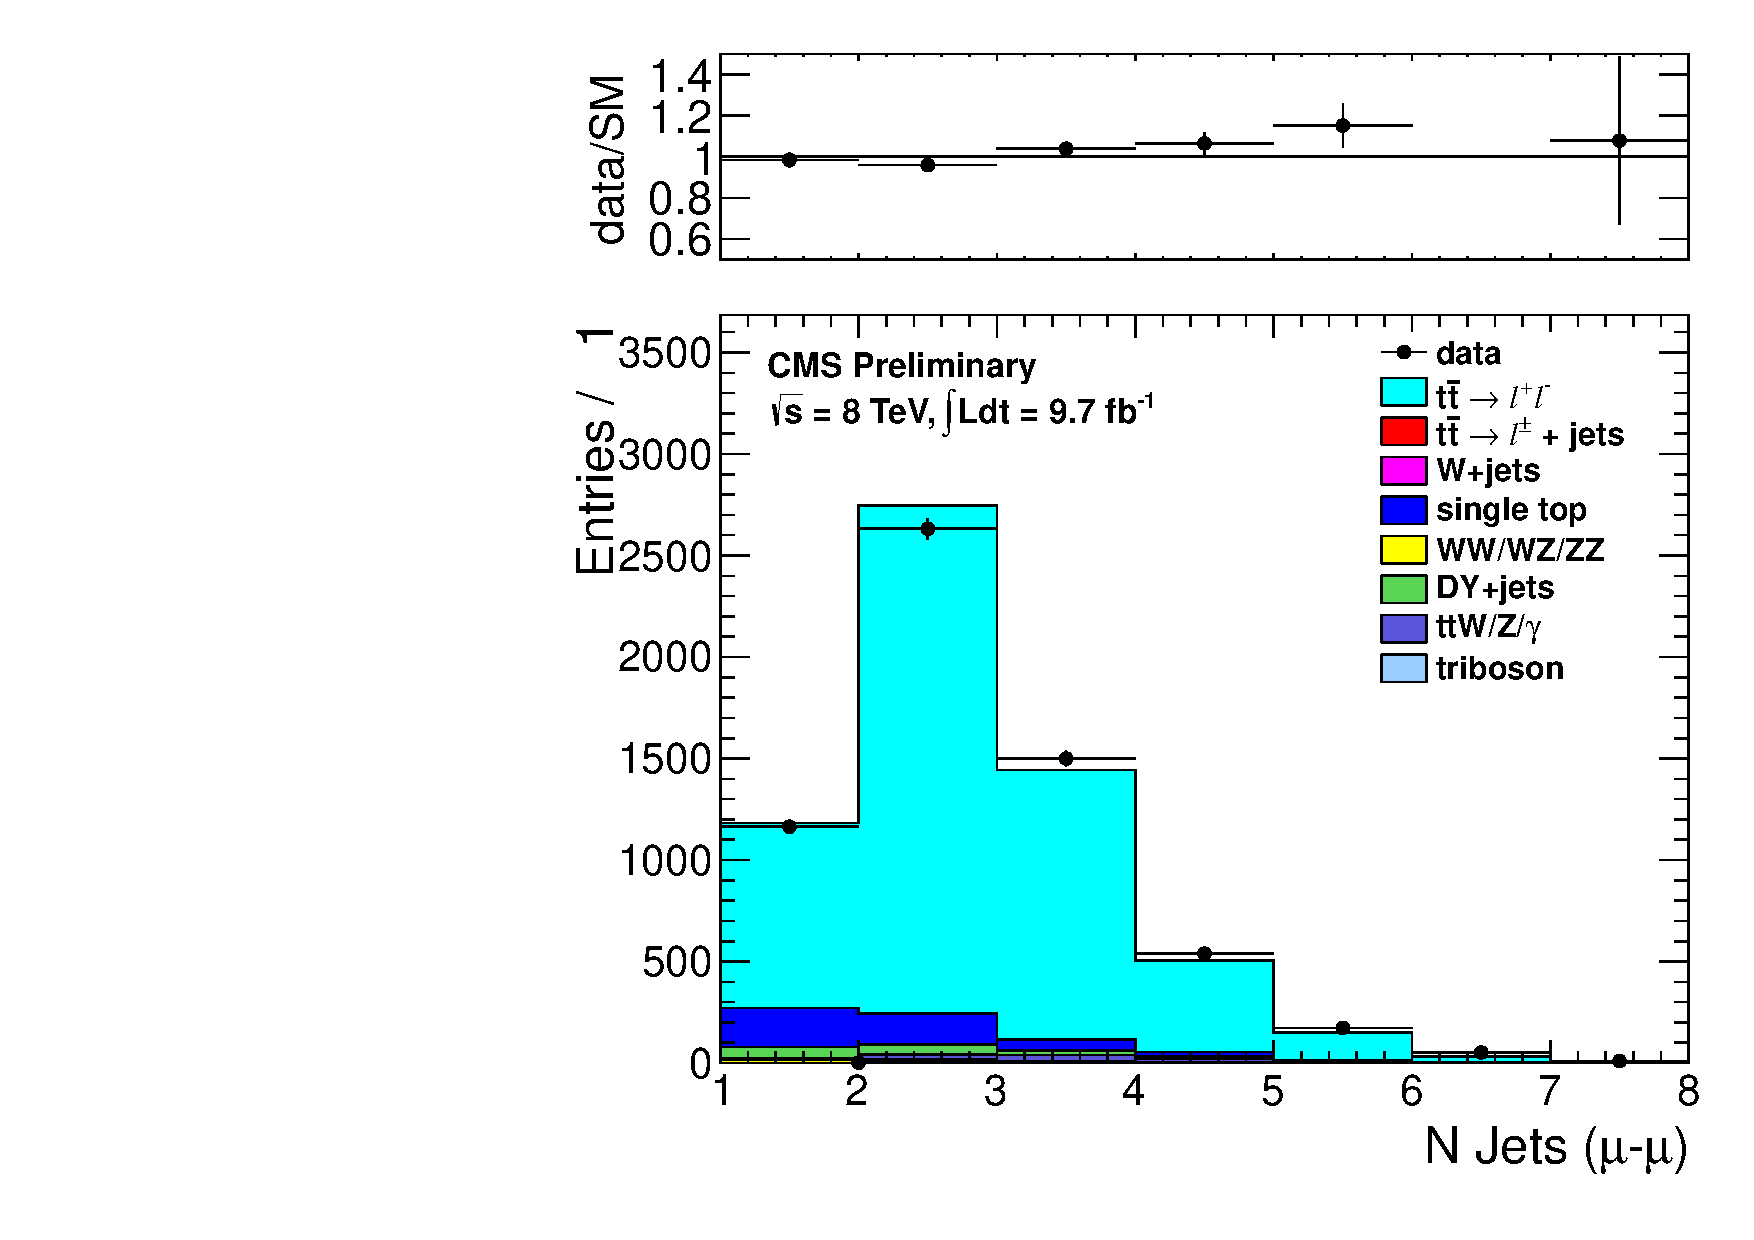
\includegraphics[width=0.5\linewidth]{plots/njets_all_met50_dimu_scaleup.pdf}
        \caption{
          \label{fig:dileptonnjets_scaleup}%\protect 
          SCALE UP: Comparison of the jet multiplicity distribution in data and MC for dilepton events in the \E-\M\
          (top), \E-\E\ (bottom left) and \M-\M\ (bottom right) channels.}  
      \end{center}
\end{figure}

\begin{figure}[hbt]
  \begin{center}
        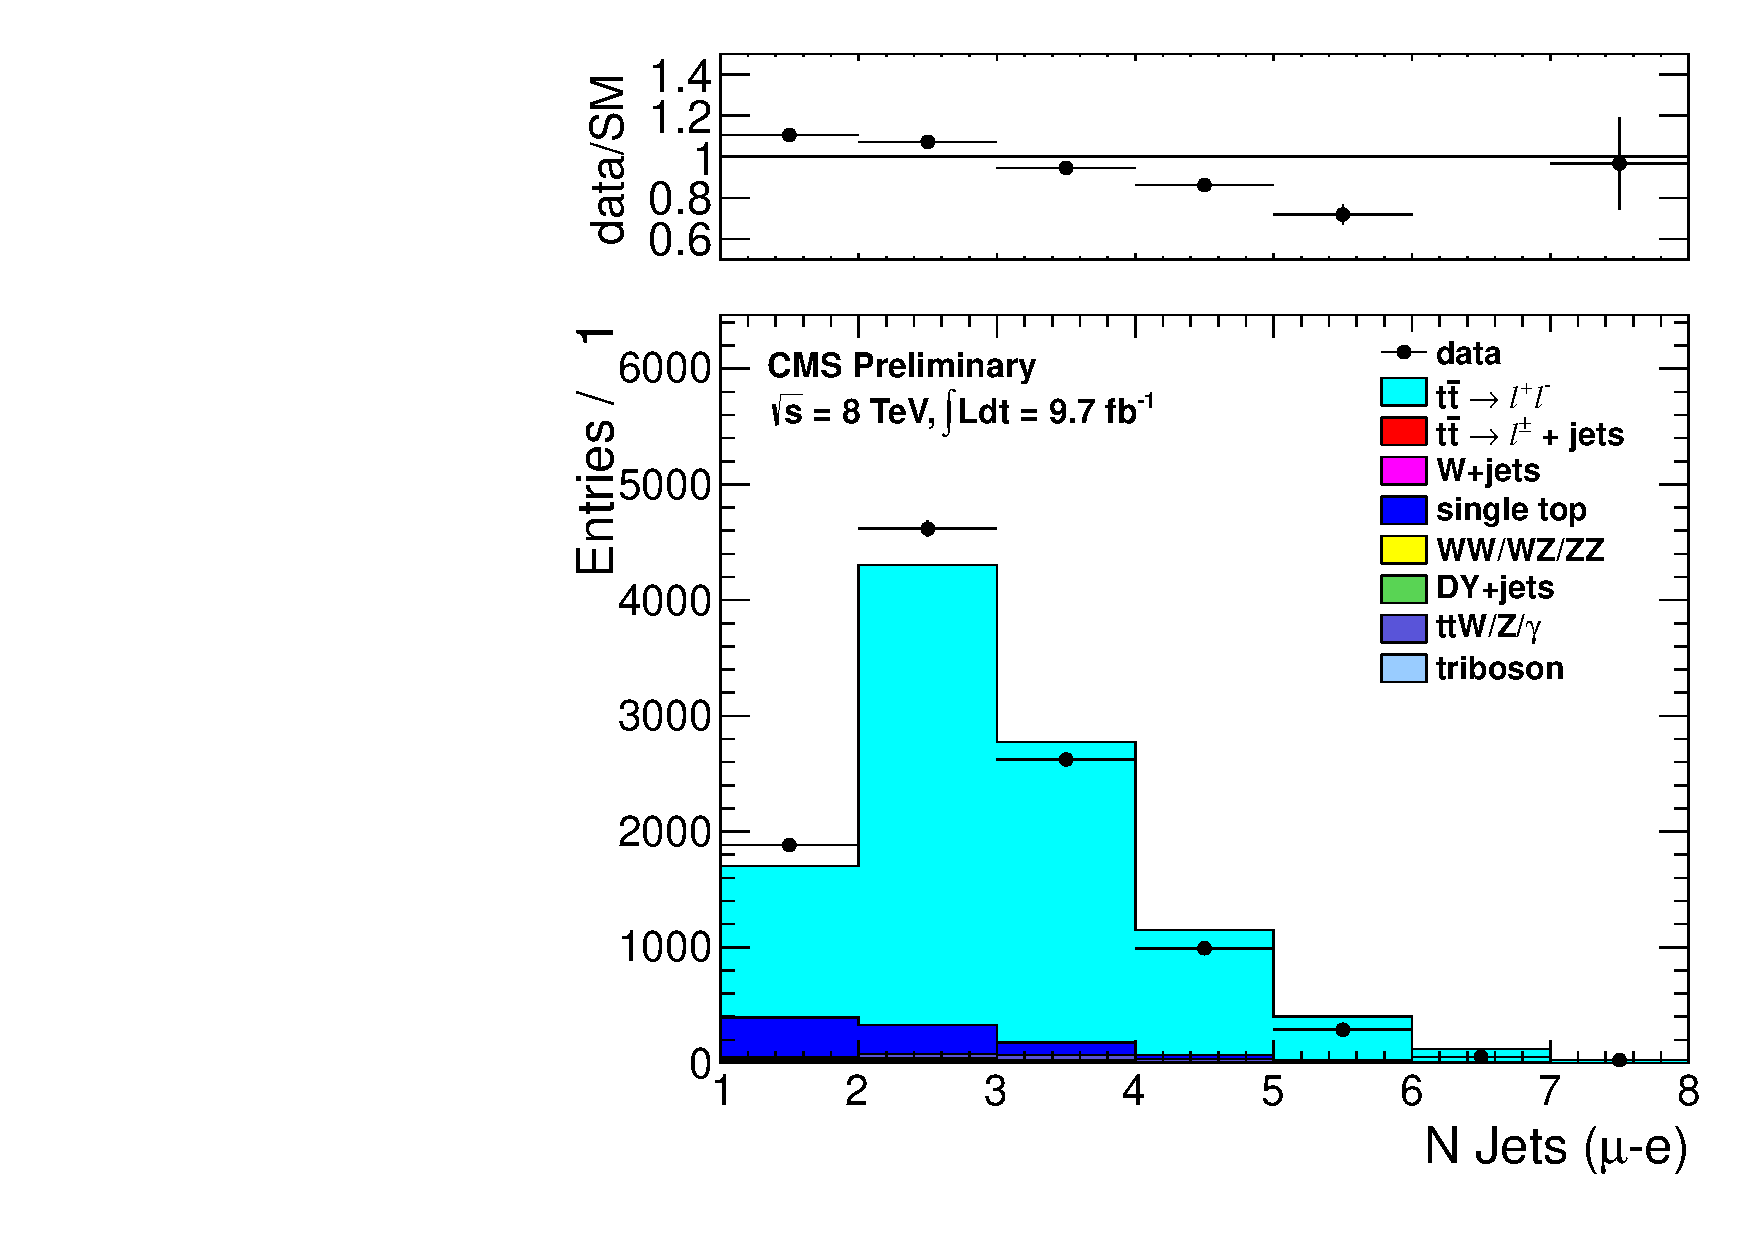
\includegraphics[width=0.5\linewidth]{plots/njets_all_met50_mueg_scaledw.pdf}
        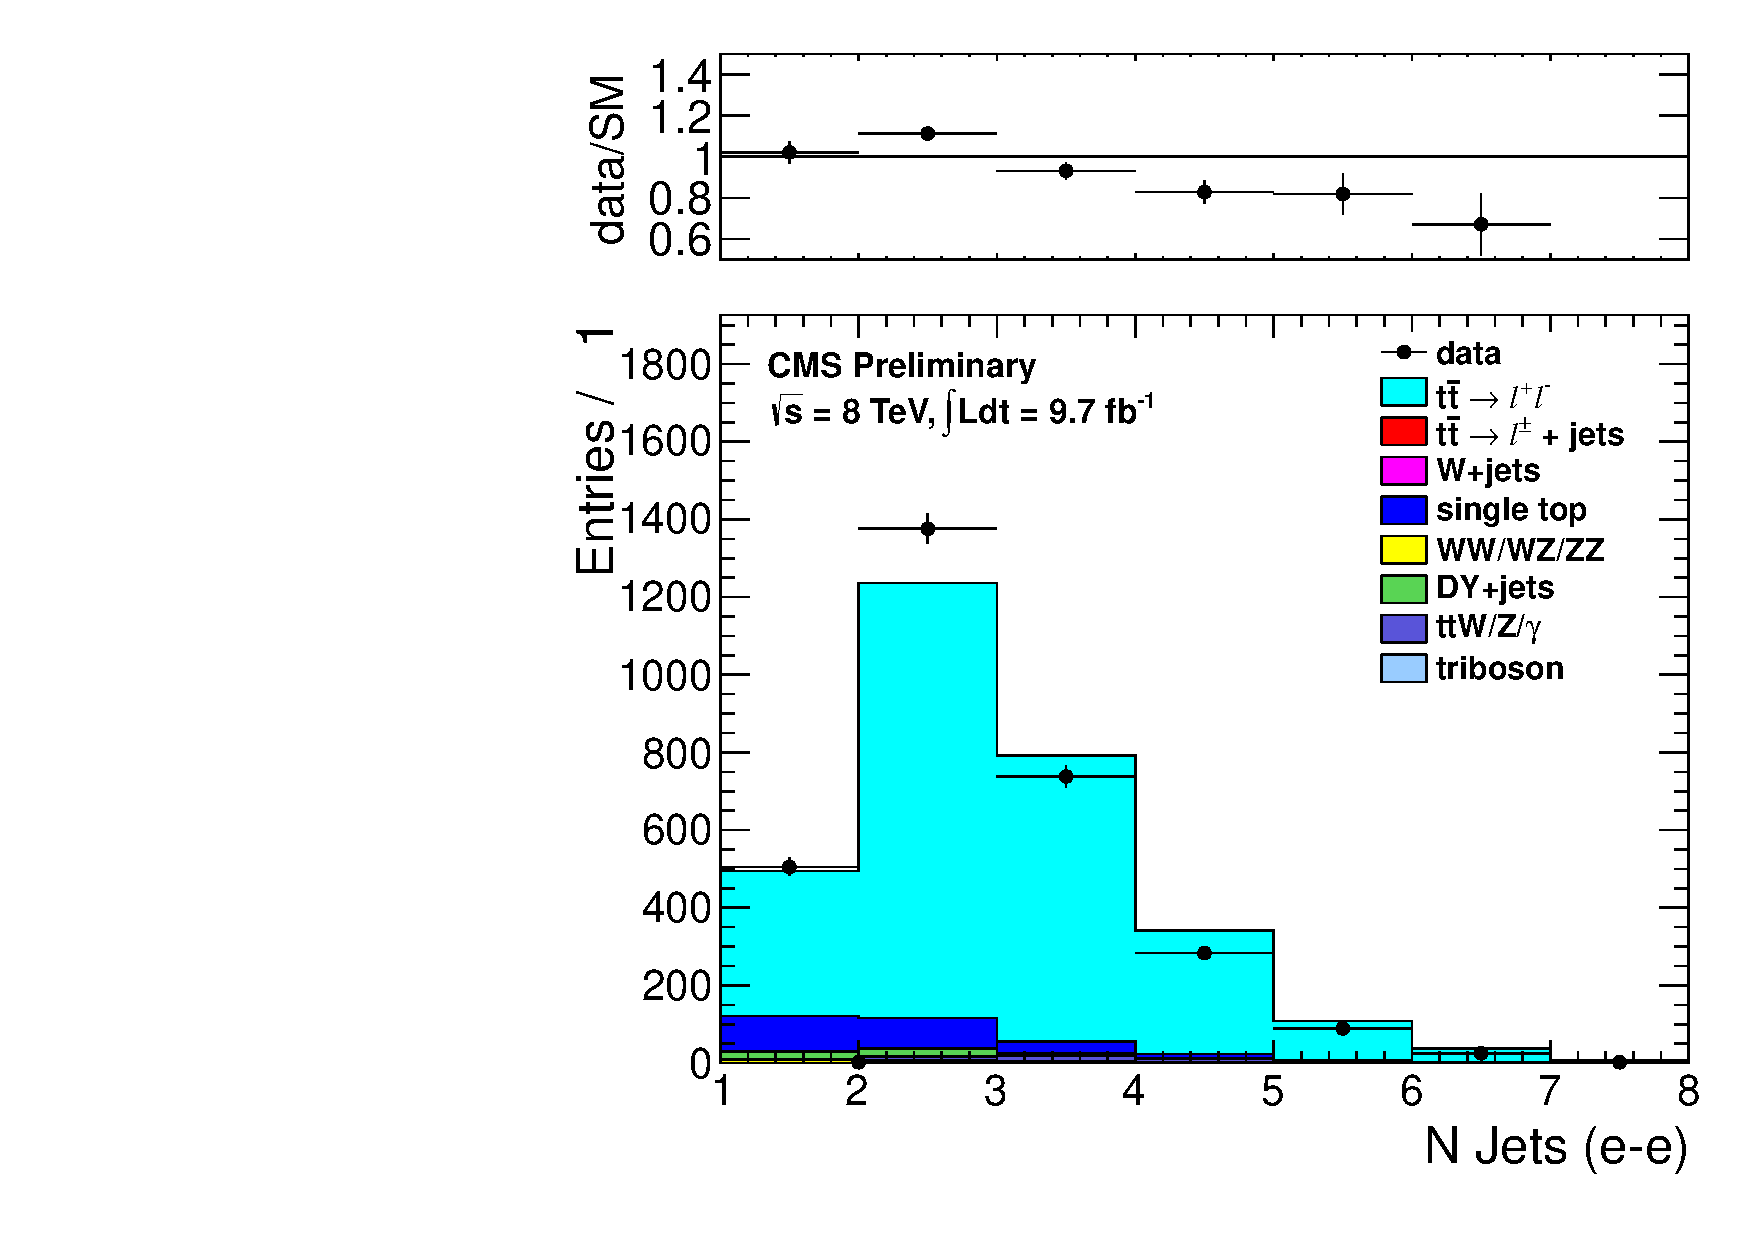
\includegraphics[width=0.5\linewidth]{plots/njets_all_met50_diel_scaledw.pdf}%
        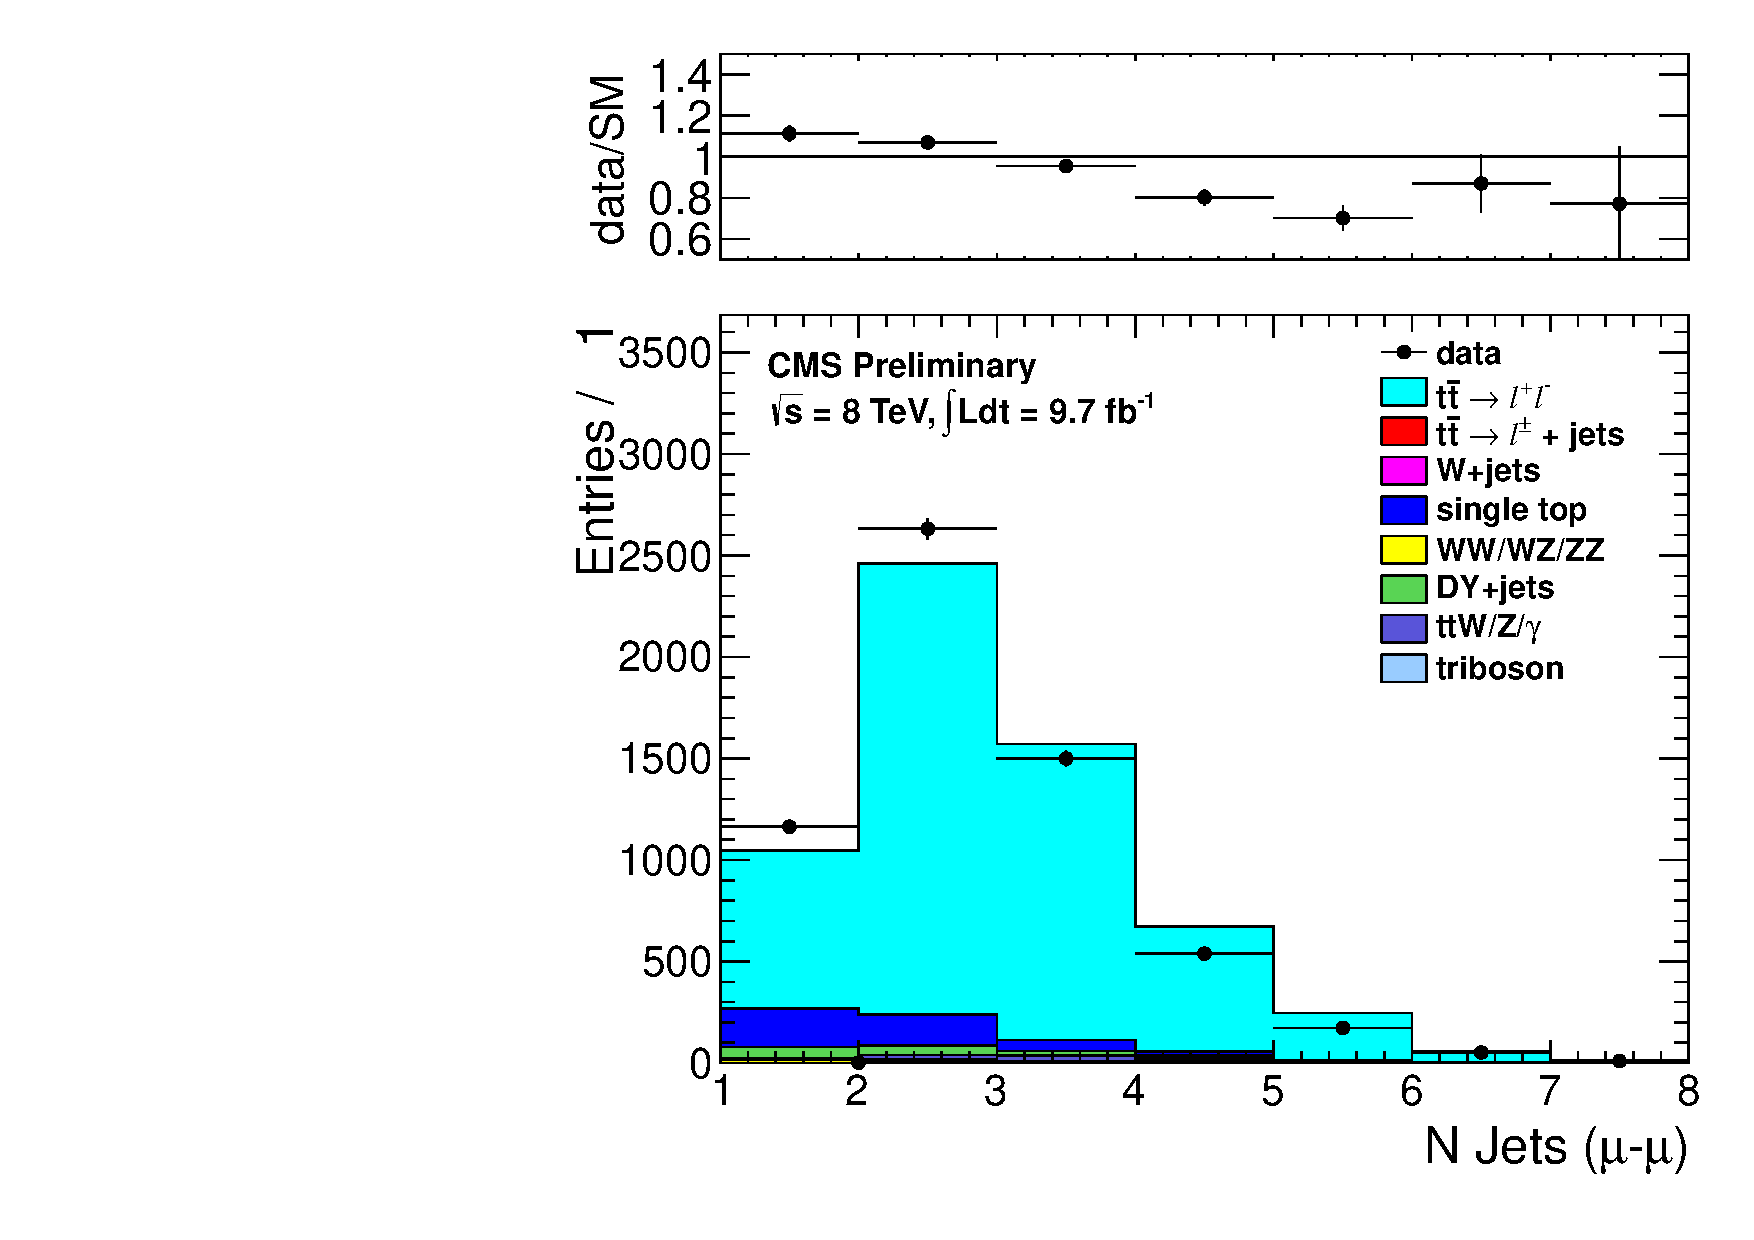
\includegraphics[width=0.5\linewidth]{plots/njets_all_met50_dimu_scaledw.pdf}
        \caption{
          \label{fig:dileptonnjets_scaledw}%\protect 
          SCALE DOWN: Comparison of the jet multiplicity distribution in data and MC for dilepton events in the \E-\M\
          (top), \E-\E\ (bottom left) and \M-\M\ (bottom right) channels.}  
      \end{center}
\end{figure}


\clearpage

The second piece of information is that we have performed closure
tests in CR5 using the alternative MC samples.  These are exactly
the same tests as the one performed in Section~\ref{sec:CR5} on the
Powheg sample.  As we argued previously, this is a very powerful 
test of the background calculation.
The results of this test are summarized in Table~\ref{tab:hugecr5yields}.
Concentrating on the relatively high statistics CR5A region, we see
for all \ttbar\ MC samples except scale up/scale down we obtain
closure within 1$\sigma$.  The scale up/scale down tests closes
worse, only within 2$\sigma$.  This again is evidence that the 
scale up/scale down variations are in disagreement with the data.


\begin{table}[!h]
\begin{center}
{\footnotesize
\begin{tabular}{l||c||c|c|c|c|c}
\hline
Sample              & CR5PRESEL & CR5A & CR5B & CR5C & CR5D & CR5E\\
\hline
\hline
\multicolumn{7}{c}{POWHEG} \\
%\hline
%$\mu$ MC 		  & $490 \pm 9$ & $299 \pm 7$ & $155 \pm 6$ & $49 \pm 3$ & $19 \pm 2$ & $7 \pm 1$ \\
%$\mu$ Data 		  & $514$ & $311$ & $167$ & $57$ & $12$ & $4$ \\
\hline
$\mu$ Data/MC SF 	  & $1.05 \pm 0.05$ & $1.04 \pm 0.06$ & $1.08 \pm 0.09$ & $1.17 \pm 0.17$ & $0.64 \pm 0.20$ & $0.54 \pm 0.29$ \\
%\hline
%e MC 		  & $405 \pm 8$ & $239 \pm 7$ & $130 \pm 5$ & $43 \pm 3$ & $16 \pm 2$ & $8 \pm 1$ \\
%e Data 		  & $427$ & $248$ & $120$ & $38$ & $14$ & $4$ \\
\hline
e Data/MC SF 	  & $1.06 \pm 0.06$ & $1.04 \pm 0.07$ & $0.93 \pm 0.09$ & $0.89 \pm 0.16$ & $0.86 \pm 0.25$ & $0.52 \pm 0.28$ \\
%\hline
%$\mu$+e MC 		  & $894 \pm 12$ & $538 \pm 10$ & $284 \pm 8$ & $92 \pm 4$ & $35 \pm 3$ & $15 \pm 2$ \\
%$\mu$+e Data 		  & $941$ & $559$ & $287$ & $95$ & $26$ & $8$ \\
\hline
$\mu$+e Data/MC SF 		  & $1.05 \pm 0.04$ & $1.04 \pm 0.05$ & $1.01 \pm 0.07$ & $1.04 \pm 0.12$ & $0.74 \pm 0.16$ & $0.53 \pm 0.20$ \\
\hline
\hline
\multicolumn{7}{c}{MADGRAPH} \\
%\hline
%$\mu$ MC 		  & $487 \pm 12$ & $293 \pm 10$ & $154 \pm 8$ & $47 \pm 4$ & $19 \pm 3$ & $9 \pm 2$ \\
%$\mu$ Data 		  & $514$ & $311$ & $167$ & $57$ & $12$ & $4$ \\
\hline
$\mu$ Data/MC SF 	  & $1.05 \pm 0.05$ & $1.06 \pm 0.07$ & $1.08 \pm 0.10$ & $1.21 \pm 0.19$ & $0.64 \pm 0.21$ & $0.43 \pm 0.24$ \\
%\hline
%e MC 		  & $401 \pm 11$ & $237 \pm 9$ & $124 \pm 7$ & $39 \pm 4$ & $13 \pm 2$ & $6 \pm 1$ \\
%e Data 		  & $427$ & $248$ & $120$ & $38$ & $14$ & $4$ \\
\hline
e Data/MC SF 	  & $1.06 \pm 0.06$ & $1.04 \pm 0.08$ & $0.97 \pm 0.10$ & $0.97 \pm 0.18$ & $1.10 \pm 0.34$ & $0.68 \pm 0.38$ \\
%\hline
%$\mu$+e MC 		  & $889 \pm 17$ & $530 \pm 13$ & $278 \pm 10$ & $86 \pm 5$ & $31 \pm 3$ & $15 \pm 2$ \\
%$\mu$+e Data 		  & $941$ & $559$ & $287$ & $95$ & $26$ & $8$ \\
\hline
$\mu$+e Data/MC SF 		  & $1.06 \pm 0.04$ & $1.05 \pm 0.05$ & $1.03 \pm 0.07$ & $1.10 \pm 0.13$ & $0.83 \pm 0.18$ & $0.53 \pm 0.21$ \\
\hline
\hline
\multicolumn{7}{c}{MASS UP} \\
%\hline
%$\mu$ MC 		  & $492 \pm 14$ & $300 \pm 11$ & $156 \pm 8$ & $48 \pm 4$ & $21 \pm 3$ & $7 \pm 2$ \\
%$\mu$ Data 		  & $514$ & $311$ & $167$ & $57$ & $12$ & $4$ \\
\hline
$\mu$ Data/MC SF 	  & $1.04 \pm 0.06$ & $1.04 \pm 0.07$ & $1.07 \pm 0.10$ & $1.20 \pm 0.19$ & $0.57 \pm 0.18$ & $0.56 \pm 0.31$ \\
%\hline
%e MC 		  & $410 \pm 13$ & $236 \pm 10$ & $119 \pm 7$ & $34 \pm 4$ & $14 \pm 2$ & $7 \pm 2$ \\
%e Data 		  & $427$ & $248$ & $120$ & $38$ & $14$ & $4$ \\
\hline
e Data/MC SF 	  & $1.04 \pm 0.06$ & $1.05 \pm 0.08$ & $1.01 \pm 0.11$ & $1.12 \pm 0.22$ & $1.02 \pm 0.33$ & $0.61 \pm 0.34$ \\
%\hline
%$\mu$+e MC 		  & $902 \pm 19$ & $536 \pm 15$ & $275 \pm 11$ & $81 \pm 6$ & $35 \pm 4$ & $14 \pm 2$ \\
%$\mu$+e Data 		  & $941$ & $559$ & $287$ & $95$ & $26$ & $8$ \\
\hline
$\mu$+e Data/MC SF 		  & $1.04 \pm 0.04$ & $1.04 \pm 0.05$ & $1.04 \pm 0.07$ & $1.17 \pm 0.15$ & $0.74 \pm 0.17$ & $0.58 \pm 0.23$ \\
\hline
\hline
\multicolumn{7}{c}{MASS DOWN} \\
%\hline
%$\mu$ MC 		  & $504 \pm 16$ & $304 \pm 13$ & $160 \pm 10$ & $45 \pm 5$ & $15 \pm 3$ & $4 \pm 1$ \\
%$\mu$ Data 		  & $514$ & $311$ & $167$ & $57$ & $12$ & $4$ \\
\hline
$\mu$ Data/MC SF 	  & $1.02 \pm 0.06$ & $1.02 \pm 0.07$ & $1.04 \pm 0.10$ & $1.25 \pm 0.21$ & $0.82 \pm 0.28$ & $0.94 \pm 0.56$ \\
%\hline
%e MC 		  & $403 \pm 15$ & $242 \pm 12$ & $126 \pm 9$ & $42 \pm 5$ & $13 \pm 2$ & $7 \pm 2$ \\
%e Data 		  & $427$ & $248$ & $120$ & $38$ & $14$ & $4$ \\
\hline
e Data/MC SF 	  & $1.06 \pm 0.06$ & $1.02 \pm 0.08$ & $0.95 \pm 0.11$ & $0.91 \pm 0.18$ & $1.07 \pm 0.35$ & $0.59 \pm 0.33$ \\
%\hline
%$\mu$+e MC 		  & $907 \pm 22$ & $546 \pm 17$ & $286 \pm 13$ & $87 \pm 7$ & $28 \pm 4$ & $11 \pm 2$ \\
%$\mu$+e Data 		  & $941$ & $559$ & $287$ & $95$ & $26$ & $8$ \\
\hline
$\mu$+e Data/MC SF 		  & $1.04 \pm 0.04$ & $1.02 \pm 0.05$ & $1.00 \pm 0.07$ & $1.09 \pm 0.14$ & $0.94 \pm 0.22$ & $0.72 \pm 0.30$ \\
\hline
\hline
\multicolumn{7}{c}{SCALE UP} \\
%\hline
%$\mu$ MC 		  & $546 \pm 17$ & $331 \pm 13$ & $169 \pm 10$ & $46 \pm 5$ & $17 \pm 3$ & $6 \pm 2$ \\
%$\mu$ Data 		  & $514$ & $311$ & $167$ & $57$ & $12$ & $4$ \\
\hline
$\mu$ Data/MC SF 	  & $0.94 \pm 0.05$ & $0.94 \pm 0.07$ & $0.99 \pm 0.10$ & $1.24 \pm 0.21$ & $0.71 \pm 0.24$ & $0.69 \pm 0.39$ \\
%\hline
%e MC 		  & $457 \pm 16$ & $280 \pm 13$ & $148 \pm 9$ & $49 \pm 5$ & $17 \pm 3$ & $8 \pm 2$ \\
%e Data 		  & $427$ & $248$ & $120$ & $38$ & $14$ & $4$ \\
\hline
e Data/MC SF 	  & $0.94 \pm 0.06$ & $0.89 \pm 0.07$ & $0.81 \pm 0.09$ & $0.77 \pm 0.15$ & $0.84 \pm 0.27$ & $0.49 \pm 0.28$ \\
%\hline
%$\mu$+e MC 		  & $1003 \pm 23$ & $611 \pm 18$ & $317 \pm 14$ & $95 \pm 7$ & $34 \pm 4$ & $14 \pm 3$ \\
%$\mu$+e Data 		  & $941$ & $559$ & $287$ & $95$ & $26$ & $8$ \\
\hline
$\mu$+e Data/MC SF 		  & $0.94 \pm 0.04$ & $0.91 \pm 0.05$ & $0.91 \pm 0.07$ & $1.00 \pm 0.13$ & $0.77 \pm 0.18$ & $0.57 \pm 0.23$ \\
\hline
\hline
\multicolumn{7}{c}{SCALE DOWN} \\
%\hline
%$\mu$ MC 		  & $464 \pm 13$ & $284 \pm 10$ & $134 \pm 7$ & $45 \pm 4$ & $19 \pm 3$ & $6 \pm 1$ \\
%$\mu$ Data 		  & $514$ & $311$ & $167$ & $57$ & $12$ & $4$ \\
\hline
$\mu$ Data/MC SF 	  & $1.11 \pm 0.06$ & $1.10 \pm 0.07$ & $1.24 \pm 0.12$ & $1.26 \pm 0.20$ & $0.64 \pm 0.21$ & $0.70 \pm 0.39$ \\
%\hline
%e MC 		  & $369 \pm 11$ & $207 \pm 8$ & $120 \pm 7$ & $37 \pm 4$ & $14 \pm 2$ & $8 \pm 2$ \\
%e Data 		  & $427$ & $248$ & $120$ & $38$ & $14$ & $4$ \\
\hline
e Data/MC SF 	  & $1.16 \pm 0.07$ & $1.20 \pm 0.09$ & $1.00 \pm 0.11$ & $1.02 \pm 0.19$ & $1.02 \pm 0.32$ & $0.53 \pm 0.29$ \\
%\hline
%$\mu$+e MC 		  & $833 \pm 17$ & $491 \pm 13$ & $254 \pm 10$ & $82 \pm 5$ & $32 \pm 3$ & $13 \pm 2$ \\
%$\mu$+e Data 		  & $941$ & $559$ & $287$ & $95$ & $26$ & $8$ \\
\hline
$\mu$+e Data/MC SF 		  & $1.13 \pm 0.04$ & $1.14 \pm 0.06$ & $1.13 \pm 0.08$ & $1.15 \pm 0.14$ & $0.80 \pm 0.18$ & $0.60 \pm 0.23$ \\
\hline
\hline
\multicolumn{7}{c}{MATCH UP} \\
%\hline
%$\mu$ MC 		  & $483 \pm 14$ & $292 \pm 11$ & $139 \pm 8$ & $40 \pm 4$ & $17 \pm 3$ & $6 \pm 2$ \\
%$\mu$ Data 		  & $514$ & $311$ & $167$ & $57$ & $12$ & $4$ \\
\hline
$\mu$ Data/MC SF 	  & $1.06 \pm 0.06$ & $1.06 \pm 0.07$ & $1.20 \pm 0.11$ & $1.42 \pm 0.23$ & $0.70 \pm 0.23$ & $0.63 \pm 0.35$ \\
%\hline
%e MC 		  & $402 \pm 13$ & $237 \pm 10$ & $124 \pm 8$ & $41 \pm 4$ & $11 \pm 2$ & $6 \pm 2$ \\
%e Data 		  & $427$ & $248$ & $120$ & $38$ & $14$ & $4$ \\
\hline
e Data/MC SF 	  & $1.06 \pm 0.06$ & $1.04 \pm 0.08$ & $0.97 \pm 0.11$ & $0.93 \pm 0.18$ & $1.25 \pm 0.41$ & $0.63 \pm 0.36$ \\
%\hline
%$\mu$+e MC 		  & $885 \pm 19$ & $529 \pm 15$ & $263 \pm 11$ & $81 \pm 6$ & $28 \pm 3$ & $13 \pm 2$ \\
%$\mu$+e Data 		  & $941$ & $559$ & $287$ & $95$ & $26$ & $8$ \\
\hline
$\mu$+e Data/MC SF 		  & $1.06 \pm 0.04$ & $1.06 \pm 0.05$ & $1.09 \pm 0.08$ & $1.18 \pm 0.15$ & $0.92 \pm 0.21$ & $0.63 \pm 0.25$ \\
\hline
\hline
\multicolumn{7}{c}{MATCH DOWN} \\
%\hline
%$\mu$ MC 		  & $474 \pm 14$ & $295 \pm 11$ & $146 \pm 8$ & $49 \pm 4$ & $20 \pm 3$ & $9 \pm 2$ \\
%$\mu$ Data 		  & $514$ & $311$ & $167$ & $57$ & $12$ & $4$ \\
\hline
$\mu$ Data/MC SF 	  & $1.08 \pm 0.06$ & $1.06 \pm 0.07$ & $1.14 \pm 0.11$ & $1.17 \pm 0.19$ & $0.59 \pm 0.19$ & $0.45 \pm 0.25$ \\
%\hline
%e MC 		  & $407 \pm 13$ & $250 \pm 10$ & $140 \pm 8$ & $49 \pm 5$ & $18 \pm 3$ & $8 \pm 2$ \\
%e Data 		  & $427$ & $248$ & $120$ & $38$ & $14$ & $4$ \\
\hline
e Data/MC SF 	  & $1.05 \pm 0.06$ & $0.99 \pm 0.08$ & $0.86 \pm 0.09$ & $0.78 \pm 0.15$ & $0.79 \pm 0.25$ & $0.50 \pm 0.28$ \\
%\hline
%$\mu$+e MC 		  & $881 \pm 19$ & $545 \pm 15$ & $286 \pm 11$ & $97 \pm 7$ & $38 \pm 4$ & $17 \pm 3$ \\
%$\mu$+e Data 		  & $941$ & $559$ & $287$ & $95$ & $26$ & $8$ \\
\hline
$\mu$+e Data/MC SF 		  & $1.07 \pm 0.04$ & $1.03 \pm 0.05$ & $1.00 \pm 0.07$ & $0.98 \pm 0.12$ & $0.68 \pm 0.15$ & $0.48 \pm 0.18$ \\
\hline
\end{tabular}}
\caption{ Yields in \mt\ tail comparing the MC prediction (after
  applying SFs) to data. The uncertainties are statistical only.
\label{tab:hugecr5yields}}
\end{center}
\end{table}


Based on the two observations above, we argue that the MC 
scale up/scale down variations are too extreme.  We feel that
a reasonable choice would be to take one-half of the scale up/scale
down variations in our MC.  This factor of 1/2 would then bring 
the discrepancy in the closure test of 
Table~\ref{tab:hugecr5yields} for the scale up/scale down variations
from about 2$\sigma$ to about 1$\sigma$.

Then, going back to Table~\ref{tab:fracdiff}, and reducing the scale
up/scale
down variations by a factor 2, we can see that a systematic
uncertainty
of 5\% covers the range of reasonable variations from different MC
models in SRA and SRB.
%The alternative MC models indicate that a 6\% systematic uncertainty
%covers the range of reasonable variations. 
Note that this 5\% is also consistent with the level at which we are
able to test the closure of the method with alternative samples in CR5 for the high statistics
regions (Table~\ref{tab:hugecr5yields}).
The range of reasonable variations obtained with the alternative
samples are consistent with the uncertainties assigned for
the \ttll\ background based on the closure of the background
predictions and data in CR4 and CR5.





%\begin{table}[!h]
%\begin{center}
%{\footnotesize
%\begin{tabular}{l||c||c|c|c|c|c|c|c}
%\hline
%Sample              & Powheg & Madgraph & Mass Up & Mass Down & Scale
%Up & Scale Down &
%Match Up & Match Down \\
%\hline
%\hline
%SRA 	 & $579 \pm 10$ & $569 \pm 16$ & $591 \pm 18$ & $610 \pm 22$ & $651 \pm 22$ & $537 \pm 16$ & $578 \pm 18$ & $570 \pm 17$  \\
%\hline
%SRB 	 & $328 \pm 7$ & $307 \pm 11$ & $329 \pm 13$ & $348 \pm 15$ & $344 \pm 15$ & $287 \pm 10$ & $313 \pm 13$ & $307 \pm 12$  \\
%\hline
%SRC 	 & $111 \pm 4$ & $99 \pm 5$ & $107 \pm 7$ & $113 \pm 8$ & $124 \pm 8$ & $95 \pm 6$ & $93 \pm 6$ & $106 \pm 6$  \\
%\hline
%SRD 	 & $39 \pm 2$ & $35 \pm 3$ & $41 \pm 4$ & $41 \pm 5$ & $47 \pm 5$ & $33 \pm 3$ & $31 \pm 3$ & $39 \pm 4$  \\
%\hline
%SRE 	 & $14 \pm 1$ & $15 \pm 2$ & $17 \pm 3$ & $12 \pm 3$ & $15 \pm 3$ & $13 \pm 2$ & $12 \pm 2$ & $16 \pm 2$  \\
%\hline
%\end{tabular}}
%\caption{ \ttdl\ predictions for alternative MC samples. The uncertainties are statistical only.
%\label{tab:ttdlalt}}
%\end{center}
%\end{table}




%\begin{table}[!h]
%\begin{center}
%{\footnotesize
%\begin{tabular}{l||c|c|c|c|c|c|c}
%\hline
%$N \sigma$     & Madgraph & Mass Up & Mass Down & Scale Up & Scale Down &
%Match Up & Match Down \\
%\hline
%\hline
%SRA 	 & $0.38$ & $0.42$ & $1.02$ & $2.34$ & $1.58$ & $0.01$ & $0.33$  \\
%\hline
%SRB 	 & $1.17$ & $0.07$ & $0.98$ & $0.76$ & $2.29$ & $0.78$ & $1.11$  \\
%\hline
%SRC 	 & $1.33$ & $0.37$ & $0.26$ & $1.24$ & $1.82$ & $1.97$ & $0.54$  \\
%\hline
%SRD 	 & $0.82$ & $0.46$ & $0.38$ & $1.32$ & $1.27$ & $1.47$ & $0.00$  \\
%\hline
%SRE 	 & $0.32$ & $0.75$ & $0.66$ & $0.07$ & $0.66$ & $0.83$ & $0.38$  \\
%\hline
%\end{tabular}}
%\caption{ N $\sigma$ difference in \ttdl\ predictions for alternative MC samples. 
%\label{tab:nsig}}
%\end{center}
%\end{table}


%\begin{table}[!h]
%\begin{center}
%\begin{tabular}{l||c|c|c|c}
%\hline
%Av. $\Delta$ Evt.     & Alt. Gen. & $\Delta$ Mass & $\Delta$ Scale
%& $\Delta$ Match \\
%\hline
%\hline
%SRA 	 & $5.0$ ($1\%$) & $9.6$ ($2\%$) & $56.8$ ($10\%$) & $4.4$ ($1\%$)  \\
%\hline
%SRB 	 & $10.4$ ($3\%$) & $9.6$ ($3\%$) & $28.2$ ($9\%$) & $2.8$ ($1\%$)  \\
%\hline
%SRC 	 & $5.7$ ($5\%$) & $3.1$ ($3\%$) & $14.5$ ($13\%$) & $6.4$ ($6\%$)  \\
%\hline
%SRD 	 & $1.9$ ($5\%$) & $0.1$ ($0\%$) & $6.9$ ($18\%$) & $3.6$ ($9\%$)  \\
%\hline
%SRE 	 & $0.5$ ($3\%$) & $2.3$ ($16\%$) & $1.0$ ($7\%$) & $1.8$ ($12\%$)  \\
%\hline
%\end{tabular}
%\caption{ Av. difference in \ttdl\ events for alternative sample pairs.
%\label{tab:devt}}
%\end{center}
%\end{table}



\clearpage

%
%
%The methodology for determining the systematics on the background
%predictions has not changed with respect to the nominal analysis.
%Because the template method has not changed, the same 
%systematic uncertainty is assessed on this prediction (32\%).
%The 50\% uncertainty on the WZ and ZZ background is also unchanged.
%The systematic uncertainty in the OF background prediction based on 
%e$\mu$ events has changed, due to the different composition of this
%sample after vetoing events containing b-tagged jets.
%
%As in the nominal analysis, we do not require the e$\mu$ events
%to satisfy the dilepton mass requirement and apply a scaling factor K,
%extracted from MC, to account for the fraction of e$\mu$ events
%which satisfy the dilepton mass requirement. This procedure is used
%in order to improve the statistical precision of the OF background estimate.
%
%For the selection used in the nominal analysis, 
%the e$\mu$ sample is completely dominated by $t\bar{t}$
%events, and we observe that K is statistically consistent with constant with
%respect to the \MET\ requirement. However, in this analysis, the $t\bar{t}$
%background is strongly suppressed by the b-veto, and hence the non-$t\bar{t}$
%backgrounds (specifically, $Z\to\tau\tau$ and VV) become more relevant. 
%At low \MET, the $Z\to\tau\tau$ background is pronounced, while $t\bar{t}$
%and VV dominate at high \MET\ (see App.~\ref{app:kinemu}).
%Therefore, the sample composition changes
%as the \MET\ requirement is varied, and as a result K depends
%on the \MET\ requirement. 
%
%We thus measure K in MC separately for each
%\MET\ requirement, as displayed in Fig.~\ref{fig:kvmet} (left).
%%The systematic uncertainty on K is determined separately for each \MET\
%%requirement by comparing the relative difference in K in data vs. MC.
%The values of K used are the MC predictions 
%%and the total systematic uncertainty on the OF prediction 
%%as shown in 
%(Table \ref{fig:kvmettable}).
%The contribution to the total OF prediction systematic uncertainty 
%from K is assessed from the ratio of K in data and MC,
%shown in Fig.~\ref{fig:kvmet} (right).
%The ratio is consistent with unity to roughly 17\%, 
%so we take this value as the systematic from K.
%17\% added in quadrature with 7\% from 
%the electron to muon efficieny ratio 
%(as assessed in the inclusive analysis)
%yields a total systematic of $\sim$18\% 
%which we round up to 20\%.
%For \MET\ $>$ 150, there are no OF events in data inside the Z mass window
%so we take a systematic based on the statistical uncertainty
%of the MC prediction for K. 
%This value is 25\% for \MET\ $>$ 150 GeV and 60\% for \MET\ $>$ 200 GeV.
%%Although we cannot check the value of K in data for \MET\ $>$ 150
%%because we find no OF events inside the Z mass window for this \MET\ 
%%cut, the overall OF yields with no dilepton mass requirement 
%%agree to roughly 20\% (9 data vs 7.0 $\pm$ 1.1 MC).
%
%
%%Below Old
%
%%In reevaluating the systematics on the OF prediction, however,
%%we observed a different behavior of K as a function of \MET\ 
%%as was seen in the inclusive analysis. 
%
%%Recall that K is the ratio of the number of \emu\ events
%%inside the Z window to the total number of \emu\ events.
%%In the inclusive analysis, it is taken from \ttbar\ MC
%%and used to scale the inclusive \emu\ yield in data.
%%The yield scaled by K is then corrected for 
%%the $e$ vs $\mu$ efficiency difference to obtain the 
%%final OF prediction.
%
%%Based on the plot in figure \ref{fig:kvmet}, 
%%we choose to use a different
%%K for each \MET\ cut and assess a systematic uncertainty
%%on the OF prediction based on the difference between 
%%K in data and MC. 
%%The variation of K as a function of \MET\ is caused 
%%by a change in sample composition with increasing \MET.
%%At \MET\ $<$ 60 GeV, the contribution of Z plus jets is
%%not negligible (as it was in the inclusive analysis)
%%because of the b veto. (See appendix \ref{app:kinemu}.)
%%At higher \MET, \ttbar\ and diboson backgrounds dominate.
%
%
%
%
%\begin{figure}[hbt]
%  \begin{center}
%	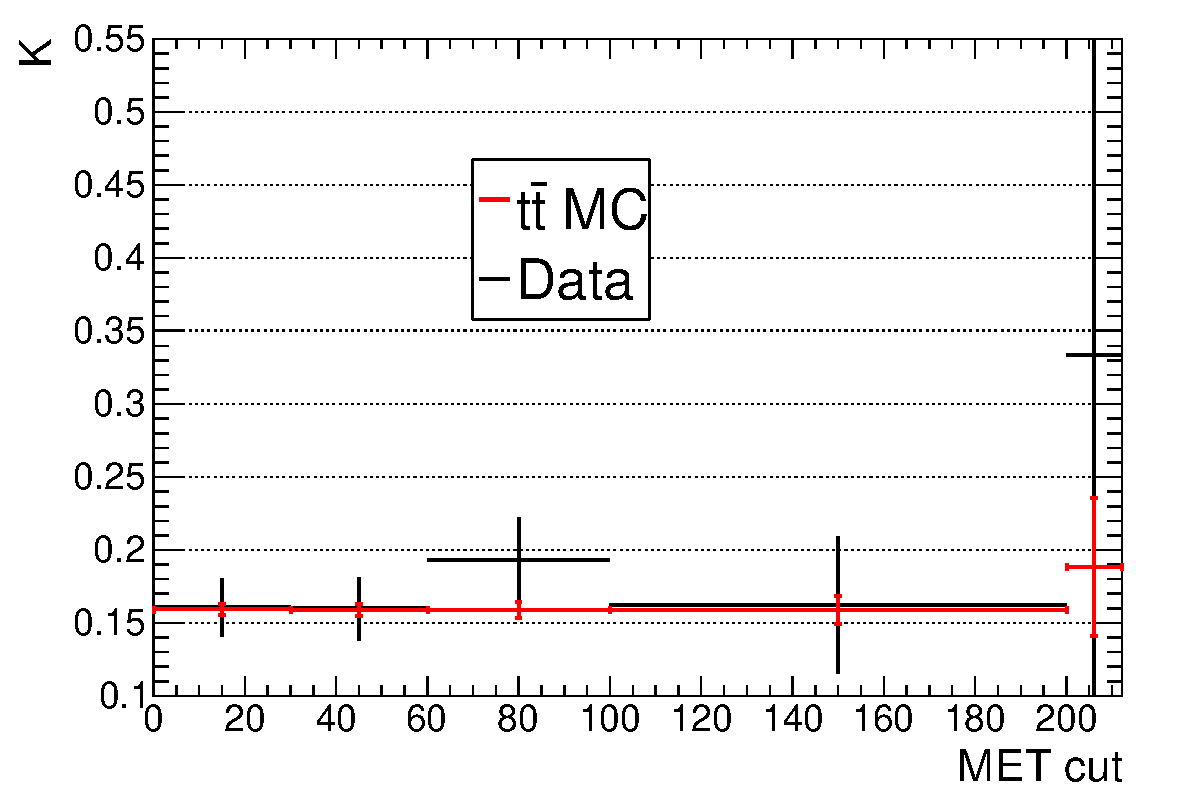
\includegraphics[width=0.48\linewidth]{plots/kvmet_data_ttbm.pdf}
%	\includegraphics[width=0.48\linewidth]{plots/kvmet_ratio.pdf}
%	\caption{
%	  \label{fig:kvmet}\protect 
%	  The left plot shows
%	  K as a function of \MET\ in MC (red) and data (black). 
%	  The bin low edge corresponds to the \MET\ cut, and the 
%	  bins are inclusive.
%	  The MC used is a sum of all SM MC used in the yield table of
%	  section \ref{sec:yields}.
%	  The right plot is the ratio of K in data to MC.
%	  The ratio is fit to a line whose slope is consistent with zero
%	  (the fit parameters are 
%	  0.9 $\pm$  0.4 for the intercept and
%      0.001 $\pm$ 0.005 for the slope).
%	}
%  \end{center}
%\end{figure}
%
%
%
%\begin{table}[htb]
%\begin{center}
%\caption{\label{fig:kvmettable} The values of K used in the OF background prediction. 
%The uncertainties shown are the total relative systematic used for the OF prediction,
%which is the systematic uncertainty from K added in quadrature with
%a 7\% uncertainty from the electron to muon efficieny ratio as assessed in the
%inclusive analysis.
%}
%\begin{tabular}{lcc}
%\hline
%\MET\ Cut    &    K        &  Relative Systematic \\
%\hline
%%the met zero row is used only for normalization of the money plot.
%%0    &  0.1   &        \\  
%30   &  0.12  &  20\%  \\  
%60   &  0.13  &  20\%  \\  
%80   &  0.12  &  20\%  \\  
%100  &  0.12  &  20\%  \\  
%150  &  0.09  &  25\%  \\  
%200  &  0.06  &  60\%  \\  
%\hline
%\end{tabular}
%\end{center}
%\end{table}

\subsection{Uncertainty from the isolated track veto}
This is the uncertainty associated with how well the isolated track
veto performance is modeled by the Monte Carlo.  This uncertainty
only applies to the fraction of dilepton BG events that have 
a second e/$\mu$ or a one prong $\tau \to h$, with 
$P_T > 10$ GeV in $|\eta| < 2.4$.  This fraction is about 1/3, see 
Table~\ref{tab:trueisotrk}.
The uncertainty for these events
is 6\% and is obtained from tag-and-probe studies, see Section~\ref{sec:trkveto}.

\begin{table}[!h]
\begin{center}
{\footnotesize
\begin{tabular}{l||c|c|c|c|c|c|c}
\hline
Sample              & SRA & SRB & SRC & SRD & SRE & SRF & SRG \\
\hline
\hline
$\mu$ Frac. \ttdl\ with true iso. trk. 	 & $0.32 \pm 0.03$ & $0.30 \pm 0.03$ & $0.32 \pm 0.06$ & $0.34 \pm 0.10$ & $0.35 \pm 0.16$ & $0.40 \pm 0.24$ & $0.50 \pm 0.32$  \\
\hline
\hline
e Frac. \ttdl\ with true iso. trk. 	 & $0.32 \pm 0.03$ & $0.31 \pm 0.04$ & $0.33 \pm 0.06$ & $0.38 \pm 0.11$ & $0.38 \pm 0.19$ & $0.60 \pm 0.31$ & $0.61 \pm 0.45$  \\
\hline
\end{tabular}}
\caption{ Fraction of \ttdl\ events with a true isolated track.
\label{tab:trueisotrk}}
\end{center}
\end{table}

\subsubsection{Isolated Track Veto: Tag and Probe Studies}
\label{sec:trkveto}


In this section we compare the performance of the isolated track veto in data and MC using tag-and-probe studies
with samples of Z$\to$ee and Z$\to\mu\mu$. The purpose of these studies is to demonstrate that the efficiency
to satisfy the isolated track veto requirements is well-reproduced in the MC, since if this were not the case 
we would need to apply a data-to-MC scale factor in order to correctly
predict the \ttll\ background. 

This study
addresses possible data vs. MC discrepancies for the {\bf efficiency} to identify (and reject) events with a 
second {\bf genuine} lepton (e, $\mu$, or $\tau\to$1-prong). It does not address possible data vs. MC discrepancies
in the fake rate for rejecting events without a second genuine lepton; this is handled separately in the top normalization
procedure by scaling the \ttlj\ contribution to match the data in the \mt\ peak after applying the isolated track veto. 

Furthermore, we test the data and MC
isolated track veto efficiencies for electrons and muons since we are using a Z tag-and-probe technique, but we do not
directly test the performance for hadronic tracks from $\tau$ decays. The performance for hadronic $\tau$ decay products
may differ from that of electrons and muons for two reasons. First, the $\tau$ may decay to a hadronic track plus one
or two $\pi^0$'s, which may decay to $\gamma\gamma$ followed by a photon conversion. As shown in Figure~\ref{fig:absiso},
the isolation distribution for charged tracks from $\tau$ decays that are not produced in association with $\pi^0$s are 
consistent with that from $\E$s and $\M$s. Since events from single prong $\tau$ decays produced in association with 
$\pi^0$s comprise a small fraction of the total sample, and since the kinematics of $\tau$, $\pi^0$ and $\gamma\to e^+e^-$
decays are well-understood, we currently demonstrate that the isolation is well-reproduced for electrons and muons only.
Second, hadronic tracks may undergo nuclear interactions and hence their tracks may not be reconstructed.
As discussed above, independent studies show that the MC reproduces the hadronic tracking efficiency within 4\%,
leading to a total background uncertainty of less than 0.5\% (after taking into account the fraction of the total background
due to hadronic $\tau$ decays with \pt\ $>$ 10 GeV tracks), and we hence regard this effect as negligible.

The tag-and-probe studies are performed in the full data sample, and compared with the DYJets madgraph sample.
All events must contain a tag-probe pair (details below) with opposite-sign and satisfying the Z mass requirement 76--106 GeV.
We compare the distributions of absolute track isolation for probe electrons/muons in data vs. MC. The contributions to
this isolation sum are from ambient energy in the event from underlying event, pile-up and jet activitiy, and hence do
not depend on the \pt\ of the probe lepton. We therefore restrict the probe \pt\ to be $>$ 30 GeV in order to suppress
fake backgrounds with steeply-falling \pt\ spectra. To suppress non-Z backgrounds (in particular \ttbar) we require 
\met\ $<$ 30 GeV and 0 b-tagged events. 
The specific criteria for tags and probes for electrons and muons are:

%We study the isolated track veto efficiency in bins of \njets.
%We are interested in events with at least 4 jets to emulate the hadronic activity in our signal sample. However since
%there are limited statistics for Z + $\geq$4 jet events, we study the isolated track performance in events with


\begin{itemize}
  \item{Electrons}

    \begin{itemize}
    \item{Tag criteria}

      \begin{itemize}
      \item Electron passes full analysis ID/iso selection 
      \item \pt\ $>$ 30 GeV, $|\eta|<2.1$ 
      \item Matched to the single electron trigger \verb=HLT_Ele27_WP80_v*=
      \end{itemize}

    \item{Probe criteria}
      \begin{itemize}
      \item Electron passes full analysis ID selection
      \item \pt\ $>$ 30 GeV
      \end{itemize}
      \end{itemize}
  \item{Muons}
    \begin{itemize}
    \item{Tag criteria}
      \begin{itemize}
      \item Muon passes full analysis ID/iso selection
      \item \pt\ $>$ 30 GeV, $|\eta|<2.1$
      \item Matched to 1 of the 2 single muon triggers
        \begin{itemize}
        \item \verb=HLT_IsoMu30_v*=
        \item \verb=HLT_IsoMu30_eta2p1_v*=
        \end{itemize}
      \end{itemize}
    \item{Probe criteria}
      \begin{itemize}
      \item Muon passes full analysis ID selection
      \item \pt\ $>$ 30 GeV
      \end{itemize}
    \end{itemize}
\end{itemize}

The absolute track isolation distributions for passing probes are displayed in Fig.~\ref{fig:tnp}. In general we observe
good agreement between data and MC. To be more quantitative, we compare the data vs. MC efficiencies to satisfy
absolute track isolation requirements varying from $>$ 1 GeV to $>$ 5 GeV, as summarized in Table~\ref{tab:isotrk}.
In the $\geq 0$ and $\geq 1$ jet bins where the efficiencies can be tested with statistical precision, the data and MC
efficiencies agree within 6\%, and we apply this as a systematic uncertainty on the isolated track veto efficiency.
For the higher jet multiplicity bins the statistical precision decreases, but we do not observe any evidence for
a data vs. MC discrepancy in the isolated track veto efficiency.


%This is because our analysis requirement is relative track isolation $<$ 0.1, and m
%This requirement is chosen because most of the tracks rejected by the isolated
%track veto have a \pt\ near the 10 GeV threshold, and our analysis requirement is relative track isolation $<$ 1 GeV.

\begin{figure}[hbt]
  \begin{center}
  	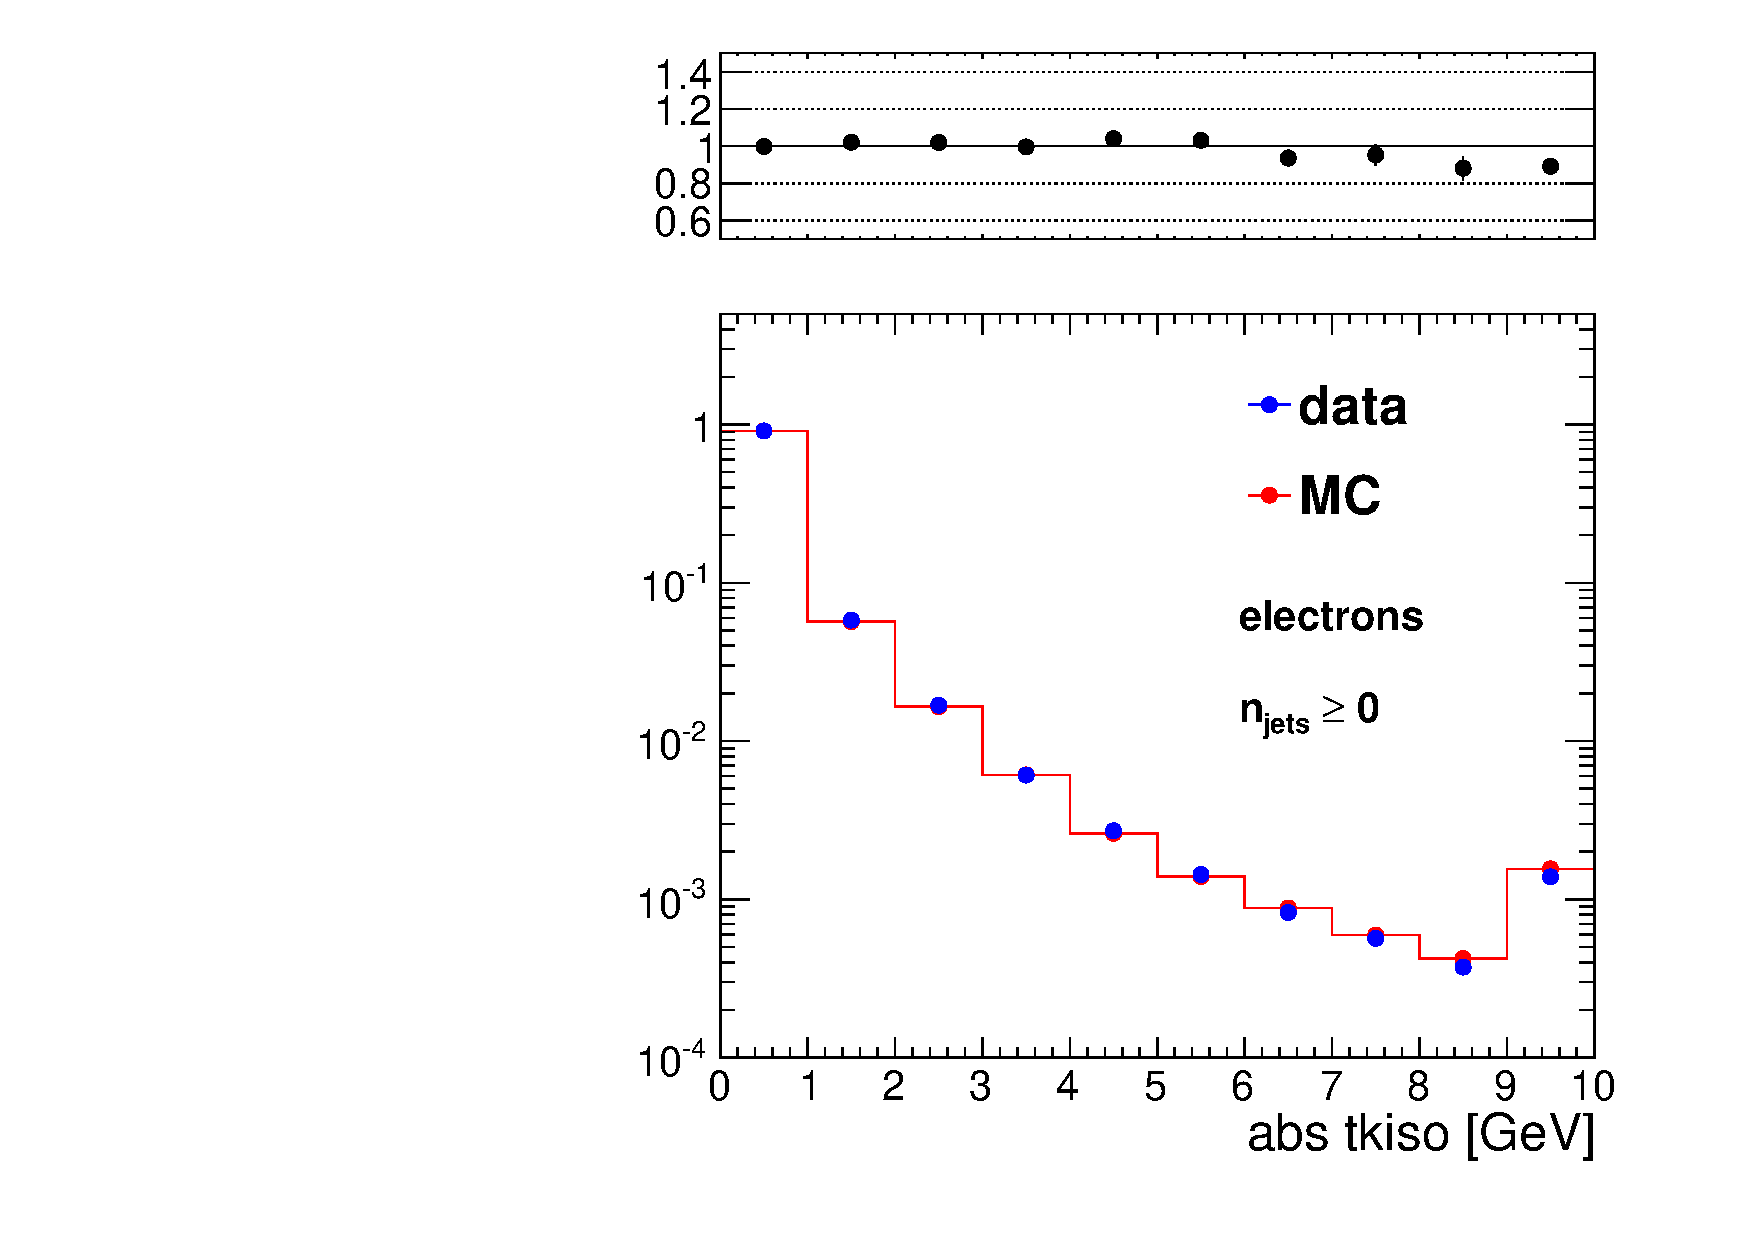
\includegraphics[width=0.3\linewidth]{plots/el_tkiso_0j.pdf}%
	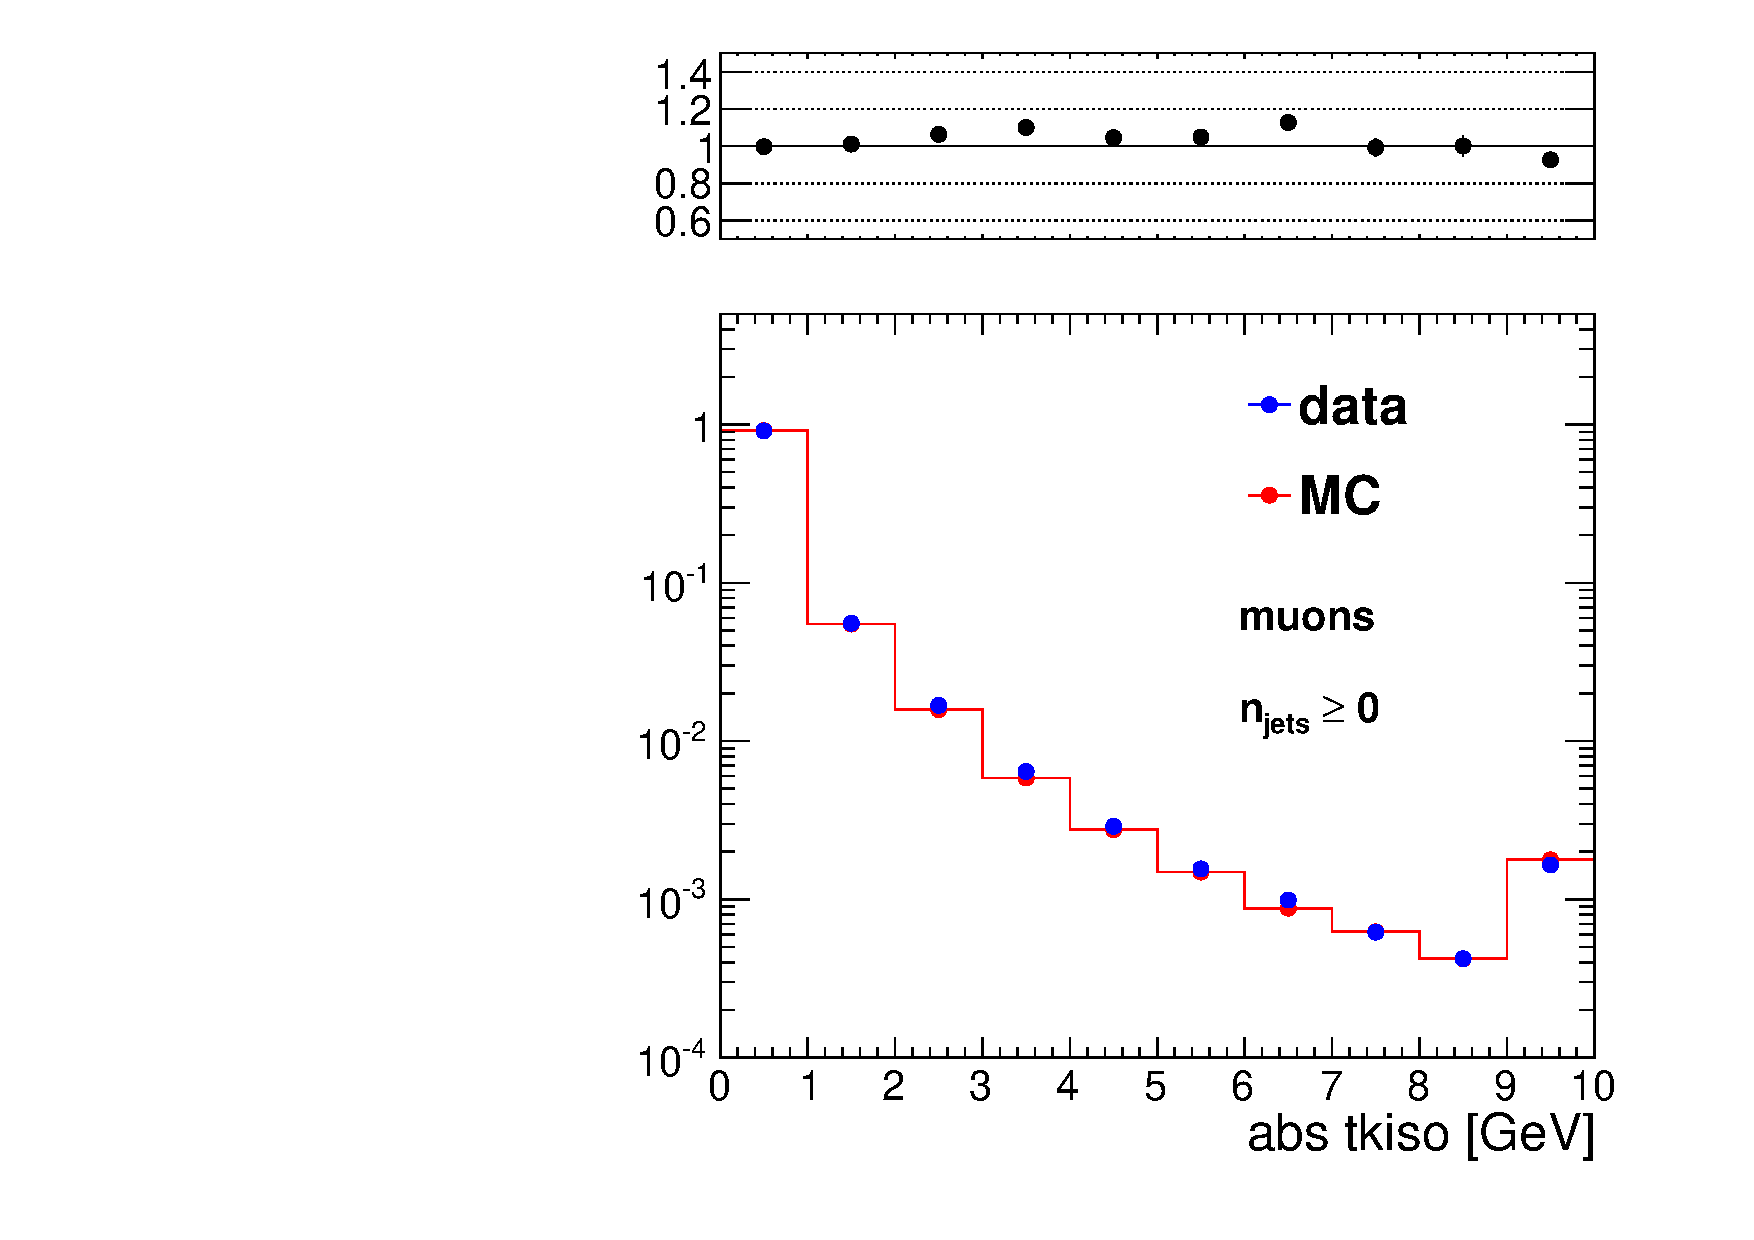
\includegraphics[width=0.3\linewidth]{plots/mu_tkiso_0j.pdf}
	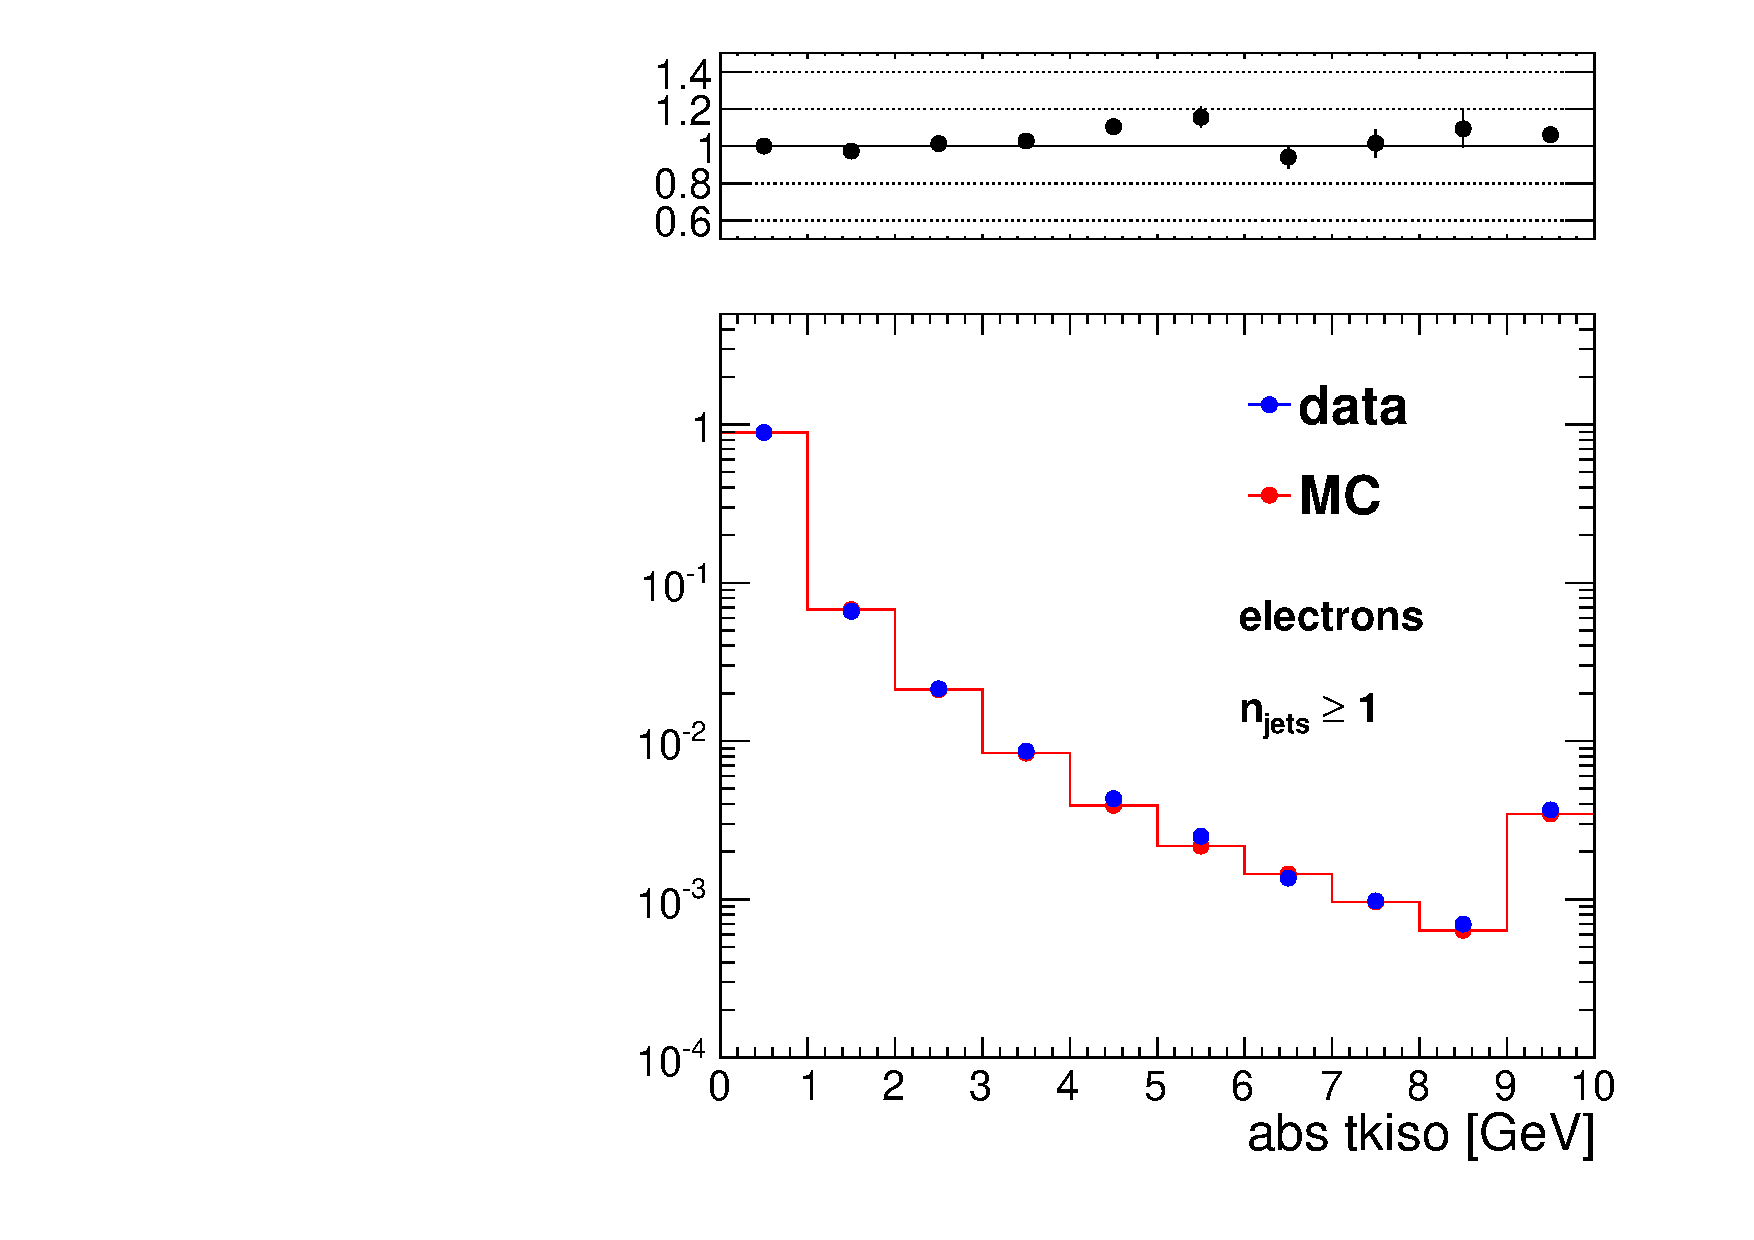
\includegraphics[width=0.3\linewidth]{plots/el_tkiso_1j.pdf}%
	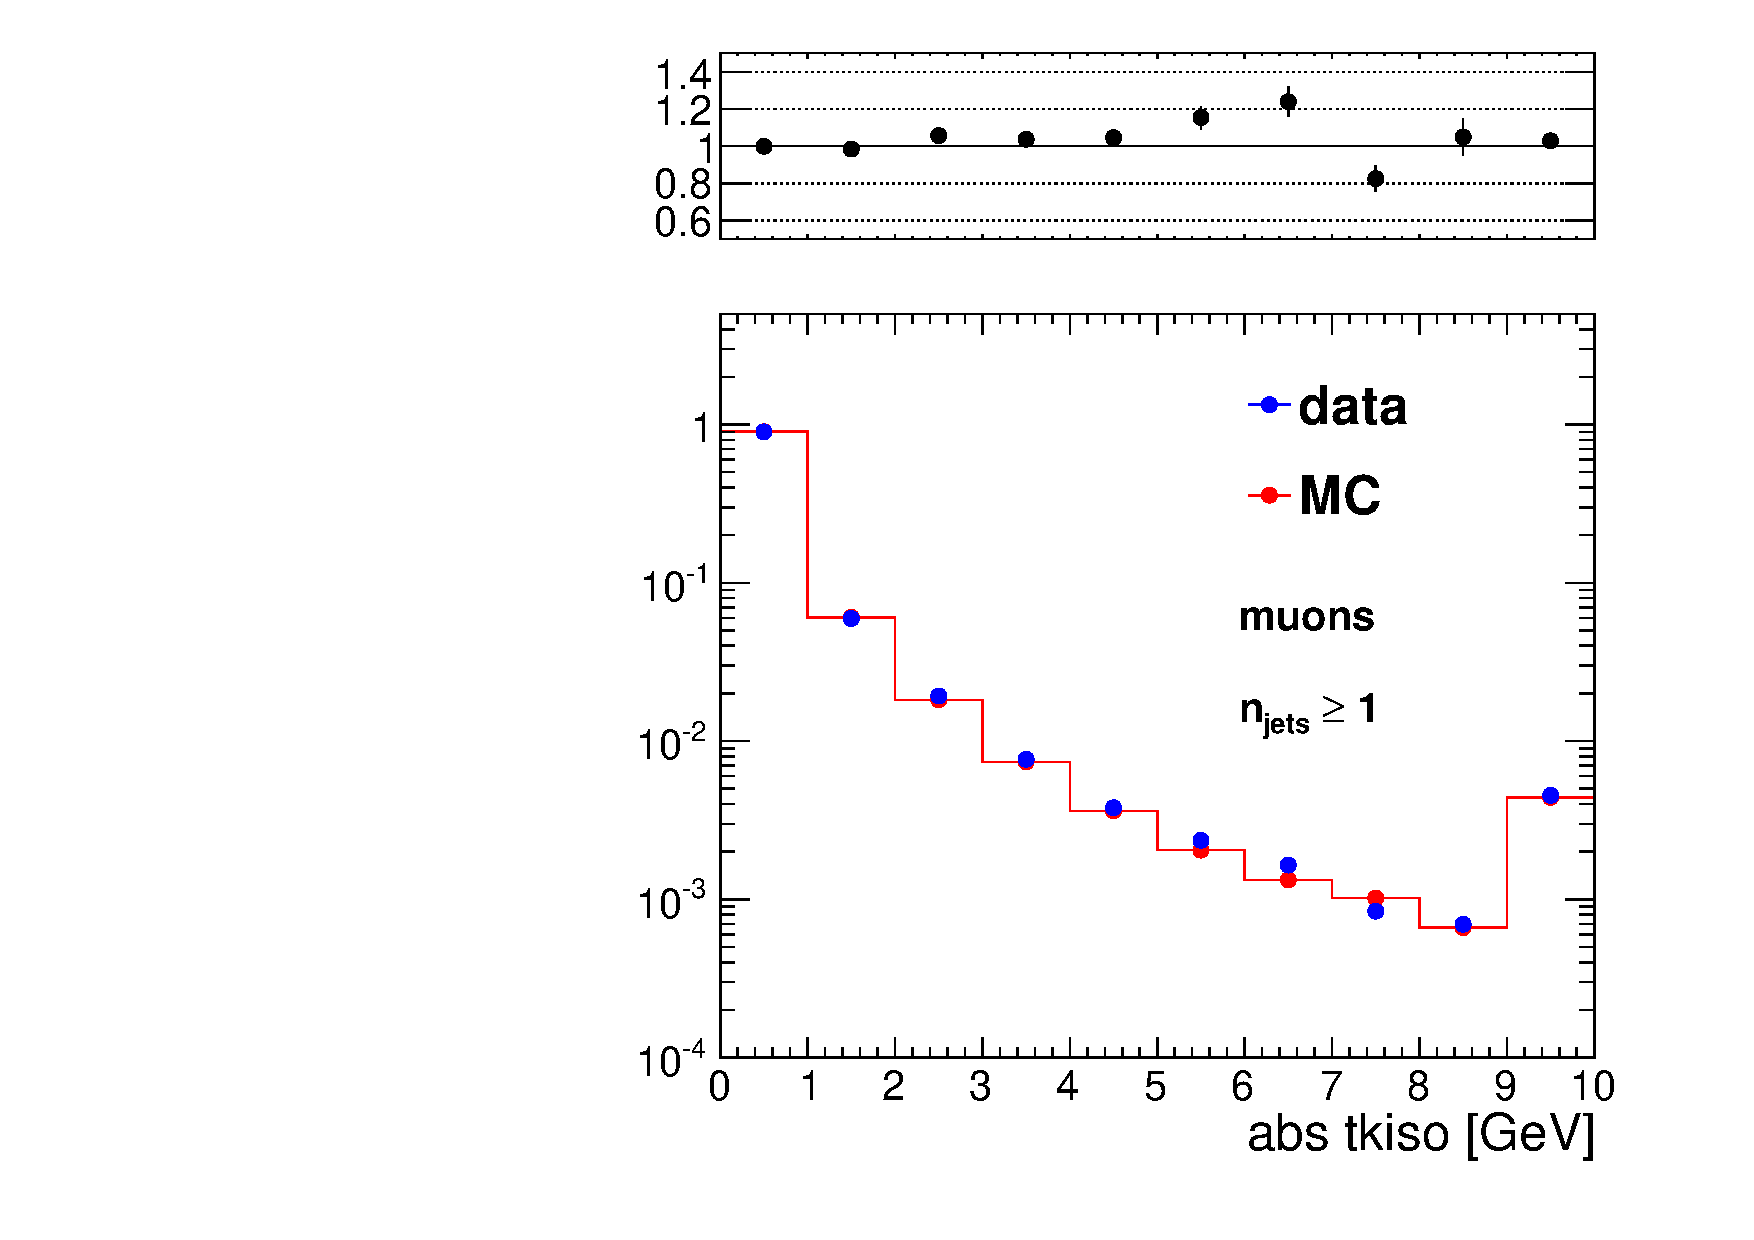
\includegraphics[width=0.3\linewidth]{plots/mu_tkiso_1j.pdf}
	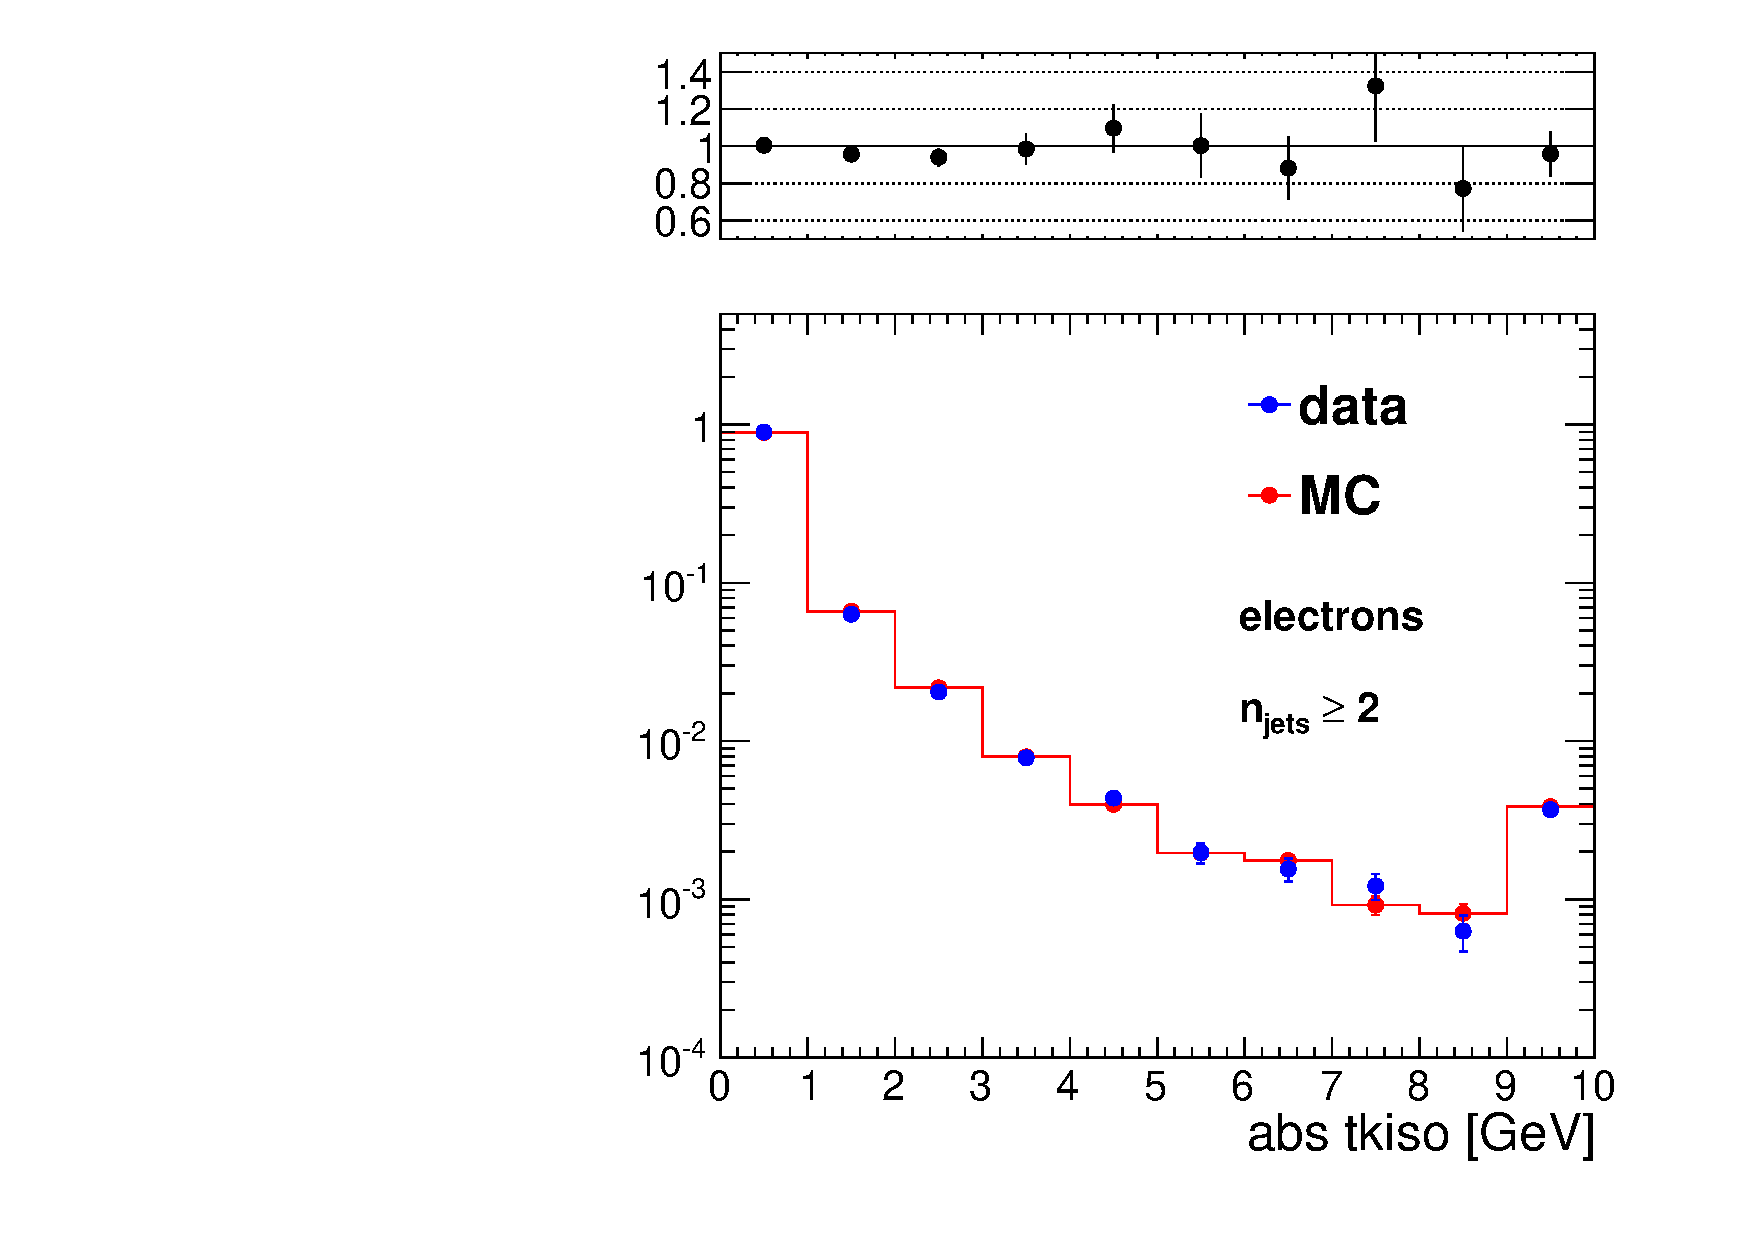
\includegraphics[width=0.3\linewidth]{plots/el_tkiso_2j.pdf}%
	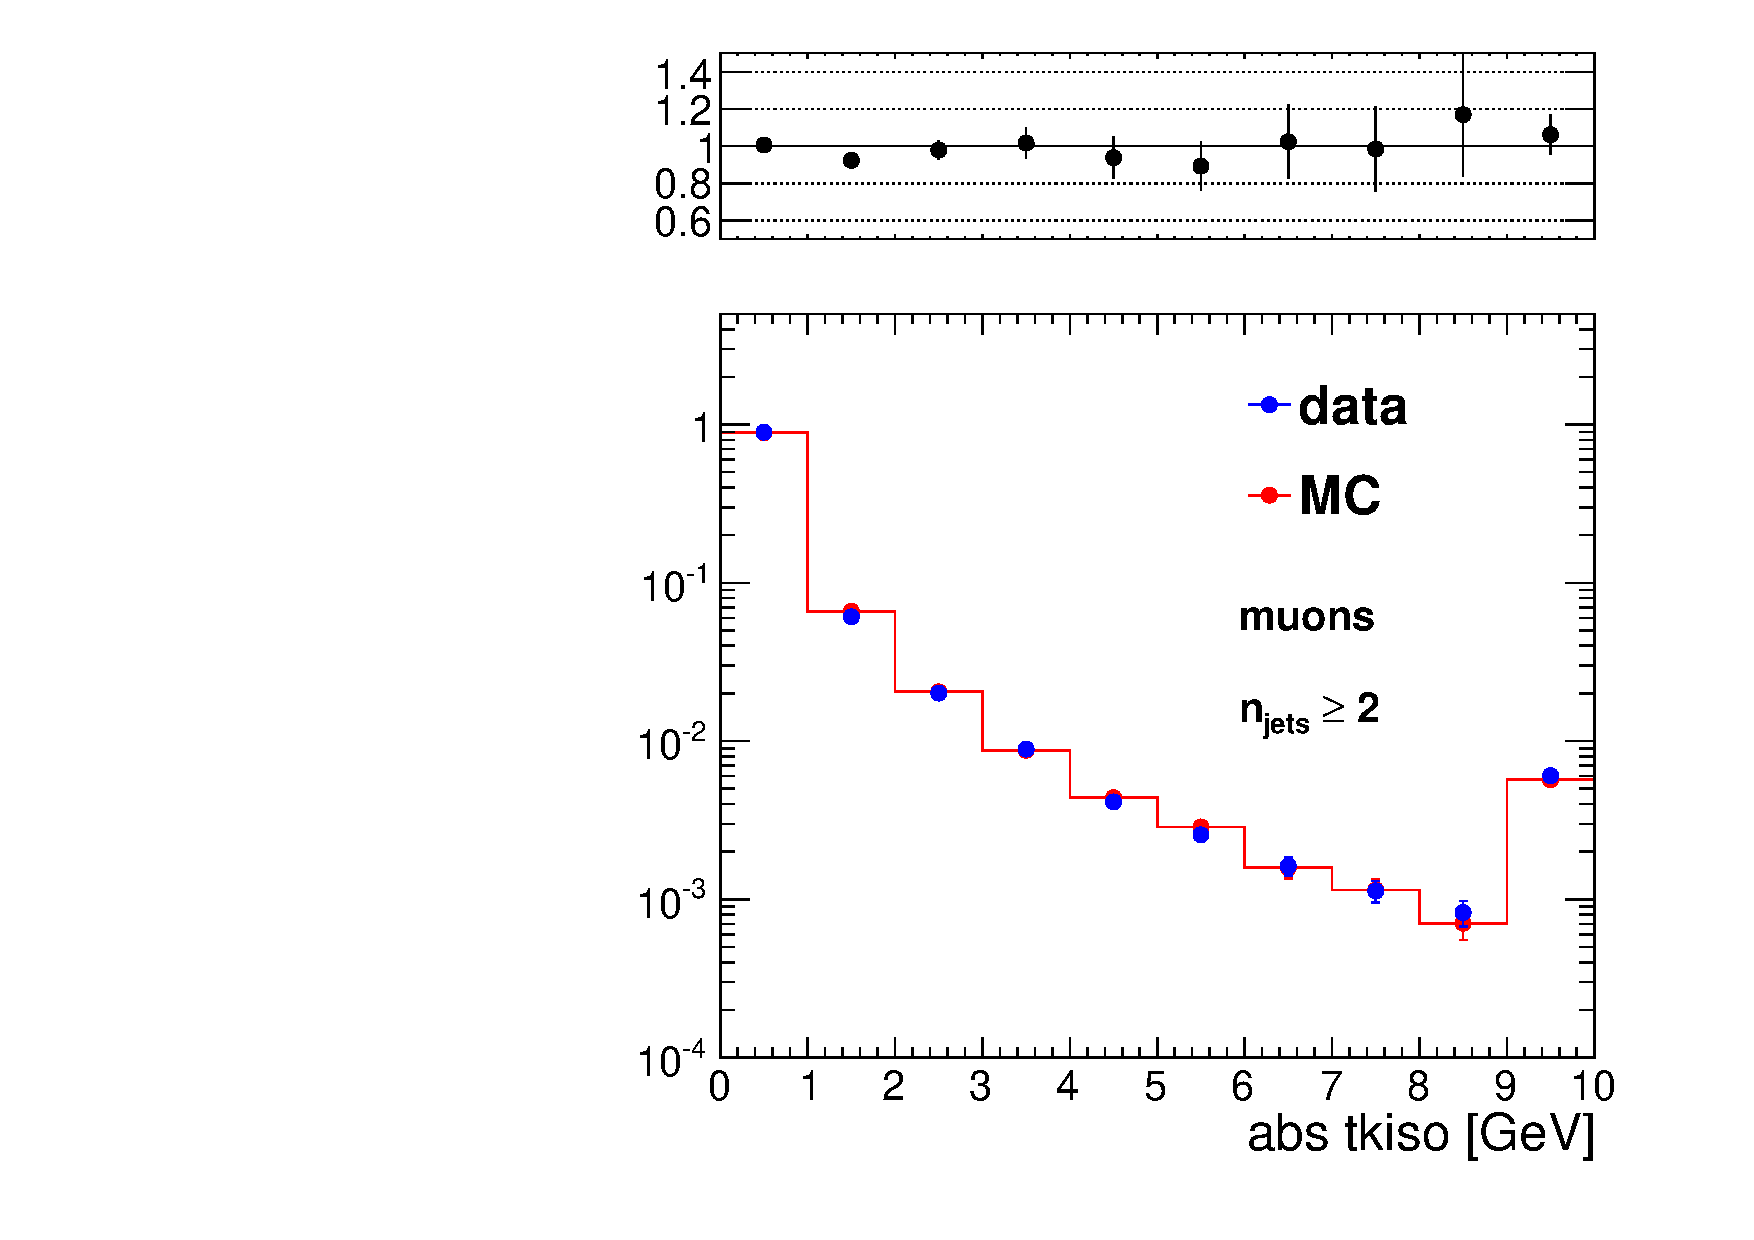
\includegraphics[width=0.3\linewidth]{plots/mu_tkiso_2j.pdf}
	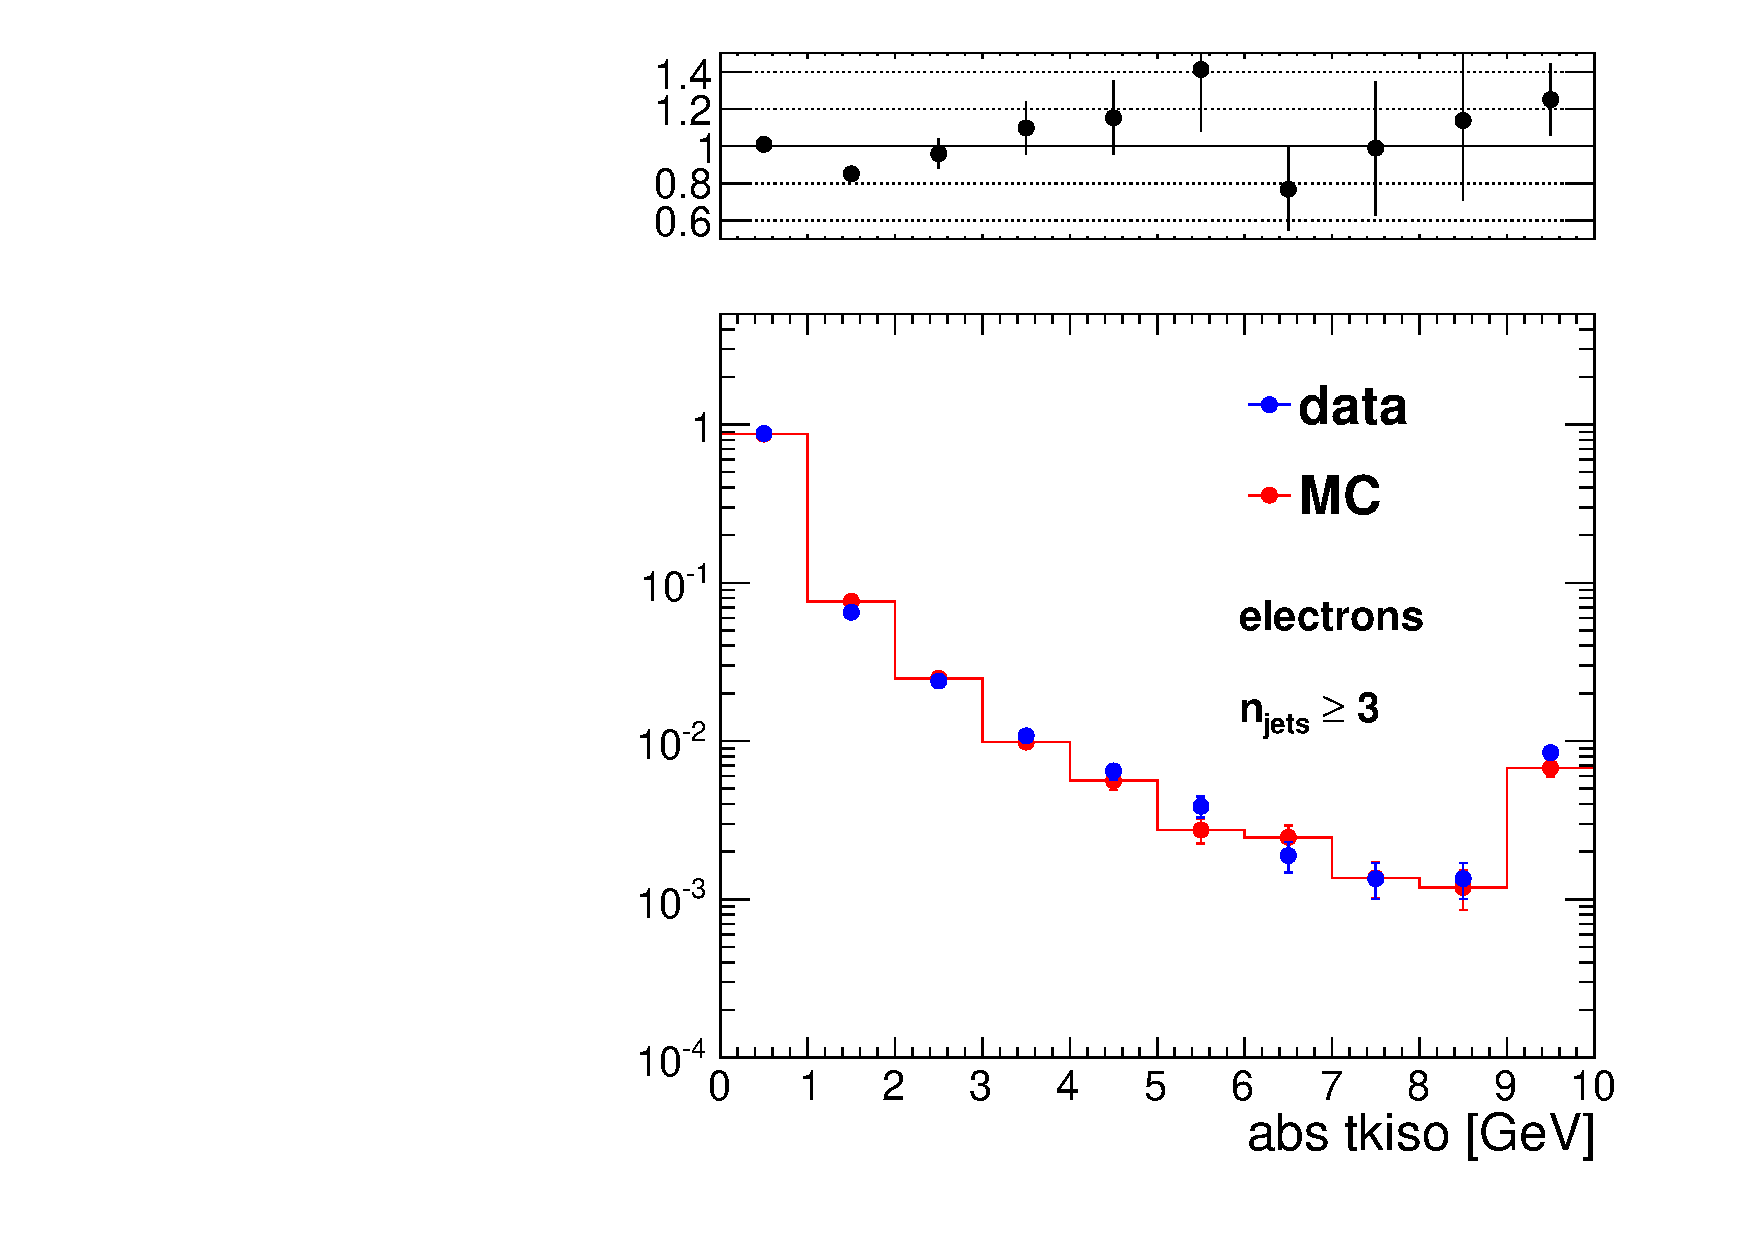
\includegraphics[width=0.3\linewidth]{plots/el_tkiso_3j.pdf}%
	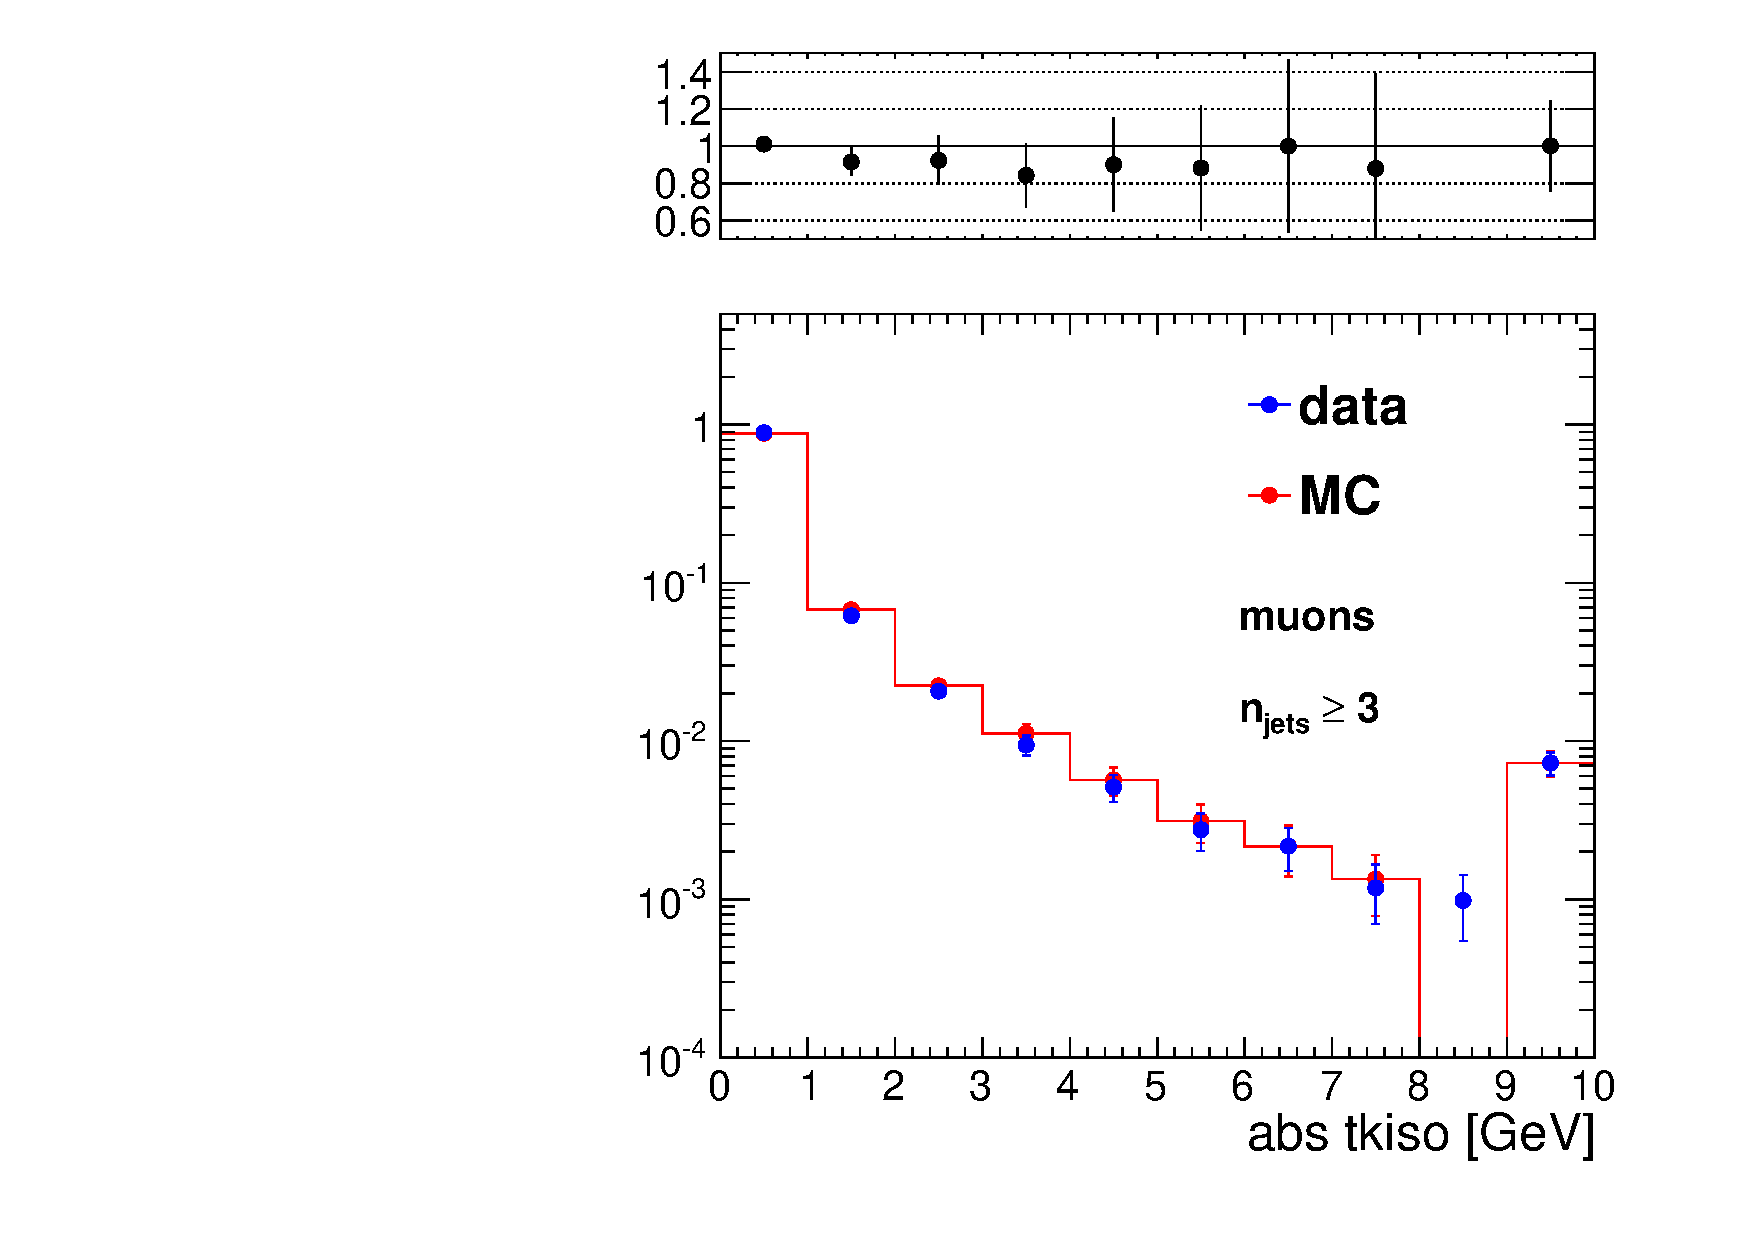
\includegraphics[width=0.3\linewidth]{plots/mu_tkiso_3j.pdf}
	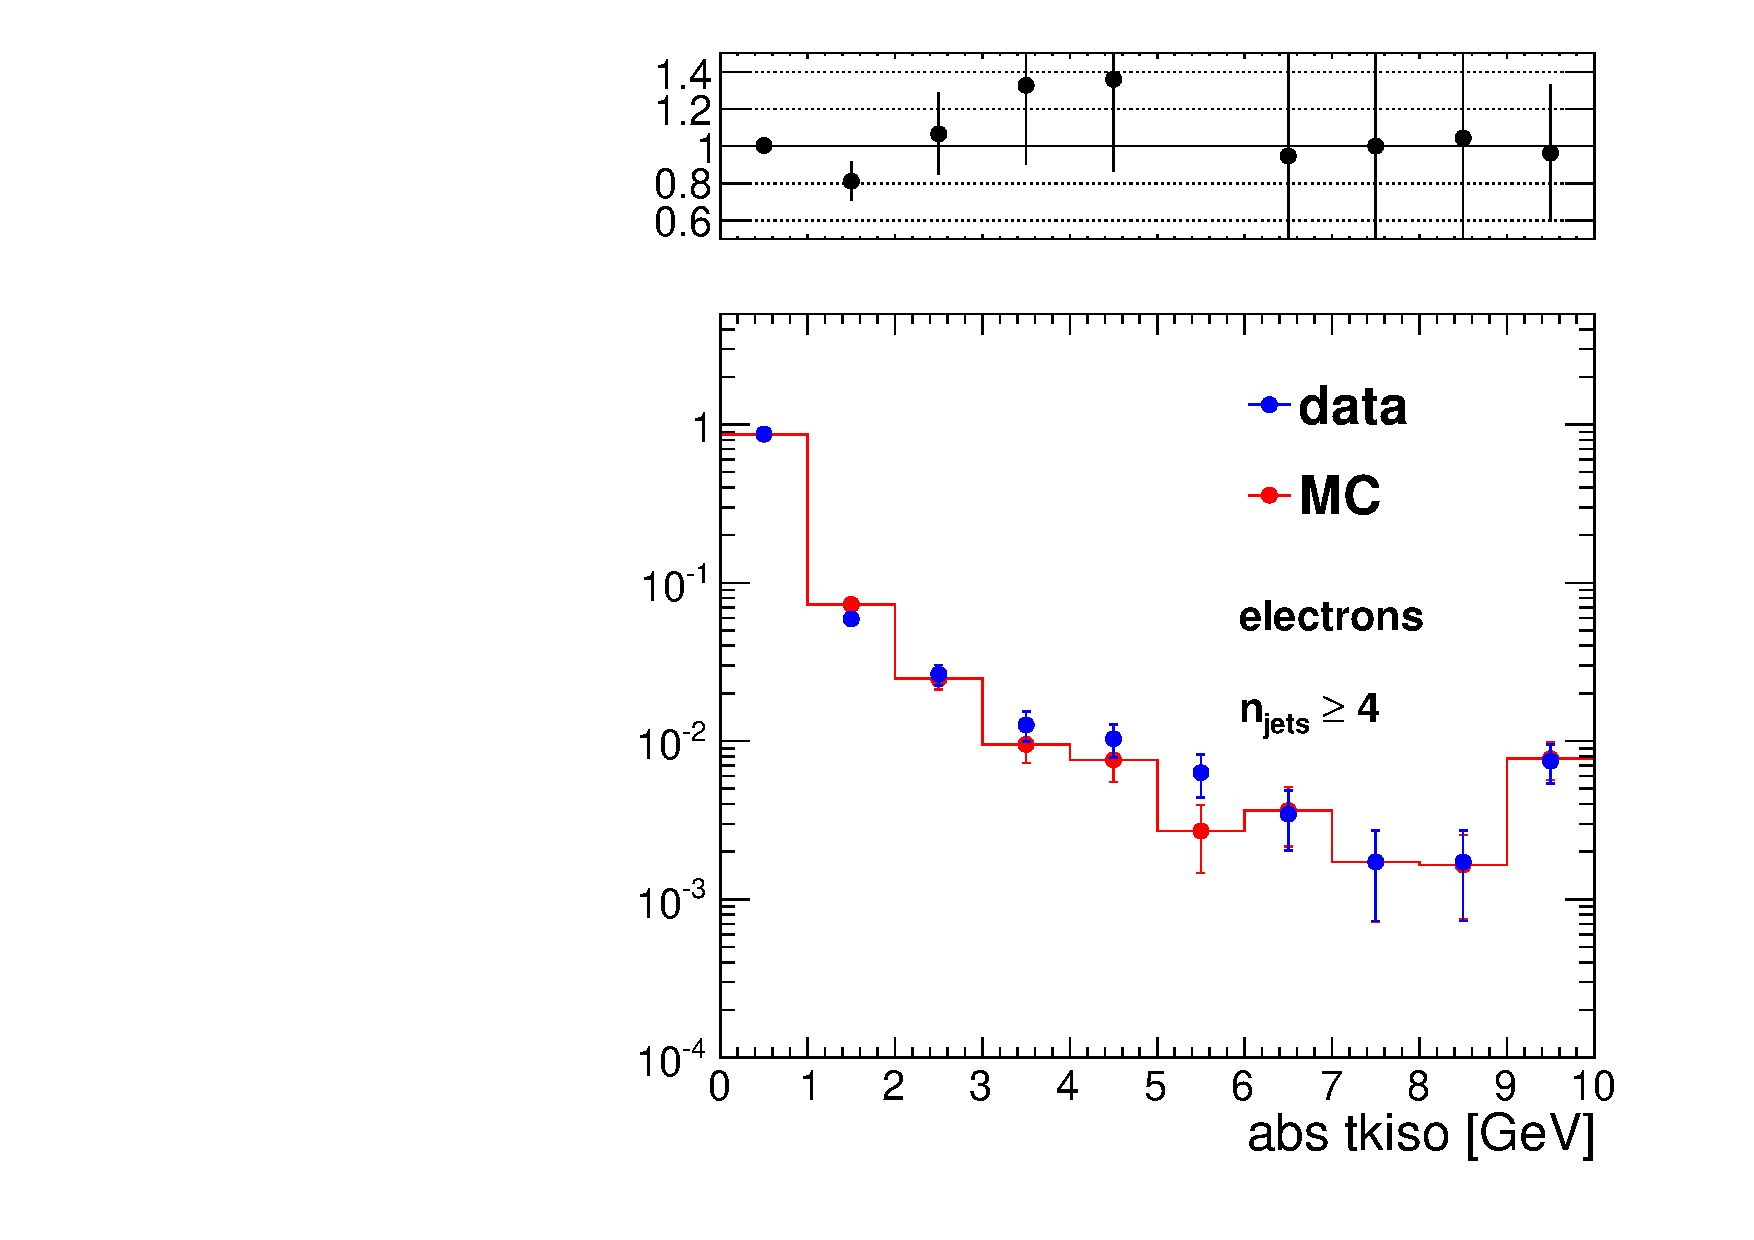
\includegraphics[width=0.3\linewidth]{plots/el_tkiso_4j.pdf}%
	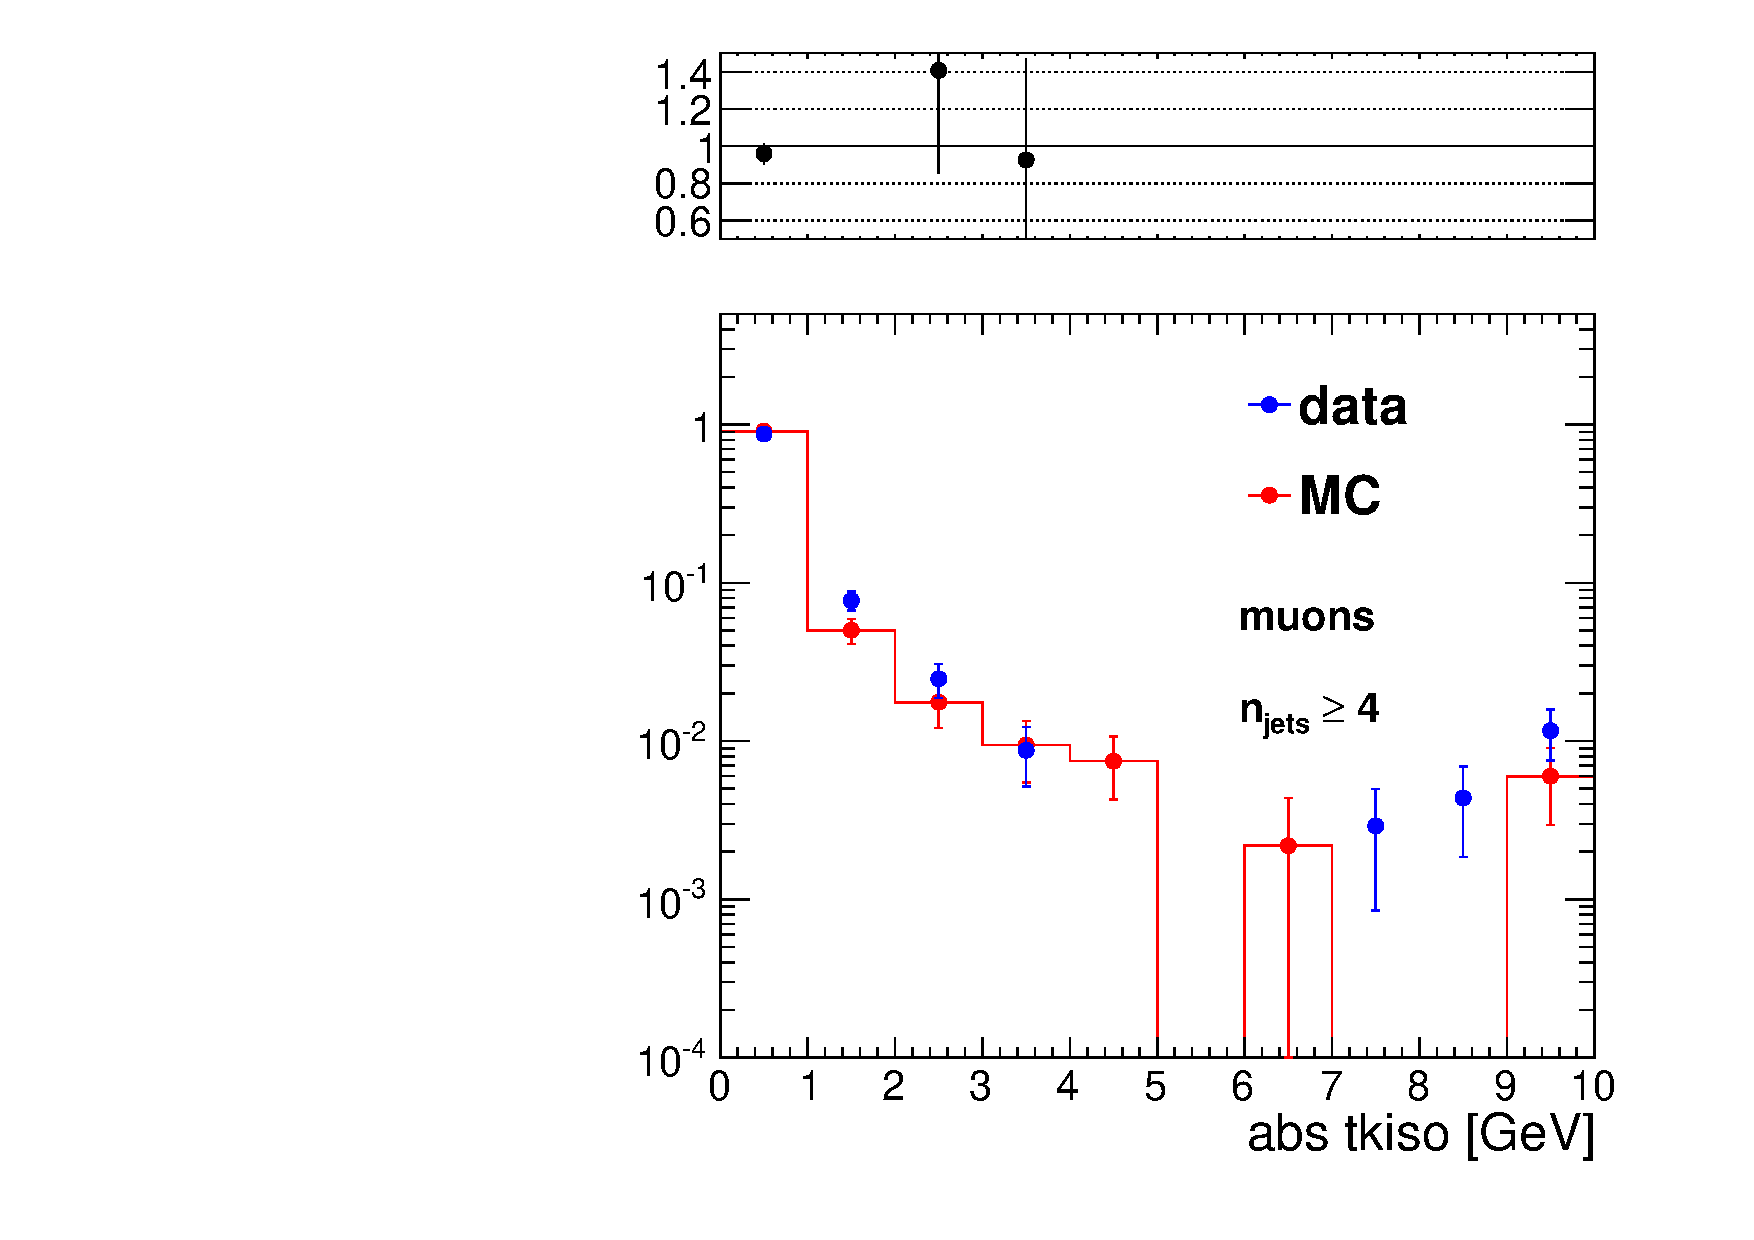
\includegraphics[width=0.3\linewidth]{plots/mu_tkiso_4j.pdf}
	\caption{
	  \label{fig:tnp} Comparison of the absolute track isolation in data vs. MC for electrons (left) and muons (right)
for events with the \njets\ requirement varied from \njets\ $\geq$ 0 to \njets\ $\geq$ 4. 
}  
      \end{center}
\end{figure}

\clearpage

\begin{table}[!ht]
\begin{center}
\begin{tabular}{l|c|c|c|c|c}

%Electrons:
%Selection            : ((((((((((abs(tagAndProbeMass-91)<15)&&(qProbe*qTag<0))&&((eventSelection&1)==1))&&(abs(tag->eta())<2.1))&&(tag->pt()>30.0))&&(HLT_Ele27_WP80_tag > 0))&&(met<30))&&(nbl==0))&&((leptonSelection&8)==8))&&(probe->pt()>30))&&(drprobe<0.05)
%Total MC yields 	: 2497277
%Total DATA yields 	: 2649453
%Muons:
%Selection            : ((((((((((abs(tagAndProbeMass-91)<15)&&(qProbe*qTag<0))&&((eventSelection&2)==2))&&(abs(tag->eta())<2.1))&&(tag->pt()>30.0))&&(HLT_IsoMu24_tag > 0))&&(met<30))&&(nbl==0))&&((leptonSelection&65536)==65536))&&(probe->pt()>30))&&(drprobe<0.05)
%Total MC yields 	: 3749863
%Total DATA yields 	: 4210022
%Info in <TCanvas::MakeDefCanvas>:  created default TCanvas with name c1
%Info in <TCanvas::Print>: pdf file plots/nvtx.pdf has been created

\hline
\hline
e + $\geq$0 jets   &           $>$ 1 GeV   &           $>$ 2 GeV   &           $>$ 3 GeV   &           $>$ 4 GeV   &           $>$ 5 GeV  \\
\hline
      data   &  0.098 $\pm$ 0.0002   &  0.036 $\pm$ 0.0001   &  0.016 $\pm$ 0.0001   &  0.009 $\pm$ 0.0001   &  0.006 $\pm$ 0.0000  \\
        mc   &  0.097 $\pm$ 0.0002   &  0.034 $\pm$ 0.0001   &  0.016 $\pm$ 0.0001   &  0.009 $\pm$ 0.0001   &  0.005 $\pm$ 0.0000  \\
   data/mc   &     1.00 $\pm$ 0.00   &     1.04 $\pm$ 0.00   &     1.04 $\pm$ 0.01   &     1.03 $\pm$ 0.01   &     1.02 $\pm$ 0.01  \\

\hline
\hline
$\mu$ + $\geq$0 jets   &           $>$ 1 GeV   &           $>$ 2 GeV   &           $>$ 3 GeV   &           $>$ 4 GeV   &           $>$ 5 GeV  \\
\hline
      data   &  0.094 $\pm$ 0.0001   &  0.034 $\pm$ 0.0001   &  0.016 $\pm$ 0.0001   &  0.009 $\pm$ 0.0000   &  0.006 $\pm$ 0.0000  \\
        mc   &  0.093 $\pm$ 0.0001   &  0.033 $\pm$ 0.0001   &  0.015 $\pm$ 0.0001   &  0.009 $\pm$ 0.0000   &  0.006 $\pm$ 0.0000  \\
   data/mc   &     1.01 $\pm$ 0.00   &     1.03 $\pm$ 0.00   &     1.03 $\pm$ 0.01   &     1.03 $\pm$ 0.01   &     1.02 $\pm$ 0.01  \\

\hline
\hline
e + $\geq$1 jets   &           $>$ 1 GeV   &           $>$ 2 GeV   &           $>$ 3 GeV   &           $>$ 4 GeV   &           $>$ 5 GeV  \\
\hline
      data   &  0.110 $\pm$ 0.0005   &  0.044 $\pm$ 0.0003   &  0.022 $\pm$ 0.0002   &  0.014 $\pm$ 0.0002   &  0.009 $\pm$ 0.0002  \\
        mc   &  0.110 $\pm$ 0.0005   &  0.042 $\pm$ 0.0003   &  0.021 $\pm$ 0.0002   &  0.013 $\pm$ 0.0002   &  0.009 $\pm$ 0.0001  \\
   data/mc   &     1.00 $\pm$ 0.01   &     1.04 $\pm$ 0.01   &     1.06 $\pm$ 0.02   &     1.08 $\pm$ 0.02   &     1.06 $\pm$ 0.03  \\

\hline
\hline
$\mu$ + $\geq$1 jets   &           $>$ 1 GeV   &           $>$ 2 GeV   &           $>$ 3 GeV   &           $>$ 4 GeV   &           $>$ 5 GeV  \\
\hline
      data   &  0.106 $\pm$ 0.0004   &  0.043 $\pm$ 0.0003   &  0.023 $\pm$ 0.0002   &  0.014 $\pm$ 0.0002   &  0.010 $\pm$ 0.0001  \\
        mc   &  0.106 $\pm$ 0.0004   &  0.042 $\pm$ 0.0003   &  0.021 $\pm$ 0.0002   &  0.013 $\pm$ 0.0002   &  0.009 $\pm$ 0.0001  \\
   data/mc   &     1.00 $\pm$ 0.01   &     1.04 $\pm$ 0.01   &     1.06 $\pm$ 0.01   &     1.08 $\pm$ 0.02   &     1.07 $\pm$ 0.02  \\

\hline
\hline
e + $\geq$2 jets   &           $>$ 1 GeV   &           $>$ 2 GeV   &           $>$ 3 GeV   &           $>$ 4 GeV   &           $>$ 5 GeV  \\
\hline
      data   &  0.117 $\pm$ 0.0012   &  0.050 $\pm$ 0.0008   &  0.026 $\pm$ 0.0006   &  0.017 $\pm$ 0.0005   &  0.012 $\pm$ 0.0004  \\
        mc   &  0.120 $\pm$ 0.0012   &  0.048 $\pm$ 0.0008   &  0.025 $\pm$ 0.0006   &  0.016 $\pm$ 0.0005   &  0.011 $\pm$ 0.0004  \\
   data/mc   &     0.97 $\pm$ 0.01   &     1.05 $\pm$ 0.02   &     1.05 $\pm$ 0.03   &     1.07 $\pm$ 0.04   &     1.07 $\pm$ 0.05  \\

\hline
\hline
$\mu$ + $\geq$2 jets   &           $>$ 1 GeV   &           $>$ 2 GeV   &           $>$ 3 GeV   &           $>$ 4 GeV   &           $>$ 5 GeV  \\
\hline
      data   &  0.111 $\pm$ 0.0010   &  0.048 $\pm$ 0.0007   &  0.026 $\pm$ 0.0005   &  0.018 $\pm$ 0.0004   &  0.013 $\pm$ 0.0004  \\
        mc   &  0.115 $\pm$ 0.0010   &  0.048 $\pm$ 0.0006   &  0.025 $\pm$ 0.0005   &  0.016 $\pm$ 0.0004   &  0.012 $\pm$ 0.0003  \\
   data/mc   &     0.97 $\pm$ 0.01   &     1.01 $\pm$ 0.02   &     1.04 $\pm$ 0.03   &     1.09 $\pm$ 0.04   &     1.09 $\pm$ 0.04  \\

\hline
\hline
e + $\geq$3 jets   &           $>$ 1 GeV   &           $>$ 2 GeV   &           $>$ 3 GeV   &           $>$ 4 GeV   &           $>$ 5 GeV  \\
\hline
      data   &  0.123 $\pm$ 0.0031   &  0.058 $\pm$ 0.0022   &  0.034 $\pm$ 0.0017   &  0.023 $\pm$ 0.0014   &  0.017 $\pm$ 0.0012  \\
        mc   &  0.131 $\pm$ 0.0030   &  0.055 $\pm$ 0.0020   &  0.030 $\pm$ 0.0015   &  0.020 $\pm$ 0.0013   &  0.015 $\pm$ 0.0011  \\
   data/mc   &     0.94 $\pm$ 0.03   &     1.06 $\pm$ 0.06   &     1.14 $\pm$ 0.08   &     1.16 $\pm$ 0.10   &     1.17 $\pm$ 0.12  \\

\hline
\hline
$\mu$ + $\geq$3 jets   &           $>$ 1 GeV   &           $>$ 2 GeV   &           $>$ 3 GeV   &           $>$ 4 GeV   &           $>$ 5 GeV  \\
\hline
      data   &  0.121 $\pm$ 0.0025   &  0.055 $\pm$ 0.0018   &  0.033 $\pm$ 0.0014   &  0.022 $\pm$ 0.0011   &  0.017 $\pm$ 0.0010  \\
        mc   &  0.120 $\pm$ 0.0024   &  0.052 $\pm$ 0.0016   &  0.029 $\pm$ 0.0012   &  0.019 $\pm$ 0.0010   &  0.014 $\pm$ 0.0009  \\
   data/mc   &     1.01 $\pm$ 0.03   &     1.06 $\pm$ 0.05   &     1.14 $\pm$ 0.07   &     1.14 $\pm$ 0.08   &     1.16 $\pm$ 0.10  \\

\hline
\hline
e + $\geq$4 jets   &           $>$ 1 GeV   &           $>$ 2 GeV   &           $>$ 3 GeV   &           $>$ 4 GeV   &           $>$ 5 GeV  \\
\hline
      data   &  0.129 $\pm$ 0.0080   &  0.070 $\pm$ 0.0061   &  0.044 $\pm$ 0.0049   &  0.031 $\pm$ 0.0042   &  0.021 $\pm$ 0.0034  \\
        mc   &  0.132 $\pm$ 0.0075   &  0.059 $\pm$ 0.0053   &  0.035 $\pm$ 0.0041   &  0.025 $\pm$ 0.0035   &  0.017 $\pm$ 0.0029  \\
   data/mc   &     0.98 $\pm$ 0.08   &     1.18 $\pm$ 0.15   &     1.26 $\pm$ 0.20   &     1.24 $\pm$ 0.24   &     1.18 $\pm$ 0.28  \\

\hline
\hline
$\mu$ + $\geq$4 jets   &           $>$ 1 GeV   &           $>$ 2 GeV   &           $>$ 3 GeV   &           $>$ 4 GeV   &           $>$ 5 GeV  \\
\hline
      data   &  0.136 $\pm$ 0.0067   &  0.064 $\pm$ 0.0048   &  0.041 $\pm$ 0.0039   &  0.029 $\pm$ 0.0033   &  0.024 $\pm$ 0.0030  \\
        mc   &  0.130 $\pm$ 0.0063   &  0.065 $\pm$ 0.0046   &  0.035 $\pm$ 0.0034   &  0.020 $\pm$ 0.0026   &  0.013 $\pm$ 0.0022  \\
   data/mc   &     1.04 $\pm$ 0.07   &     0.99 $\pm$ 0.10   &     1.19 $\pm$ 0.16   &     1.47 $\pm$ 0.25   &     1.81 $\pm$ 0.37  \\

\hline
\hline

\end{tabular}
\caption{\label{tab:isotrk} Comparison of the data vs. MC efficiencies to satisfy the indicated requirements
on the absolute track isolation, and the ratio of these two efficiencies. Results are indicated separately for electrons and muons and for various
jet multiplicity requirements.}
\end{center}
\end{table}

\clearpage
\subsection{Summary of uncertainties}
\label{sec:bgunc-bottomline}

The contribution from each source to the total uncertainty on the background yield is given in Tables~\ref{tab:relativeuncertaintycomponents} and~\ref{tab:uncertaintycomponents} for the relative and absolute uncertainties, respectively. In the low-\met\ regions the dominant uncertainty comes from the top tail-to-peak ratio, $R_{top}$ (Section~\ref{sec:ttp}), while in the high-\met\ regions the \ttll\ systematic uncertainty dominates (Section~\ref{sec:ttdilbkgunc}).


\begin{table}[!h]																	
\begin{center}																	
{\footnotesize																	
\begin{tabular}{l||c|c|c|c|c|c|c}																	
\hline																	
Sample		&	SRA	&	SRB	&	SRC	&	SRD	&	SRE	&	SRF	&	SRG	\\	
\hline																	
\hline																	
\multicolumn{8}{c}{Muon}	\\																
\hline																	
\wjets\ cross-section		&$	9.0	$&$	6.5	$&$	2.6	$&$	1.2	$&$	0.6	$&$	0.3	$&$	0.2	$	\\
rare cross-sections		&$	10.4	$&$	6.6	$&$	3.0	$&$	1.9	$&$	1.3	$&$	0.5	$&$	0.4	$	\\
top tail-to-peak ratio		&$	67.1	$&$	24.8	$&$	7.6	$&$	2.2	$&$	1.0	$&$	0.5	$&$	0.2	$	\\
\wjets\ tail-to-peak ratio		&$	34.5	$&$	14.9	$&$	5.1	$&$	2.3	$&$	1.3	$&$	0.7	$&$	0.5	$	\\
\ttdl\ (stat)		&$	6.0	$&$	4.4	$&$	2.4	$&$	1.6	$&$	1.0	$&$	0.6	$&$	0.5	$	\\
$K_3$ and $K_4$		&$	9.9	$&$	5.5	$&$	1.8	$&$	0.7	$&$	0.3	$&$	0.1	$&$	0.1	$	\\
2nd lepton veto		&$	6.5	$&$	3.6	$&$	1.2	$&$	0.4	$&$	0.2	$&$	0.1	$&$	0.0	$	\\
\ttdl\ (CR4 and CR5 closure tests)		&$	16.5	$&$	18.3	$&$	8.9	$&$	5.6	$&$	3.6	$&$	1.5	$&$	0.9	$	\\
$M_T$ peak data and MC (stat)		&$	6.0	$&$	6.1	$&$	3.4	$&$	2.0	$&$	1.2	$&$	0.8	$&$	0.8	$	\\
\hline																	
\hline																	
total		&$	79.8	$&$	36.8	$&$	14.2	$&$	7.3	$&$	4.5	$&$	2.1	$&$	1.4	$	\\
\hline																	
\hline																	
\hline																	
\multicolumn{8}{c}{Electron}	\\																
\hline																	
\wjets\ cross-section		&$	6.8	$&$	5.0	$&$	2.2	$&$	1.0	$&$	0.3	$&$	0.2	$&$	0.1	$	\\
rare cross-sections		&$	8.1	$&$	4.6	$&$	2.2	$&$	0.9	$&$	0.1	$&$	0.1	$&$	0.0	$	\\
top tail-to-peak ratio		&$	49.2	$&$	18.9	$&$	6.1	$&$	1.4	$&$	0.7	$&$	0.4	$&$	0.2	$	\\
\wjets\ tail-to-peak ratio		&$	25.3	$&$	11.4	$&$	4.1	$&$	1.4	$&$	0.8	$&$	0.6	$&$	0.5	$	\\
\ttdl\ (stat)		&$	5.2	$&$	3.9	$&$	2.4	$&$	1.3	$&$	0.7	$&$	0.5	$&$	0.3	$	\\
$K_3$ and $K_4$		&$	7.4	$&$	4.3	$&$	1.5	$&$	0.5	$&$	0.2	$&$	0.1	$&$	0.0	$	\\
2nd lepton veto		&$	4.9	$&$	2.9	$&$	1.0	$&$	0.3	$&$	0.1	$&$	0.0	$&$	0.0	$	\\
\ttdl\ (CR4 and CR5 closure tests)		&$	12.4	$&$	14.4	$&$	7.7	$&$	4.0	$&$	2.2	$&$	1.0	$&$	0.5	$	\\
$M_T$ peak data and MC (stat)		&$	5.7	$&$	5.4	$&$	3.2	$&$	1.7	$&$	0.9	$&$	0.6	$&$	0.4	$	\\
\hline																	
\hline																	
total		&$	58.8	$&$	28.5	$&$	11.9	$&$	5.2	$&$	2.7	$&$	1.5	$&$	0.9	$	\\
\hline																	
\hline																	
\hline																	
\multicolumn{8}{c}{Muon+Electron Combined}	\\																
\hline																	
\wjets\ cross-section		&$	15.9	$&$	11.5	$&$	4.8	$&$	2.2	$&$	0.9	$&$	0.4	$&$	0.3	$	\\
rare cross-sections		&$	18.5	$&$	11.1	$&$	5.1	$&$	2.7	$&$	1.4	$&$	0.6	$&$	0.4	$	\\
top tail-to-peak ratio		&$	116.3	$&$	43.6	$&$	13.7	$&$	3.6	$&$	1.7	$&$	1.0	$&$	0.3	$	\\
\wjets\ tail-to-peak ratio		&$	59.8	$&$	26.3	$&$	9.1	$&$	3.7	$&$	2.1	$&$	1.3	$&$	1.0	$	\\
\ttdl\ (stat)		&$	11.2	$&$	8.3	$&$	4.8	$&$	2.9	$&$	1.7	$&$	1.1	$&$	0.8	$	\\
$K_3$ and $K_4$		&$	17.4	$&$	9.8	$&$	3.3	$&$	1.2	$&$	0.4	$&$	0.2	$&$	0.1	$	\\
2nd lepton veto		&$	11.5	$&$	6.5	$&$	2.2	$&$	0.8	$&$	0.3	$&$	0.1	$&$	0.1	$	\\
\ttdl\ (CR4 and CR5 closure tests)		&$	28.9	$&$	32.8	$&$	16.6	$&$	9.7	$&$	5.8	$&$	2.5	$&$	1.4	$	\\
$M_T$ peak data and MC (stat)		&$	8.7	$&$	8.4	$&$	4.7	$&$	2.6	$&$	1.5	$&$	1.0	$&$	0.9	$	\\
\hline																	
\hline																	
total		&$	138.4	$&$	64.8	$&$	25.6	$&$	12.2	$&$	7.0	$&$	3.4	$&$	2.2	$	\\
\hline																	
\end{tabular}}																	
\caption{Contributions to the total uncertainties.}																	
\label{tab:uncertaintycomponents}																	
\end{center}																	
\end{table}																	



\begin{table}[!h]																	
\begin{center}																	
{\footnotesize																	
\begin{tabular}{l||c|c|c|c|c|c|c}																	
\hline																	
Sample		&	SRA	&	SRB	&	SRC	&	SRD	&	SRE	&	SRF	&	SRG	\\	
\hline																	
\hline																	
\multicolumn{8}{c}{Muon}	\\																
\hline																	
\wjets\ cross-section		&$	1.7	\% $&$	2.3	\% $&$	3.0	\% $&$	3.7	\% $&$	4.2	\% $&$	4.2	\% $&$	5.3	\% $	\\
rare cross-sections		&$	2.0	\% $&$	2.3	\% $&$	3.4	\% $&$	5.6	\% $&$	8.8	\% $&$	8.0	\% $&$	10.4	\% $	\\
top tail-to-peak ratio		&$	12.6	\% $&$	8.7	\% $&$	8.6	\% $&$	6.7	\% $&$	7.1	\% $&$	8.6	\% $&$	4.6	\% $	\\
\wjets\ tail-to-peak ratio		&$	6.5	\% $&$	5.3	\% $&$	5.8	\% $&$	6.9	\% $&$	8.9	\% $&$	12.0	\% $&$	13.6	\% $	\\
\ttdl\ (stat)		&$	1.1	\% $&$	1.5	\% $&$	2.8	\% $&$	4.7	\% $&$	6.7	\% $&$	9.7	\% $&$	12.2	\% $	\\
$K_3$ and $K_4$		&$	1.9	\% $&$	1.9	\% $&$	2.0	\% $&$	2.0	\% $&$	1.9	\% $&$	1.8	\% $&$	1.8	\% $	\\
2nd lepton veto		&$	1.2	\% $&$	1.3	\% $&$	1.3	\% $&$	1.3	\% $&$	1.2	\% $&$	1.2	\% $&$	1.2	\% $	\\
\ttdl\ (CR4 and CR5 closure tests)		&$	3.1	\% $&$	6.5	\% $&$	10.2	\% $&$	16.9	\% $&$	25.1	\% $&$	23.8	\% $&$	23.4	\% $	\\
$M_T$ peak data and MC (stat)		&$	1.1	\% $&$	2.1	\% $&$	3.8	\% $&$	6.0	\% $&$	8.6	\% $&$	13.1	\% $&$	20.0	\% $	\\
\hline																	
\hline																	
total		&$	15.0	\% $&$	13.0	\% $&$	16.1	\% $&$	22.1	\% $&$	31.3	\% $&$	33.7	\% $&$	37.9	\% $	\\
\hline																	
\hline																	
\hline																	
\multicolumn{8}{c}{Electron}	\\																
\hline																	
\wjets\ cross-section		&$	1.7	\% $&$	2.3	\% $&$	2.9	\% $&$	4.2	\% $&$	4.4	\% $&$	4.5	\% $&$	4.6	\% $	\\
rare cross-sections		&$	2.1	\% $&$	2.1	\% $&$	2.9	\% $&$	3.7	\% $&$	1.9	\% $&$	3.2	\% $&$	1.9	\% $	\\
top tail-to-peak ratio		&$	12.4	\% $&$	8.6	\% $&$	8.3	\% $&$	6.1	\% $&$	8.7	\% $&$	11.0	\% $&$	8.8	\% $	\\
\wjets\ tail-to-peak ratio		&$	6.4	\% $&$	5.2	\% $&$	5.5	\% $&$	6.3	\% $&$	10.8	\% $&$	15.4	\% $&$	25.7	\% $	\\
\ttdl\ (stat)		&$	1.3	\% $&$	1.8	\% $&$	3.2	\% $&$	5.6	\% $&$	8.7	\% $&$	13.6	\% $&$	16.6	\% $	\\
$K_3$ and $K_4$		&$	1.9	\% $&$	2.0	\% $&$	2.1	\% $&$	2.1	\% $&$	2.1	\% $&$	2.0	\% $&$	2.0	\% $	\\
2nd lepton veto		&$	1.2	\% $&$	1.3	\% $&$	1.4	\% $&$	1.4	\% $&$	1.4	\% $&$	1.3	\% $&$	1.3	\% $	\\
\ttdl\ (CR4 and CR5 closure tests)		&$	3.1	\% $&$	6.6	\% $&$	10.4	\% $&$	17.7	\% $&$	28.1	\% $&$	26.1	\% $&$	26.6	\% $	\\
$M_T$ peak data and MC (stat)		&$	1.4	\% $&$	2.5	\% $&$	4.3	\% $&$	7.4	\% $&$	11.5	\% $&$	15.2	\% $&$	22.5	\% $	\\
\hline																	
\hline																	
total		&$	14.8	\% $&$	13.0	\% $&$	16.1	\% $&$	22.7	\% $&$	34.9	\% $&$	38.7	\% $&$	47.5	\% $	\\
\hline																	
\hline																	
\hline																	
\multicolumn{8}{c}{Muon+Electron Combined}	\\																
\hline																	
\wjets\ cross-section		&$	1.7	\% $&$	2.3	\% $&$	3.0	\% $&$	3.9	\% $&$	4.3	\% $&$	4.3	\% $&$	5.1	\% $	\\
rare cross-sections		&$	2.0	\% $&$	2.2	\% $&$	3.2	\% $&$	4.9	\% $&$	6.4	\% $&$	6.2	\% $&$	7.6	\% $	\\
top tail-to-peak ratio		&$	12.5	\% $&$	8.7	\% $&$	8.5	\% $&$	6.5	\% $&$	7.7	\% $&$	9.5	\% $&$	6.0	\% $	\\
\wjets\ tail-to-peak ratio		&$	6.4	\% $&$	5.2	\% $&$	5.7	\% $&$	6.6	\% $&$	9.6	\% $&$	13.3	\% $&$	17.6	\% $	\\
\ttdl\ (stat)		&$	1.2	\% $&$	1.6	\% $&$	3.0	\% $&$	5.1	\% $&$	7.4	\% $&$	11.1	\% $&$	13.6	\% $	\\
$K_3$ and $K_4$		&$	1.9	\% $&$	2.0	\% $&$	2.1	\% $&$	2.1	\% $&$	2.0	\% $&$	1.9	\% $&$	1.8	\% $	\\
2nd lepton veto		&$	1.2	\% $&$	1.3	\% $&$	1.4	\% $&$	1.4	\% $&$	1.3	\% $&$	1.2	\% $&$	1.2	\% $	\\
\ttdl\ (CR4 and CR5 closure tests)		&$	3.1	\% $&$	6.5	\% $&$	10.3	\% $&$	17.3	\% $&$	26.1	\% $&$	24.7	\% $&$	24.5	\% $	\\
$M_T$ peak data and MC (stat)		&$	0.9	\% $&$	1.7	\% $&$	2.9	\% $&$	4.7	\% $&$	7.0	\% $&$	10.1	\% $&$	15.4	\% $	\\
\hline																	
\hline																	
total		&$	14.9	\% $&$	12.9	\% $&$	15.9	\% $&$	21.8	\% $&$	31.7	\% $&$	34.2	\% $&$	38.2	\% $	\\
\hline																	
\end{tabular}}																	
\caption{Contributions to the total relative uncertainties.}																	
\label{tab:relativeuncertaintycomponents}																	
\end{center}																	
\end{table}																	






%Figure.~\ref{fig:reliso} compares the relative track isolation
%for events with a track with $\pt > 10~\GeV$ in addition to a selected
%muon for $\Z+4$ jet events and various \ttll\ components. The
%isolation distributions show significant differences, particularly
%between the leptons from a \W\ or \Z\ decay and the tracks arising
%from $\tau$ decays. As can also be seen in the figure, the \pt\
%distribution for the various categories of tracks is different, where
%the decay products from $\tau$s are significantly softer. Since the
%\pt\ enters the denominator of the isolation definition and hence
%alters the isolation variable...

%\begin{figure}[hbt]
%  \begin{center}
%	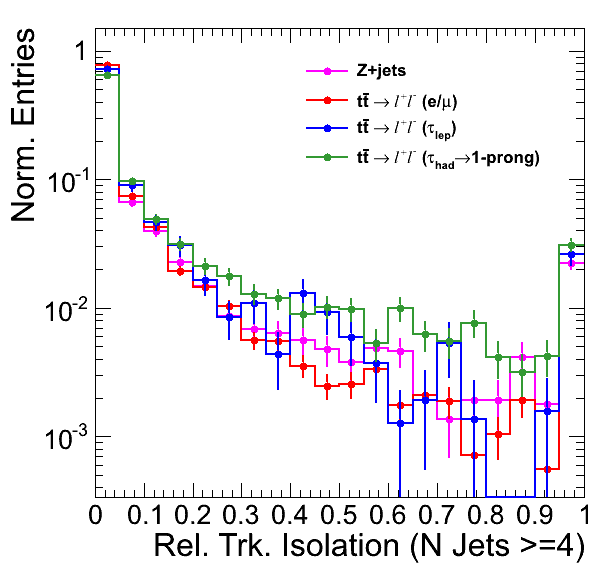
\includegraphics[width=0.5\linewidth]{plots/pfiso_njets4_log.png}%
%	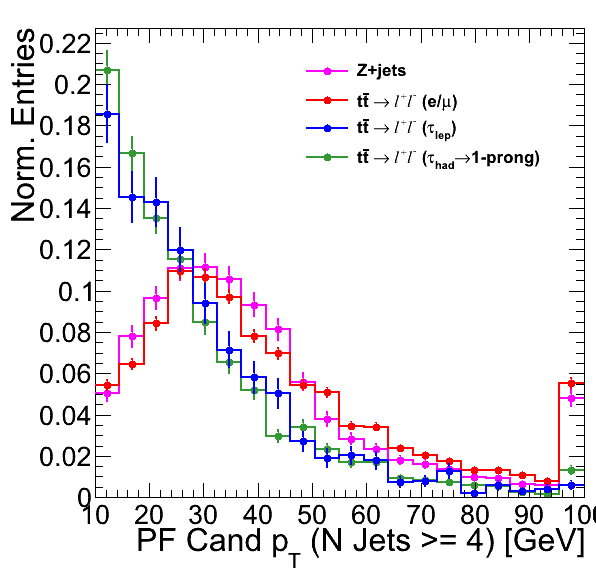
\includegraphics[width=0.5\linewidth]{plots/pfpt_njets4.png}
%	\caption{
%	  \label{fig:reliso}%\protect 
%          Comparison of relative track isolation variable for PF cand probe in Z+jets and ttbar 
%          Z+Jets and ttbar dilepton have similar isolation distributions
%          ttbar with leptonic and single prong taus tend to be less
%          isolated. The difference in the isolation can be attributed
%          to the different \pt\ distribution of the samples, since
%          $\tau$ decay products tend to be softer than leptons arising
%          from \W\ or \Z\ decays.}  
%      \end{center}
%\end{figure}

%	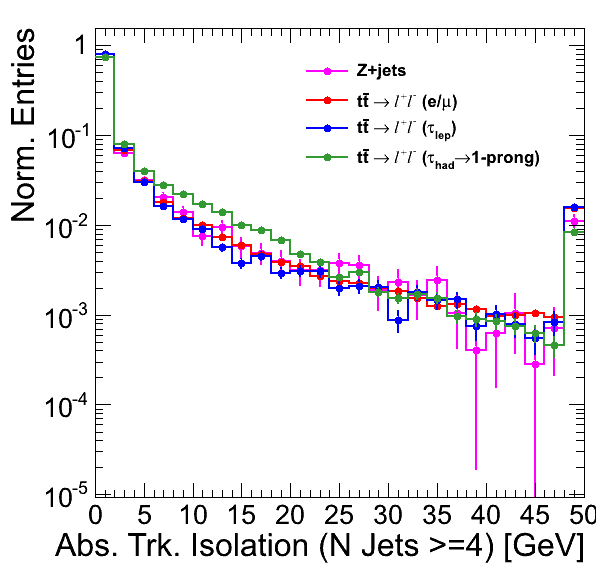
\includegraphics[width=0.5\linewidth]{plots/pfabsiso_njets4_log.png}


%BEGIN SECTION TO WRITE OUT 
%In detail, the procedure to correct the dilepton background is:

%\begin{itemize}
%\item Using tag-and-probe studies, we plot the distribution of {\bf absolute} track isolation for identified probe electrons
%and muons {\bf TODO: need to compare the e vs. $\mu$ track iso distributions, they might differ due to e$\to$e$\gamma$}.
%\item We verify that the distribution of absolute track isolation does not depend on the \pt\ of the probe lepton.
%This is due to the fact that this isolation is from ambient PU and jet activity in the event, which is uncorrelated with
%the lepton \pt {\bf TODO: verify this in data and MC.}.
%\item Our requirement is {\bf relative} track isolation $<$ 0.1. For a given \ttll\ MC event, we determine the \pt of the 2nd
%lepton and translate this to find the corresponding requirement on the {\bf absolute} track isolation, which is simply $0.1\times$\pt.
%\item We measure the efficiency to satisfy this requirement in data and MC, and define a scale-factor $SF_{\epsilon(trk)}$ which
%is the ratio of the data-to-MC efficiencies. This scale-factor is applied to the \ttll\ MC event.
%\item {\bf THING 2 we are unsure about: we can measure this SF for electrons and for muons, but we can't measure it for hadronic 
%tracks from $\tau$ decays. Verena has showed that the absolute track isolation distribution in hadronic $\tau$ tracks is harder due 
%to $\pi^0\to\gamma\gamma$ with $\gamma\to e^+e^-$.}
%\end{itemize} 
%END SECTION TO WRITE OUT 


%{\bf fix me: What you have written in the next paragraph does not
%explain how $\epsilon_{fake}$ is measured.
%Why not measure $\epsilon_{fake}$ in the b-veto region?}

%A measurement of the $\epsilon_{fake}$ in data is non-trivial. However, it is
%possible to correct for differences in the $\epsilon_{fake}$ between data and MC by
%applying an additional scale factor for the single lepton background
%alone, using the sample in the \mt\ peak region. This scale factor is determined after applying the isolated track
%veto and after subtracting the \ttll\ component, corrected for the
%isolation efficiency derived previously. 
%As shown in Figure~\ref{fig:vetoeffcomp}, the efficiency for selecting an
%isolated track in single lepton events is independent of \mt\, so the use of
%an overall scale factor is justified to estimate the contribution in
%the \mt\ tail. 
%
%\begin{figure}[hbt]
%  \begin{center}
%	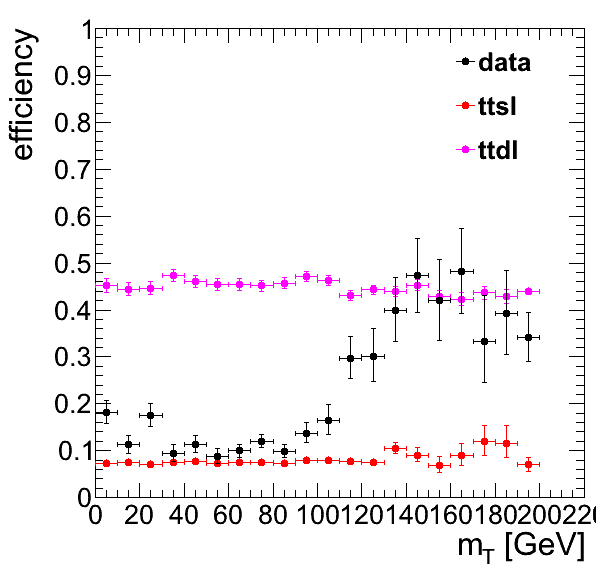
\includegraphics[width=0.5\linewidth]{plots/vetoeff_comp.png}
%	\caption{
%	  \label{fig:vetoeffcomp}%\protect 
%          Efficiency for selecting an isolated track comparing
%          single lepton \ttlj\ and dilepton \ttll\ events in MC and 
%          data as a function of \mt. The
%          efficiencies in \ttlj\ and \ttll\ exhibit no dependence on
%          \mt\, while the data ranges between the two. This behavior
%          is expected since the low \mt\ region is predominantly \ttlj, while the
%          high \mt\ region contains mostly \ttll\ events.}  
%      \end{center}
%\end{figure}



% THIS NEEDS TO BE WRITTEN
